% ----------------------------------------------------------------
% AMS-LaTeX Paper ************************************************
% **** -----------------------------------------------------------
\documentclass[12pt, reqno]{article}
\usepackage{caption}
\usepackage{graphicx}
\usepackage{amsbsy}
\usepackage{bm}
\usepackage{fixmath}
\usepackage{mathrsfs}
\usepackage{caption}
\captionsetup[table]{position=bottom, justification=centering}
\captionsetup[figure]{position=bottom, justification=centering}
\usepackage{epsfig}
\usepackage{eepic}
\usepackage{epic}
\usepackage{float}
\usepackage{amsthm}     %For theorems
\usepackage{bm}
\usepackage{amsmath}
\usepackage{amssymb}
\usepackage{appendix}
\usepackage{setspace} %interlineado
\usepackage{array}
\usepackage{booktabs}
\usepackage{geometry} %Appendix
\usepackage{lipsum}   %Appendix
\usepackage{multirow}
\usepackage{tocbibind}
\usepackage{amsfonts}
\usepackage{paralist}
\usepackage{caption}
\usepackage{subcaption}
\usepackage{geometry}
\usepackage{csquotes}
\usepackage{accents}
\usepackage[multiple, flushmargin]{footmisc}
\usepackage{bigdelim}
\usepackage[hidelinks]{hyperref}
\hypersetup{
    colorlinks=true,
    linkcolor=blue,
    filecolor=magenta,      
    urlcolor=cyan,
}
\usepackage{color}
\usepackage{bbm}
\usepackage{booktabs}
\usepackage{mathptmx}

\usepackage{booktabs}
\usepackage{pdflscape}     % para girar la página (landscape)
\usepackage{caption}
\usepackage{threeparttable} % para notas alineadas al ancho de la tabla

\usepackage[utf8]{inputenc}
\usepackage{booktabs, threeparttable}


% ----------------------------------------------------------------
\vfuzz2pt % Don't report over-full v-boxes if over-edge is small
\hfuzz2pt % Don't report over-full h-boxes if over-edge is small
% THEOREMS -------------------------------------------------------
\newtheorem{thm}{Theorem}
\newtheorem{cor}[thm]{Corollary}
\newtheorem{rem}[thm]{Assumption}
\newtheorem{lem}[thm]{Lemma}
\newtheorem{prop}[thm]{Proposition}
\newtheorem{con}{Assumption}
\geometry{left=1.1811in,right=1.1811in,top=1.1811in,bottom=1.1811in}
%\addtolength{\textwidth}{1.8cm} \addtolength{\voffset}{-0.7cm}
%\addtolength{\textheight}{2.3cm} \addtolength{\hoffset}{-0.7cm}
%\linespread{1.2}
% MATH -----------------------------------------------------------
\setcounter{tocdepth}{2}
\newcommand{\norm}[1]{\left\Vert#1\right\Vert}
\newcommand{\abs}[1]{\left\vert#1\right\vert}
\newcommand{\set}[1]{\left\{#1\right\}}
\newcommand{\Real}{\mathbb R}
\newcommand{\eps}{\varepsilon}
\newcommand{\To}{\longrightarrow}
\newcommand{\BX}{\mathbf{B}(X)}
\newcommand{\A}{\mathcal{A}}
\renewcommand\topfraction{1}
\renewcommand\bottomfraction{1}
\renewcommand\textfraction{0}
\newenvironment{proof}[1][Proof]{\textbf{#1.} }{\ \rule{0.5em}{0.5em}}

% ----------------------------------------------------------------
% ----------------------------------------------------------------

\begin{document}
\title{\vspace{-3.5cm}Disentangling Monetary Policy, Central Bank Information, and Response-to-News Shocks: Evidence from an Emerging Market\footnote{We thank Marco Bassetto, Laurence Ball, Francesco Bianchi, Christopher Carroll, Stelios Fourakis, Raul Ibarra, David Rappoport, Jonathan Wright, as well as participants at the Macro/Finance Seminar at Johns Hopkins University, for helpful comments and suggestions. The views expressed in this paper are those of the author and do not necessarily reflect those of Banco de México and Johns Hopkins University.}}

\author{{{Carlos Alba}\footnote{Department of Economics, Johns Hopkins University. E-mail: calbafa1@jh.edu.}}
\\
{\small{Banco de México and Johns Hopkins University}}}
 %



\date{March $2026$} \maketitle
\vspace{-1cm}
\spacing{1}

% ----------------------------------------------------------------
\begin{abstract}
\noindent
This paper studies the transmission of conventional and unconventional monetary policy in Mexico. Using high-frequency identification techniques, we decompose target-rate and forward-guidance (FG) surprises around central bank announcements into monetary policy (MP), central bank information (CBI), and response-to-news (RN) shocks. We show that failing to disentangle CBI and RN components leads to biased estimates of monetary policy effects, giving rise to counterintuitive results such as expansions in output, rising prices, a depreciation of the domestic currency, and increases in inflation expectations following contractionary target-rate shocks. Once these components are isolated, these anomalies largely disappear. In response to contractionary pure target-rate shocks,  output and prices exhibit a hump-shaped decline, the domestic currency appreciates, and inflation expectations remain well anchored. For unconventional policy, unpurged FG shocks appear to have disproportionately large and immediate effects on economic activity. In addition, inflation expectations tend to rise in response to contractionary FG shocks. Once CBI and RN components are removed, however, the effects of these shocks become more moderate and closely resemble those of pure target-rate shocks. We also show that CBI and RN shocks play distinct contamination roles across policy instruments. While both tend to reverse the effects of target-rate shocks, RN shocks disproportionately amplify and accelerate the transmission of FG shocks, whereas CBI shocks play a more limited role.
\newline
\noindent \textbf{JEL Classification:} E43; E44; E52; E58.
\newline
\noindent \textbf{Keywords:} Monetary Policy; High-Frequency Identification; Forward Guidance; Central Bank Information; Response-to-News; Bayesian VAR; Emerging Market Economies.
\end{abstract}
\bigskip
\bigskip
\bigskip
\bigskip







% ----------------------------------------------------------------
\pagebreak

\section{Introduction}
\spacing{1}
\setcounter{page}{1}

High-frequency changes in interest rates around central bank announcements—commonly referred to as monetary policy or interest rate surprises—have become a widely used proxy for monetary policy (MP) shocks. In advanced economies (AEs), a large literature combines these surprises with vector autoregressive (VAR) models or local projections to study the macroeconomic effects of both conventional and unconventional monetary policies. Applying this methodology to emerging market economies (EMEs), however, poses additional challenges, partly reflecting the more limited availability and shorter time span of high-frequency financial data. Although recent studies have extended high-frequency identification (HFI) techniques to some EMEs, much of this literature does not distinguish between conventional and unconventional MP shocks. As a result, evidence on the macroeconomic effects of forward guidance (FG) in these economies remains limited. Moreover, several studies document puzzling responses to contractionary MP shocks, including a depreciation of the domestic currency, rising prices, and increases in inflation expectations. Such findings are difficult to reconcile with standard macroeconomic models and raise questions about the transmission of monetary policy in EMEs.


A potential explanation for these puzzling findings is that interest rate surprises may not exclusively capture MP shocks, that is, exogenous deviations from a systematic policy rule. In particular, they may also reflect \emph{central bank information (CBI) shocks} (\hyperlink{JK (2020)}{Jarociński and Karadi, 2020}), which arise when the central bank reveals new information about the economic outlook in its announcements while simultaneously adjusting the policy stance in response to that information. In addition, interest rate surprises may reflect \emph{response-to-news (RN) shocks} (\hyperlink{Bauer and Swanson (2023a)}{Bauer and Swanson, 2023a, 2023b}), which arise when markets misperceive the central bank’s policy rule and therefore underestimate or overestimate the strength of its response to observable economic developments. As emphasized in the HFI literature, failing to isolate these shocks from interest rate surprises  may lead to biased estimates of the effects of monetary policy on the economy.

This paper studies the transmission of conventional and unconventional monetary policy in an EME using HFI techniques. Focusing on Mexico as a case study, we decompose interest rate surprises around central bank announcements into MP, CBI, and RN shocks.\footnote{Mexico provides a suitable case study given its small open economy status, credible inflation-targeting regime (\hyperlink{De Pooter et al. (2014)}{De Pooter et al., 2014}; \hyperlink{Beauregard et al. (2024)}{Beauregard et al., 2024}), flexible and market-determined exchange rate (\hyperlink{Ilzetzki et al. (2019)}{Ilzetzki et al., 2019}), and relatively deep and liquid financial markets (\hyperlink{Solis (2023b)}{Solís, 2023a, 2023b}). In particular, the depth and liquidity of Mexican financial markets allow the measurement of interest rate surprises across different maturities and over a relatively long sample period—essential conditions for distinguishing between conventional and unconventional MP shocks and for increasing the overall variation in surprises. This increased variation helps address concerns raised by \hyperlink{Ramey (2016)}{Ramey (2016)} and \hyperlink{Bauer and Swanson (2023b)}{Bauer and Swanson (2023b)} that, in short samples, the macroeconomic effects of monetary policy may be imprecisely estimated.} This decomposition is applied to two types of interest rate surprises: \emph{target-rate surprises}, which capture unexpected changes in the current level of the policy rate, and \emph{FG surprises}, which reflect unexpected revisions to the future path of the policy rate. Using a monthly VAR over the period January 2002 to December 2024, we estimate the dynamic effects of these shocks on a set of macroeconomic and financial variables, including output, prices, the exchange rate, stock prices, inflation expectations, and short- and long-term interest rates.

We construct monetary policy surprises using high-frequency changes in interest rate swaps with maturities ranging from 1 to 12 months around policy announcements. These changes are measured as close-to-close movements from the day preceding the announcement to the announcement day, a standard approach in the EME literature. Following the standard approach of \hyperlink{Gürkaynak et al. (2005)}{Gürkaynak et al. (2005)}, we then extract the first two principal components (PCs) of these changes and rotate them so that the second PC has zero loading on the 1-month swap rate. After this rotation, the first factor can be interpreted as reflecting unexpected changes in the current policy rate—closely tracked by the 1-month swap rate—and we therefore label it the \emph{target-rate surprise}. The second factor captures revisions to the expected near-term policy path, that is, movements in longer-maturity swap rates that are orthogonal to changes in the current policy rate, and we refer to it as the \emph{FG surprise}. 

Following \hyperlink{Bauer and Swanson (2023a, 2023b)}{Bauer and Swanson (2023a, 2023b)}, each interest rate surprise—both target-rate and FG—is regressed on a set of public macroeconomic and financial news released prior to the policy announcement and decomposed into fitted and residual components. The fitted component captures the portion of the surprise that is predictable based on information already incorporated into expectations prior to the announcement. As emphasized by \hyperlink{Bauer and Swanson (2023a, 2023b)}{Bauer and Swanson (2023a, 2023b)}, this component may reflect a stronger or weaker than expected response of the central bank to observable economic developments, potentially arising from market misperceptions of the policy-maker's policy rule. The residual component, by contrast, isolates the portion of the surprise that is orthogonal to prior news and thus provides a cleaner proxy for MP shocks.

Building on \hyperlink{Jarociński and Karadi (2025)}{Jarociński and Karadi (2025)}, we then exploit the co-movement between interest rate and stock price surprises around policy announcements to jointly identify MP, CBI, and RN shocks embedded in both target-rate and FG surprises. Specifically, a \emph{pure MP shock} is identified by a negative co-movement between the residual component of the interest rate surprise and the stock price surprise. This pattern is consistent with an unexpected tightening that raises discount rates and lowers expected future cash flows, leading to an immediate decline in equity prices. When identification is based on the decomposition of the target-rate surprise, we generally refer to the resulting disturbance as a \emph{pure target-rate shock}; when it is based on the decomposition of the FG surprise, we generally refer to it as a \emph{pure FG shock}.

An \emph{RN shock}, in turn, is characterized by a negative co-movement between the fitted component of the interest rate surprise and the stock price surprise. This configuration captures episodes in which the central bank responds more aggressively than markets anticipated to publicly available information. Because that information was largely incorporated into expectations prior to the announcement, the only new element revealed within the announcement window is a stronger-than-expected policy response, which depresses equity prices through standard discount-rate and cash-flow channels.

Finally, a \emph{CBI shock} is associated with a positive co-movement between the interest rate surprise and the stock price surprise. This pattern may arise when the central bank reveals favorable new information about economic fundamentals while simultaneously tightening policy. In such cases, equity prices increase in response to improved growth prospects and higher expected future cash flows, despite the policy tightening.

Our main results indicate that CBI and RN components tend to attenuate—and even reverse—the estimated effects of conventional MP shocks. When these components are not disentangled, impulse responses to contractionary target-rate shocks display several of the puzzles documented in the literature, including expansions in output, rising prices, a depreciation of the domestic currency, and increases in inflation expectations. Once CBI and RN components are isolated, however, these anomalies largely disappear. In response to contractionary pure target-rate shocks, output and prices exhibit a hump-shaped decline, the domestic currency appreciates against the U.S.\ dollar, and inflation expectations remain well anchored. In addition, stock prices decline, and both the
one-year rate and the ten-year yield increase on impact, with the long-term yield rising by
a smaller amount. Overall, these responses are broadly consistent with standard monetary
transmission mechanisms and closely aligned with the empirical evidence for AEs.

The responses to CBI and RN shocks identified from target-rate surprises help shed light on these findings and clarify the role of each component in biasing the transmission of conventional MP shocks. In particular, favorable CBI shocks are associated with increases in interest rates, expansions in output, higher prices, rising inflation expectations, and a depreciation of the Mexican peso. These responses appear to be consistent with a scenario in which the central bank reveals favorable information about economic fundamentals while simultaneously tightening policy to contain emerging inflationary pressures. Hawkish RN shocks generate similar dynamics and may therefore capture episodes in which the central bank tightens policy more aggressively than markets had anticipated in response to observable improvements in economic conditions. In both cases, the contractionary effects of tighter monetary policy appear to be offset by the expansionary forces associated with the underlying macroeconomic developments. Thus, failing to disentangle CBI and RN components may lead to biased estimates of monetary policy effects.




The results for unconventional MP shocks differ in several respects. The impulse responses to contractionary FG shocks do not appear to exhibit a clear attenuation bias potentially arising from RN and CBI components, with the possible exception of inflation expectations, which tend to rise in the short run. Compared with pure target-rate shocks, however, unpurged FG shocks are associated with a disproportionately large and more immediate contraction in domestic activity. While these results could point to a more important role for FG in shaping macroeconomic outcomes, they may also reflect the amplification associated with the \emph{FG puzzle} discussed in the theoretical literature (see \hyperlink{Del Negro et al. (2023)}{Del Negro et al., 2023}), whereby revisions in expectations about the future policy path tend to generate macroeconomic effects that are disproportionately large relative to those of conventional MP shocks. At the same time, the relatively rapid response of output contrasts with the conventional view that monetary policy affects real activity with substantial lags.


Once RN and CBI components are isolated, however, the effects of FG shocks become more moderate and closely resemble those of pure target-rate shocks. Notably, the large and almost immediate decline in output largely disappears. In addition, inflation expectations exhibit a more muted response and appear to remain better anchored following the unconventional policy shock. These results are more consistent with the evidence reported by \hyperlink{Solis (2023b)}{Solís (2023b)}, who shows that FG surprises play an equally important role as target-rate surprises in the transmission of monetary policy to financial markets in Mexico. They also broadly align with the international evidence reported by \hyperlink{Andrade and Ferroni (2021)}{Andrade and Ferroni (2021)} and \hyperlink{Swanson (2021, 2024)}{Swanson (2021, 2024)}, who find that FG shocks tend to generate macroeconomic effects comparable to those of conventional policy shocks.

In general, the impulse responses to CBI and RN shocks identified from FG surprises do not differ markedly from those of pure FG shocks, further suggesting that attenuation bias through these channels  is limited in the case of FG. One possible interpretation is that the central bank responds to evolving demand conditions primarily through adjustments in the policy rate rather than through communication about the future policy path. This behavior may reflect the fact that, in EMEs, FG has typically been used as a complementary rather than a primary policy tool. Unlike in AEs—where central banks were constrained by the effective lower bound and relied more heavily on this unconventional tool—FG in EMEs tends to reinforce and complement policy rate decisions, rather than substitute for them. As a result, CBI and RN shocks may play a more prominent role in attenuating the effects of target-rate surprises than those of FG surprises.

One aspect worth highlighting, however, is the response of domestic output to hawkish RN shocks identified from FG surprises. The dynamics closely resemble those following unpurged FG shocks, suggesting that the amplified and rapid effects of such shocks on economic activity partly reflect RN contamination. One plausible interpretation is that, in the context of FG, market participants tend to overestimate the central bank’s reaction function. For instance, when economic activity is weakening, investors may anticipate a strongly accommodative policy path, whereas the central bank—consistent with the behavior discussed above and its primary mandate of price stability—signals a relatively more hawkish stance or provides little additional guidance due to concerns about inflationary pressures. The resulting impulse responses would then reflect both the contractionary effects of an upward revision in the expected path of policy rates and underlying weakness in output that was already underway, thereby generating disproportionately large and front-loaded declines in activity.

This paper contributes to the literature along three main dimensions. First, it complements \hyperlink{Jarociński and Karadi (2025)}{Jarociński and Karadi (2025)}, who jointly analyze the role of CBI and RN shocks in shaping monetary policy transmission in the U.S., by extending their framework to an EME and examining how these shocks affect the transmission of both conventional and unconventional monetary policy. We show that RN shocks play distinct contamination roles across policy instruments: they tend to attenuate—or even reverse—the effects of target-rate surprises, while amplifying and accelerating the transmission of FG surprises. 

Second, this paper provides new evidence on the macroeconomic effects of FG in EMEs, a dimension that has received relatively limited attention in the existing literature. In particular, we complement \hyperlink{Solis (2023b)}{Solís (2023b)}, who shows that target-rate and FG surprises play a similarly important role in the transmission of monetary policy to financial markets in Mexico. We show that, once purified of CBI and RN components, these surprises also have comparable effects on macroeconomic variables such as output, prices, and inflation expectations. 

Third, we propose an alternative and complementary explanation for several puzzles documented in the literature on monetary transmission in EMEs, where HFI-based evidence has reported counterintuitive responses of exchange rates, prices, and inflation expectations to contractionary MP shocks. We show that these puzzles may arise from failing to disentangle CBI and RN components embedded in interest rate surprises.

The remainder of the paper is organized as follows. \hyperlink{Section 2}{Section~2} reviews the related literature. \hyperlink{Section 3}{Section~3} outlines the construction of monetary policy surprises and the identification strategy used to isolate the shocks of interest. \hyperlink{Section 4}{Section~4} presents the VAR and the data used in the estimation. The empirical results are reported in \hyperlink{Section 5}{Section~5}. \hyperlink{Section 6}{Section~6} concludes.

\section{Related Literature}
\hypertarget{Section 2}{}

This paper relates to the growing body of work that uses HFI to study the macroeconomic effects of monetary policy. Building on early contributions such as \hyperlink{Kuttner (2001)}{Kuttner (2001)} and \hyperlink{Gürkaynak et al. (2005)}{Gürkaynak et al. (2005)}, a large literature combines interest rate surprises with VARs  to estimate the effects of conventional and unconventional MP shocks (e.g., \hyperlink{Gertler and Karadi (2015)}{Gertler and Karadi (2015)};  \hyperlink{Andrade and Ferroni (2021)}{Andrade and Ferroni (2021)}; \hyperlink{Miranda-Agrippino and Ricco (2021)}{Miranda-Agrippino and Ricco (2021)}; \hyperlink{Bauer and Swanson (2023a, 2023b)}{Bauer and Swanson (2023a, 2023b)}; \hyperlink{Swanson (2021, 2024)}{Swanson (2021, 2024)}; \hyperlink{Jarociński and Karadi (2020, 2025)}{Jarociński and Karadi (2020, 2025)}).

In particular, a growing body of research aims to quantify the role of CBI and RN shocks in contaminating interest rate surprises. \hyperlink{Jarociński and Karadi (2020)}{Jarociński and Karadi (2020)} exploit the high-frequency co-movement between interest rate and stock price surprises around FOMC announcements to distinguish between MP and CBI shocks. Their results show that interest rate surprises purged of CBI effects generate a more pronounced contraction in activity and prices than their unpurged counterparts. \hyperlink{Bauer and Swanson (2023a, 2023b)}{Bauer and Swanson (2023a, 2023b)} propose purging interest rate surprises of the component predicted by public news, which reflects RN shocks. MP shocks identified in this way generate stronger contractionary effects. Building on these two strands of the literature, \hyperlink{Jarociński and Karadi (2025)}{Jarociński and Karadi (2025)} propose a unified framework that jointly identifies MP, CBI, and RN shocks. Applying this approach to the U.S., they find robust evidence of CBI shocks but limited evidence that RN shocks play an important role in contaminating interest rate surprises. 

Our paper complements this research by applying the \hyperlink{Jarociński and Karadi (2025)}{Jarociński and Karadi (2025)} framework to an EME and by jointly analyzing the macroeconomic effects of MP, CBI, and RN shocks embedded in both target-rate and FG surprises. We show that both CBI and RN components play an important role in contaminating the transmission of target-rate surprises by attenuating and even reversing their estimated effects. Notably, for FG surprises, RN components appear to distort the estimated transmission by disproportionately amplifying and accelerating their effects, particularly on output, while CBI components mainly generate a small attenuation bias in the response of inflation expectations.



We also contribute to the literature that analyzes the macroeconomic effects of FG. For AEs, \hyperlink{Campbell et al. (2012)}{Campbell et al. (2012)} and \hyperlink{Andrade and Ferroni (2021)}{Andrade and Ferroni (2021)} emphasize that FG surprises may combine “Odyssean” policy commitments with “Delphic” signals about future macroeconomic conditions. \hyperlink{Andrade and Ferroni (2021)}{Andrade and Ferroni (2021)} show that these “Delphic” signals can reverse the estimated effects of FG shocks on prices, expectations, and credit spreads. By contrast, for real activity, these signals do not appear to generate a clear attenuation bias. \hyperlink{Swanson (2024)}{Swanson (2024)} shows that FG surprises in the U.S. may be contaminated by RN components, which tend to attenuate their estimated macroeconomic effects. For the particular case of Mexico, \hyperlink{Solis (2023b)}{Solís (2023b)} shows that interest rate surprises contain two distinct dimensions—target-rate and FG surprises—that play a similarly important role in the transmission of monetary policy to financial markets. 

We complement \hyperlink{Solis (2023b)}{Solís (2023b)} by disentangling target-rate and FG surprises into MP, CBI, and RN components and by examining their macroeconomic effects on variables such as output, prices, and inflation expectations. In doing so, we also complement the evidence in \hyperlink{Swanson (2024)}{Swanson (2024)} by showing that, in the context of an EME, RN components may disproportionately amplify and accelerate the effects of FG shocks. In line with \hyperlink{Andrade and Ferroni (2021)}{Andrade and Ferroni (2021)}, we find that CBI shocks tend to attenuate the estimated effects of FG shocks on inflation expectations, but do not play a significant role in biasing their transmission to real activity.

Finally, this paper contributes to the literature on monetary transmission in EMEs, where empirical work using HFI has documented puzzling responses of exchange rates, prices, and inflation expectations to contractionary MP shocks. \hyperlink{Aruoba et al. (2021)}{Aruoba et al. (2021)} show that the domestic currency depreciates and inflation expectations rise following an unexpected tightening in Chile. Using a panel of EMEs, \hyperlink{Bolhuis et al. (2024)}{Bolhuis et al. (2024)} document an average depreciation of the exchange rate after contractionary MP shocks. More recently, \hyperlink{Witheridge (2024)}{Witheridge (2024)} reports increases in prices and inflation expectations following an unexpected tightening and interprets them as evidence of fiscal-led policy dynamics in some EMEs, including Mexico. \hyperlink{Solís (2023a)}{Solís (2023a)} also finds evidence of an exchange rate puzzle in Mexico but shows that it largely disappears when the exchange rate response around monetary policy announcements is measured using intraday data.

We contribute to this literature by proposing an alternative and complementary explanation for the emergence of these puzzles: the failure to account for informational components embedded in interest rate surprises. We show that once CBI and RN components are isolated, impulse responses to an MP shock become broadly consistent with standard transmission mechanisms. Importantly, we conduct the analysis using daily data, which is particularly valuable in EMEs where access to intraday financial data may be limited.





\section{High-Frequency Identification of MP, RN, and CBI Shocks}
\hypertarget{Section 3}{}

This section outlines the construction of target-rate and FG surprises, as well as the identification strategy used to isolate MP, RN, and CBI shocks embedded in these measures. Our approach closely follows the framework of \hyperlink{Jarociński and Karadi (2025)}{Jarociński and Karadi (2025)} and proceeds in three stages. First, we construct target-rate and FG surprises using high-frequency changes in interest rate swaps around monetary policy announcements in Mexico. Second, in the spirit of \hyperlink{Bauer and Swanson (2023a, 2023b)}{Bauer and Swanson (2023a, 2023b)}, we decompose these surprises into predictable and residual components by regressing each interest rate surprise on a set of macroeconomic and financial news observable prior to the policy announcement. Finally, we exploit the high-frequency co-movement between interest rate and stock price surprises to jointly identify the shocks of interest.



\subsection{Constructing Target-Rate and FG Surprises}

Following \hyperlink{Andrade and Ferroni (2021)}{Andrade and Ferroni (2021)}, \hyperlink{Solis (2023a)}{Solís (2023a, 2023b)}, and \hyperlink{Bolhuis et al. (2024)}{Bolhuis et al. (2024)}, we construct monetary policy surprises using high-frequency changes in interest rate swaps with maturities of 1, 3, 6, 9, and 12 months around monetary policy announcements. These surprises reflect revisions in expectations regarding both the current level of the policy rate and its future path.\footnote{The Mexican swap market references the 28-day interbank rate (TIIE-28), which is closely tied to the policy rate and serves as a benchmark for short-term bank lending.} Given the lack of intraday data, high-frequency changes in swap rates are measured as close-to-close movements from the trading day preceding the announcement to the day of the announcement. This approach is standard in the literature on EMEs, where intraday financial data are typically unavailable (see \hyperlink{Bolhuis et al. (2024)}{Bolhuis et al. (2024)}, \hyperlink{Witheridge (2024)}{Witheridge (2024)}, \hyperlink{Gomes et al. (2023)}{Gomes et al. (2023)}, and \hyperlink{Aruoba et al. (2021)}{Aruoba et al. (2021)}). Our sample includes 214 scheduled monetary policy announcements over the period January~2002 to December~2024. The starting date reflects the availability of bond yield data used in the estimations below and closely coincides with the adoption of an inflation-targeting regime by the central bank of Mexico in 2001.

Following the standard approach of \hyperlink{Gürkaynak et al. (2005)}{Gürkaynak et al. (2005)}, we extract the first two principal components (PCs) of these high-frequency changes in interest rate swaps and rotate them so that the second PC has zero loading on the 1-month swap rate. After this rotation, the first factor can be interpreted as reflecting unexpected changes in the current policy rate—closely tracked by the 1-month swap rate—and we therefore label it the \emph{target-rate surprise}. The second factor captures revisions to the expected near-term policy path, that is, movements in longer-maturity swap rates that are orthogonal to changes in the current policy rate, and we refer to it as the \emph{FG surprise}. For comparability and ease of interpretation, both surprises are rescaled so that the target-rate surprise moves one-for-one with changes in the 1-month swap rate, while the FG surprise affects the 12-month swap rate by the same magnitude as the target-rate surprise.

\subsection{Decomposing Target-Rate and FG Surprises}

In this section, we decompose the target-rate and FG surprises into two components: one that is predictable ex post using publicly available information prior to the announcement, and a residual component orthogonal to this information set. This decomposition follows the logic of \hyperlink{Bauer and Swanson (2023a, 2023b)}{Bauer and Swanson (2023a, 2023b)}, who highlight that interest rate surprises may capture not only exogenous MP shocks but also unexpected responses of the central bank to the state of the economy, particularly when market expectations about the policy reaction function are imperfect.

Formally, for each policy announcement $t$, we estimate
\begin{equation}
mps_t = \alpha + X_{t-}'\beta + u_t,
\end{equation}
where $mps_t$ denotes either the target-rate or the FG surprise, $X_{t-}$ collects macroeconomic and financial variables observable before the policy announcement (as indicated by the time subscript $t-$), and $u_t$ is the residual. We define the fitted component as $\text{FIT}_t \equiv \widehat{\alpha} + X_{t-}'\widehat{\beta}$ and the residual component as $\text{RES}_t \equiv \widehat{u}_t$, where by construction $\text{RES}_t$ is orthogonal to all variables included in $X_{t-}$. The fitted component captures the portion of the surprise that is explained by the pre-announcement information set and may be interpreted as reflecting revisions in expectations about the systematic policy response to news—that is, the RN component. The residual component isolates the unpredictable part of the surprise, which is more closely related to exogenous deviations from the systematic policy rule.

Empirical studies, including  \hyperlink{Cieslak (2018)}{Cieslak (2018)}, \hyperlink{Bauer and Swanson (2023a, 2023b)}{Bauer and Swanson (2023a, 2023b)}, and \hyperlink{Swanson (2024)}{Swanson (2024)}, among others, document a range of macroeconomic and financial variables that help predict interest rate surprises ex post. We incorporate several of these variables into $X_{t-}$, while also including a small set of additional variables that may be particularly relevant for an EME such as Mexico. Given Mexico’s status as a small open economy with strong economic linkages to the United States, $X_{t-}$ includes both domestic and external variables, primarily capturing U.S. financial and macroeconomic conditions, along with global commodity price movements.\footnote{Mexico is a small open economy with strong real and financial linkages to the U.S., often viewed as the “center country” in studies of small open economies. Roughly 80\% of Mexican exports are directed to the U.S., and a large share of foreign direct investment originates there. Prior work documents close trade and financial integration between the two economies, including substantial co-movement in term premia and short-term interest rates [see, for instance, \hyperlink{Fink (2015)}{Fink and Schüler (2015)} and \hyperlink{Carrillo et al. (2020)}{Carrillo et al. (2020)}].}


To capture domestic financial conditions, we include the log change in the nominal peso--U.S.\ dollar exchange rate and changes in the volatility implied by one-month options on the Mexican peso, both measured from three months prior to the announcement to the day before the announcement.\footnote{The volatility implied by one-month options on the Mexican peso reflects market expectations about near-term exchange rate uncertainty. This measure is widely followed by market participants and is regularly discussed in the Central Bank of Mexico’s quarterly inflation reports.} In addition, we consider three-month changes in the interbank funding rate and in the two-year Mexican government bond yield.\footnote{The interbank funding rate captures short-term conditions in the domestic money market and is closely tied to the monetary policy rate.}  To capture domestic macroeconomic conditions, we include log changes in the Overall Indicator of Economic Activity (IGAE, by its Spanish acronym) and in the core Consumer Price Index (CPI), measured from six months prior to the most recent data release available before the policy announcement.\footnotemark
\footnotetext{The IGAE follows the methodology and conceptual framework of the national accounts. The correlation between IGAE and GDP, both measured in quarterly percentage changes, is 0.99. The IGAE is subject to revisions, so the data available at a given point in time may differ from the final revised values released by the statistical office. Although the use of real-time data would be desirable, such data are unavailable for Mexican output. We therefore rely on revised data in our estimations.}\textsuperscript{,}\footnotemark
\footnotetext{ IGAE is released with a delay of approximately seven to eight weeks (approximated by 42 trading days), while consumer prices are typically released with a lag of about two weeks (approximated by 10 trading days).}

As external financial variables, we include log changes in the Standard \& Poor’s 500 stock index, changes in two-year and ten-year U.S.\ Treasury yields, and the log change in Brent crude oil prices, all measured over a three-month horizon prior to the policy announcement. For external macroeconomic conditions, we consider log changes in U.S.\ industrial production and in the U.S.\ Consumer Price Index, measured from six months prior to the most recent data release available before the policy announcement. Finally, following \hyperlink{Miranda-Agrippino and Ricco (2021)}{Miranda-Agrippino and Ricco (2021)} and \hyperlink{Swanson (2024)}{Swanson (2024)}, we include one lag of the dependent variable to account for potential serial correlation in monetary policy surprises.


\hyperlink{Table 1}{Table~1} reports the results from projecting target-rate and FG surprises onto the set of macroeconomic and financial variables described above, using the full sample from January 2002 to December 2024.\footnote{Monetary policy surprises, changes in interest rates, and variations in implied exchange rate volatility are expressed in basis points. Changes in real activity, consumer prices, oil prices, asset prices, and the exchange rate are measured as log differences multiplied by 100. Three-month windows correspond to 65 trading days. U.S.\ consumer prices and U.S.\ industrial production are typically released with a lag of about two weeks.} Results for target-rate surprises are reported in the first column, while those for FG surprises are shown in the second column. Standard errors (in parentheses) are computed using heteroskedasticity- and autocorrelation-consistent (HAC) estimators. As can be seen, the set of regressors explains a non-negligible share of the variation in monetary policy surprises, with $R^2$ values of approximately 22\% for target-rate surprises and 15\% for FG surprises, broadly in line with estimates reported in the related literature.\footnotemark
\footnotetext{The null hypothesis of no predictability is rejected at the 1\% significance level for target-rate surprises and at the 10\% level for FG surprises, based on heteroskedasticity- and autocorrelation-robust Wald tests.}\textsuperscript{,}\footnotemark
\footnotetext{As robustness exercises, we conduct two additional checks. First, we estimate an extended specification that augments the baseline regression with a broader set of controls commonly used in the literature. The resulting impulse responses based on the fitted and residual components remain largely unchanged (see \hyperlink{Table B.1}{Table~B.1} and \hyperlink{Figure B.1}{Figures~B.1 and B.2} in \hyperlink{Appendix B}{Appendix~B}). Second, we implement LASSO-based projections to allow the data to select the most relevant predictors (see \hyperlink{Table B.2}{Table~B.2} and \hyperlink{Figure B.3}{Figures~B.3 and B.4} in \hyperlink{Appendix B}{Appendix~B}). For target-rate surprises, the selected variables broadly coincide with those in the baseline information set, whereas for FG surprises the procedure selects a substantially smaller subset. The corresponding impulse responses remain broadly consistent with the baseline results, although the separation between MP and RN shocks becomes less pronounced, particularly for target-rate surprises, resulting in attenuated impulse responses to MP shocks. Overall, we interpret these results as suggesting that the baseline specification is sufficiently rich to capture an important share of the systematic component of monetary policy surprises that could otherwise introduce bias into our structural estimates if not properly separated.}


\begin{table}[t]
\begin{center}
\resizebox{0.58\textwidth}{!}{
\begin{tabular}{lcc}
\toprule
 & Target-rate surprise & FG surprise \\
\midrule
\multicolumn{3}{l}{\textbf{\emph{Domestic news}}} \\[0.2em]
$\Delta \log$ domestic output (6m)                     
& $-$0.036  
& 0.239  \\
& (0.177) 
& (0.674) \\

$\Delta \log$ CPI (6m)                      
& $-$0.287  
& 2.109 \\
& (1.246) 
& (3.483) \\

$\Delta \log$ MXN/USD (3m)            
& 0.007  
& 0.962** \\
& (0.168) 
& (0.410) \\

$\Delta$ FX implied volatility (3m)   
& 0.004*  
& $-$0.010** \\
& (0.002) 
& (0.004) \\

$\Delta$ Interbank rate (3m)          
& 0.022  
& $-$0.010 \\
& (0.015) 
& (0.027) \\

$\Delta$ 2-year gov. yield (3m)       
& 0.030*  
& 0.008  \\
& (0.015) 
& (0.039) \\[0.4em]

\multicolumn{3}{l}{\textbf{\emph{External news}}} \\[0.2em]
$\Delta \log$ Industrial prod. (6m)        
& 0.007  
& 0.782  \\
& (0.261) 
& (0.849) \\

$\Delta \log$ US CPI (6m)                     
& 1.201  
& $-$1.219 \\
& (0.979) 
& (2.053) \\

$\Delta \log$ S\&P 500 (3m)            
& 0.129  
& 0.252  \\
& (0.143) 
& (0.337) \\

$\Delta$ 2-year Treasury yield (3m)   
& $-$0.007  
& 0.091**  \\
& (0.021) 
& (0.040) \\

$\Delta$ 10-year Treasury yield (3m)  
& $-$0.052* 
& $-$0.095*  \\
& (0.026) 
& (0.054) \\

$\Delta \log$ Brent oil price (3m)       
& 0.078* 
& 0.123  \\
& (0.045) 
& (0.110) \\[0.4em]

\multicolumn{3}{l}{\textbf{\emph{Lagged monetary policy surprises}}} \\[0.2em]
Surprise$_{t-1}$                      
& 0.021  
& $-$0.225** \\
& (0.120)  
& (0.097) \\[0.4em]

\midrule
$R^2$              & 0.224 & 0.154 \\
Adjusted $R^2$     & 0.173 & 0.099 \\
Observations       & 213   & 213   \\
\bottomrule
\end{tabular}}
\caption{Regressions of High-Frequency Monetary Policy Surprises on Macroeconomic and Financial News}
\end{center}
\begin{footnotesize}
\textit{Notes}: This table reports coefficient estimates from regressions of target-rate and forward guidance (FG) surprises on macroeconomic and financial news released prior to the monetary policy announcement. Standard errors (in parentheses) are heteroskedasticity- and autocorrelation-consistent (HAC), computed using a Newey--West estimator. $^{*}$, $^{**}$, and $^{***}$ denote significance at the 10\%, 5\%, and 1\% levels, respectively. \\
\textit{Sources}: Banco de México, INEGI, FRED, and Bloomberg.
\end{footnotesize}
\end{table}

These results indicate that interest rate surprises are correlated with publicly available economic information prior to policy announcements. While the underlying mechanisms are beyond the scope of this exercise, this pattern is consistent with the possibility that market expectations about the policy reaction function are imperfect. For the VAR analysis, however, the precise interpretation of this correlation is of secondary importance, as emphasized by \hyperlink{Swanson (2024)}{Swanson (2024)}. What matters is the empirical regularity that interest rate surprises are not fully orthogonal to pre-announcement economic and financial conditions. As we show below, failing to account for this feature leads to impulse response functions that display puzzling or potentially misleading dynamics following an MP shock.

\subsection{Disentangling MP, RN, and CBI Shocks embedded in Target-Rate and FG Surprises}

Building on \hyperlink{Jarociński and Karadi (2025)}{Jarociński and Karadi (2025)}, we exploit the high-frequency co-movement between interest rate and stock price surprises to identify MP, RN, and CBI shocks using sign and magnitude restrictions. The identification is implemented separately for target-rate and FG surprises. In each case, we use the corresponding fitted and residual components—denoted by $(\text{FIT}^{TR}, \text{RES}^{TR})$ for target-rate surprises and $(\text{FIT}^{FG}, \text{RES}^{FG})$ for FG surprises—together with a common stock-price surprise measure, $\text{SP}$. The latter is constructed as the log difference of the Mexican Stock Market Index (IPC) between the trading day preceding the policy announcement and the day of the announcement.


Our identification strategy assumes that, within a daily window around policy announcements, interest rate and equity-price surprises are predominantly driven by three structural disturbances—MP, RN, and CBI shocks. This assumption is stronger than in studies for AEs that rely on intraday windows surrounding policy announcements. Nevertheless, intraday financial data are typically unavailable for EMEs, and much of the literature therefore relies on daily windows for this type of analysis.\footnote{One exception is \hyperlink{Solis (2023a)}{Solís (2023a, 2023b)}, who employs intraday data on interest rate swaps for Mexico. However, the available dataset begins only in 2011 and lacks intraday observations for several of the interest rate swaps considered in our analysis, as well as for equity prices, which are central to our identification strategy. As emphasized by \hyperlink{Solis (2023a)}{Solís (2023a, 2023b)}, measurement error in daily swap-rate changes around policy announcements appears to be limited, as the correlation between intraday and daily changes in swap rates is close to one. To alleviate concerns that the equity-price surprise may partly reflect global financial developments unrelated to domestic monetary policy news, we orthogonalize our equity-price surprise with respect to contemporaneous changes in the S\&P~500 index, the VIX index, and the two-year Treasury yield as a robustness check. The results of this regression are reported in \hyperlink{Table B.3}{Table~B.3} in \hyperlink{Appendix B}{Appendix~B}. The corresponding impulse responses obtained using the orthogonalized measure are very similar to those reported in the baseline specification (see \hyperlink{Figure B.5}{Figures~B.5 and B.6} in \hyperlink{Appendix B}{Appendix~B}).
} In addition, we assume that each disturbance generates a distinct pattern of co-movement between interest rate and equity-price surprises.





A \emph{\textbf{pure MP shock}} is characterized by a negative co-movement between the residual component of the interest rate surprise—either $\text{RES}^{TR}$ or $\text{RES}^{FG}$—and the stock price surprise. This pattern is consistent with an unexpected policy tightening that raises discount rates and lowers expected future cash flows, leading to an immediate decline in equity prices. When identification is based on the decomposition of the target-rate surprise, we generally refer to the resulting disturbance as a \emph{pure target-rate shock}; when it is based on the decomposition of the FG surprise, we generally refer to it as a \emph{pure FG shock}.

An \emph{\textbf{RN shock}} is identified by a negative co-movement between the fitted component of the interest rate surprise—either $\text{FIT}^{TR}$ or $\text{FIT}^{FG}$—and the stock price surprise. This shock captures episodes in which the central bank responds more aggressively than markets anticipated to publicly available information that was already incorporated into expectations prior to the announcement. As a result, the main information revealed within the announcement window is the stronger-than-expected monetary policy response, which depresses equity prices through standard discount-rate and cash-flow channels.

A \emph{\textbf{CBI shock}} is identified by a positive co-movement between the overall monetary policy surprise—defined as $\text{FIT}^{j}+\text{RES}^{j}$—and the equity-price surprise. This pattern may arise when the central bank reveals favorable new information about economic fundamentals while simultaneously tightening policy. In such cases, equity prices increase in response to improved growth prospects and higher expected future cash flows, despite the policy tightening.

These assumptions are summarized by the following impact representation:
\begin{equation}
\begin{pmatrix}
\text{RES}^{j} \\
\text{FIT}^{j} \\
\text{SP}
\end{pmatrix}
=
\begin{pmatrix}
+ & c_{12} & c_{13} \\
c_{21} & + & c_{23} \\
- & - & +
\end{pmatrix}
\begin{pmatrix}
\text{MP}^{j} \\
\text{RN}^{j} \\
\text{CBI}^{j}
\end{pmatrix},
\quad j \in \{\text{TR}, \text{FG}\},
\end{equation}
together with the restriction that the overall policy surprise (the sum of fitted and residual components) rises on impact after a favorable CBI shock:
\begin{equation}
\label{eq:cbi_policy_surprise}
(c_{13}+c_{23}) > 0.
\end{equation}

Finally, we impose magnitude restrictions to ensure that the FIT--RES decomposition provides informative proxies for the MP and RN shocks:
\begin{equation}
\label{eq:mag_res_mp}
|c_{12}| < c_{11},
\end{equation}
\begin{equation}
\label{eq:mag_res_rn}
|c_{21}| < c_{22}.
\end{equation}
Restriction \eqref{eq:mag_res_mp} ensures that the residual component loads more strongly on the MP shock than on the RN shock, while restriction \eqref{eq:mag_res_rn} ensures that the fitted component loads more strongly on the RN shock than on the MP shock. 



\section{VAR Model for a Small Open Economy}
\hypertarget{Section 4}{}

To analyze the macroeconomic effects of MP, RN, and CBI shocks, we estimate a monthly Bayesian VAR model. The reduced-form representation of the VAR is given by
\begin{equation}
  \boldsymbol{Y}_t
  = \boldsymbol{c}
  + \sum_{p=1}^{P} \boldsymbol{B}^{p}\,\boldsymbol{Y}_{t-p}
  + \boldsymbol{\delta}\,\boldsymbol{Z}_t
  + \boldsymbol{u}_t ,
\end{equation}
where the vector $\boldsymbol{Y}_t$ stacks high-frequency surprises and low-frequency macroeconomic and financial variables observed in month $t$, $\boldsymbol{c}$ collects intercepts, $\boldsymbol{B}^{p}$ denotes the lag-$p$ coefficient matrices, $\boldsymbol{Z}_t$ collects exogenous controls, and $\boldsymbol{u}_t \sim \mathcal{N}\!\left(\mathbf{0},\boldsymbol{\Sigma}\right)$. In particular, we partition $\boldsymbol{Y}_t$ as

\[
\boldsymbol{Y}_t =
\begin{pmatrix}
\boldsymbol{m}_t^{\,j} \\
\boldsymbol{y}_t
\end{pmatrix},
\qquad j \in \{\text{TR}, \text{FG}\},
\]
where $\boldsymbol{m}_t^{\,j}$ collects the fitted and residual components $(\text{FIT}_t^{\,j}, \text{RES}_t^{\,j})$ associated with either the target-rate or the FG surprise, together with the equity-price surprise $\text{SP}_t$. In turn, $\boldsymbol{y}_t$ denotes a vector of domestic macroeconomic and financial variables described below.\footnote{Note that we do not treat high-frequency surprises as a separate block that is exogenous with respect to the rest of the variables. Instead, these surprises are allowed to interact with the rest of the system, consistent with our departure from the assumption that they are fully exogenous and unpredictable. For robustness, we also estimate a specification in which high-frequency surprises are included as an exogenous block. The results remain consistent and are reported in \hyperlink{Figure B.7}{Figures~B.7 and B.8} of \hyperlink{Appendix B}{Appendix~B}.} As in \hyperlink{JK (2020)}{Jarociński and Karadi (2020, 2025)} and \hyperlink{Breitenlechner (2021)}{Breitenlechner et al. (2021)}, the high-frequency surprises are aggregated to the monthly frequency by summing surprises within month $t$, assigning a value of zero to months with no policy announcements. Following previous studies for small open economies, we include foreign exogenous controls $\boldsymbol{Z}_t$—primarily U.S.\ variables—which are allowed to affect domestic variables contemporaneously, but not vice versa.\footnote{See, for instance, \hyperlink{Bjørnland (2009)}{Bjørnland (2009)}, \hyperlink{Ibarra (2016)}{Ibarra (2016)}, \hyperlink{Capistrán et al. (2019)}{Capistrán et al. (2019)}, and \hyperlink{Kim and Lim (2022)}{Kim and Lim (2022)}, among others.} In our baseline specification, we include one lag, which is common in studies of monetary policy transmission in EMEs.\footnote{See, e.g., \hyperlink{Canova (2005)}{Canova (2005)}, \hyperlink{Georgiadis (2016)}{Georgiadis (2016)}, and \hyperlink{Dahlhaus et al. (2018)}{Dahlhaus et al. (2018)}.} The set of domestic macroeconomic and financial variables, as well as the exogenous foreign variables included in the VAR model, is presented in \hyperlink{Table 3}{Table~2}.\footnote{All domestic and foreign financial variables are measured at end-of-month values.}




Regarding Mexican macro-financial variables, we include the one-year government bond yield, $i_t^{1y}$, and the ten-year government bond yield, $i_t^{10y}$.\footnote{We use zero-coupon yields at both maturities to ensure comparability, since coupon-bearing bonds differ across maturities. As robustness checks, we conduct two additional exercises. First, we replace the one-year government bond yield with the two-year government bond yield. Second, we make the same replacement and additionally include the interbank funding interest rate. The results remain consistent with our baseline specification and are reported in \hyperlink{Figure B.9}{Figures B.9--B.12} of \hyperlink{Appendix B}{Appendix B}.} The one-year yield reflects both the current policy stance and expectations about near-term policy adjustments \hyperlink{Gertler and Karadi (2015)}{(Gertler and Karadi, 2015)}. The ten-year yield allows us to assess the impact on long-term rates, which are especially relevant for firms’ and households’ decisions \hyperlink{Andrade and Ferroni (2021)}{(Andrade and Ferroni, 2021)}. For real activity, we use an interpolated monthly GDP series, $y_t$, using the approach of \hyperlink{Elizondo (2012)}{Elizondo (2012)}.\footnote{\hyperlink{Elizondo (2012)}{Elizondo (2012)} employs a Kalman filter to interpolate the monthly GDP series using the IGAE index, which is available at a monthly frequency. As a robustness check, we use the IGAE index as an alternative measure of economic activity in Mexico. The results, reported in \hyperlink{Figure B.13}{Figures B.13 and B.14} of \hyperlink{Appendix B}{Appendix B}, are consistent with our baseline specification.} For prices, we use the core Consumer Price Index, $p_t$, which is seasonally adjusted with the X13-ARIMA method.\footnote{As a robustness check, we use the headline CPI instead of the core index. The resulting impulse responses remain consistent with our baseline specification and are reported in \hyperlink{Figure B.15}{Figures B.15 and B.16} of \hyperlink{Appendix B}{Appendix B}.} We also include the nominal peso--U.S.\ dollar exchange rate, $s_t$, the Mexican Stock Market Index, $ipc_t$, and 12-month-ahead inflation expectations, denoted by $\pi^{e}_{t}$.\footnote{12-month-ahead inflation expectations are obtained from the Survey of Professional Forecasters published by Banco de México. \hyperlink{Capistran et al. (2010)}{Capistrán et al. (2010)} find that inflation forecasts from Banco de México’s survey of professional forecasters outperform those from traditional benchmarks, including univariate and multivariate time-series models.}




\begin{table}[t]
\hypertarget{Table 2}{}
\begin{center}
\resizebox{13cm}{!}{
\begin{tabular}{l l l l}
\toprule
Series & Definition & Transformation & Source\\
\midrule
\multicolumn{4}{c}{\textbf{Domestic variables in }$\boldsymbol{y}_t$} \\
\midrule
$i_t^{1y}$ & 1-year government bond yield & No transformation & Banco de México \\
$i_t^{10y}$ & 10-year government bond yield  & No transformation & Banco de México \\
${ipc}_t$ & Mexican Stock Market Index & $\ln({ipc}_t)$ & Grupo BMV \\
$s_t$ & MXN per USD exchange rate & $\ln(s_t)$ & Banco de México \\
$y_t$ & Interpolated GDP & $\ln(y_t)$ & \hyperlink{Elizondo (2012)}{Elizondo (2012)} \\
$p_t$ & Core consumer price index (CPI)  & $\ln(p_t)$ & INEGI \\
$\pi^{e}_{t}$ & 12-month-ahead inflation expectations  & No transformation & Banco de México \\
\midrule
\multicolumn{4}{c}{\textbf{Exogenous variables in }$\boldsymbol{Z}_t$} \\
\midrule
$i_t^{2*}$ & U.S. 2-year Treasury yield & No transformation & FRED \\
${sp500}_t$ & S\&P 500 index & $\ln({sp500}_t)$ & Bloomberg \\
${vix}_t$ & VIX index & $\ln({vix}_t)$ & Bloomberg \\
$y_t^{*}$ & U.S. Industrial Production & $\ln(y_t^{*})$ & FRED \\
 $p_t^{*}$ & U.S. CPI & $\ln(p_t^{*})$ & FRED \\
${oil}_t$ & Brent crude oil price & $\ln({oil}_t)$ & FRED \\
\bottomrule
\end{tabular}}
\caption{Data Description}
\end{center}
\end{table}

In the vector of exogenous controls $\boldsymbol{Z}_t$, we include the U.S.\ two-year Treasury yield, $i_t^{2*}$, as movements in U.S.\ rates spill over to Mexican yields via portfolio rebalancing and term-structure arbitrage, thereby affecting domestic macroeconomic and financial conditions. As discussed by \hyperlink{Swanson and Williams (2014)}{Swanson and Williams (2014)}, \hyperlink{Gertler and Karadi (2015)}{Gertler and Karadi (2015)}, and \hyperlink{Bauer and Swanson (2023a)}{Bauer and Swanson (2023a)}, the two-year Treasury yield was essentially unconstrained during the zero lower bound period (2009--2015), making it an informative measure of the overall stance of U.S.\ monetary policy.\footnote{As a robustness check, we replace the U.S.\ two-year Treasury yield with the U.S.\ shadow interest rate constructed by \hyperlink{Wu and Xia (2016)}{Wu and Xia (2016)}. The resulting impulse responses remain consistent with our baseline specification and are reported in \hyperlink{Figure B.17}{Figures B.17 and B.18} of \hyperlink{Appendix B}{Appendix B}.} We also include the S\&P~500 index to capture shifts in external financial conditions that may propagate to Mexico. U.S.\ industrial production and the consumer price index, $(y_t^*, p_t^*)$, proxy foreign demand and external price pressures, respectively. The VIX index is included as a standard proxy for risk aversion \hyperlink{Gambacorta et al. (2014)}{(Gambacorta et al., 2014)}; \hyperlink{MacDonald and Popiel (2020)}{(MacDonald and Popiel, 2020)}, and the Brent crude oil price, given its relevance for Mexico’s terms of trade \hyperlink{Capistrán et al. (2019)}{(Capistrán et al., 2019)}. Finally, following \hyperlink{Ng (2021)}{Ng (2021)}, \hyperlink{Evgenidis and Fasianos (2023)}{Evgenidis and Fasianos (2023)}, and \hyperlink{Carrillo et al. (2025)}{Carrillo et al. (2025)}, among others, we include monthly dummy variables to account for the unprecedented disruptions associated with the COVID-19 pandemic in our estimates. Specifically, we include separate dummies for each month from April to September 2020, which allow for temporary intercept shifts during the most disrupted period.\footnote{April--September 2020 corresponds to the period of particularly severe economic disruptions in Mexico (\hyperlink{Banco de Mexico (2020)}{Banco de México, 2020a, 2020b}). A related approach commonly used in the literature is to construct outlier dummies by flagging observations that exceed $n$ times the interquartile range from the sample median (\hyperlink{Stock and Watson (2002)}{Stock and Watson, 2002}). Setting $n=2.5$ and examining outliers in measures of economic activity yields a set of pandemic dummies that is essentially unchanged. As additional robustness checks, we perform two exercises. First, we extend the pandemic dummies through December 2020, following \hyperlink{Carrillo et al. (2025)}{Carrillo et al. (2025)}. Second, we re-estimate the model using a sample that ends in 2019, as is common in the related literature. In both cases, the resulting impulse responses remain broadly consistent with our baseline specification and are reported in \hyperlink{Figure B.19}{Figures B.19--B.22} of \hyperlink{Appendix B}{Appendix B}.}



We estimate the model using a Bayesian approach, which is standard in the sign restrictions literature. In particular, we employ the Minnesota prior of \hyperlink{Litterman (1979)}{Litterman (1979)}, with an overall tightness parameter set to 0.2. Further details are provided in \hyperlink{Appendix A}{Appendix A}. Posterior inference is conducted using Gibbs sampling techniques, which allow us to approximate the marginal posterior distributions of the model parameters by drawing from their conditional distributions. As in \hyperlink{JK (2020)}{Jarociński and Karadi (2020)} and \hyperlink{Breitenlechner (2021)}{Breitenlechner et al. (2021)}, we report results based on 2{,}000 posterior draws. Specifically, the estimation is implemented using 10{,}000 iterations of the Gibbs sampler, of which the first 2{,}000 are discarded as burn-in, and every fourth iteration is retained thereafter.\footnote{We verify that extending the chain length by a factor of ten yields essentially identical results.}

For structural inference, we follow \hyperlink{Rubio-Ramirez et al. (2010)}{Rubio-Ramírez, Waggoner, and Zha (2010)} and draw structural shocks and impulse responses using a uniform prior over admissible orthogonal rotations, conditional on the imposed sign and magnitude restrictions described above. Because these restrictions deliver \emph{set identification}, each posterior draw of the reduced-form parameters may admit multiple orthogonal rotations consistent with the identifying assumptions. When constructing uncertainty bands, we therefore integrate over both sources of uncertainty—reduced-form parameter uncertainty and rotational uncertainty—by assigning equal prior weight to all admissible rotations.\footnote{To draw structural shocks and impulse responses, we exploit the assumption that high-frequency surprises primarily capture MP, RN, and CBI shocks within the announcement window, rather than being driven by other structural disturbances. This assumption implies a block-recursive structure for the reduced-form innovations, with the three high-frequency announcement variables ordered first in the identification scheme. Conditional on this ordering, we impose the sign and magnitude restrictions on the contemporaneous responses to the first three shocks following \hyperlink{Rubio-Ramirez et al. (2010)}{Rubio-Ramírez, Waggoner, and Zha (2010)}. For each posterior draw of the reduced-form parameters $(B,\Sigma)$, we compute the lower-triangular Cholesky factor $C$ of $\Sigma$ and search over orthogonal rotations that act only on the first three shocks. Specifically, let $Q=\mathrm{diag}(Q^{\ast}, I_{n-3})$, where $Q^{\ast}\in\mathbb{R}^{3\times3}$ is obtained from the $Q$ factor in the QR decomposition of a $3\times3$ matrix with i.i.d.\ $\mathcal{N}(0,1)$ entries. For each candidate rotation $Q$, we form $A_0 = C Q$ and verify whether the resulting impact responses satisfy the imposed sign and magnitude restrictions. All rotations that meet these restrictions are retained and assigned equal (uniform/Haar) prior weight within the admissible set. Each accepted $A_0$ provides a draw of contemporaneous responses, from which dynamic impulse responses are computed using the VAR coefficients. As emphasized by \hyperlink{Jarociński and Karadi (2020)}{Jarociński and Karadi (2020)}, a uniform prior over rotations is less restrictive than enforcing sign restrictions via penalty functions, as in \hyperlink{Uhlig (2005)}{Uhlig (2005)}.}

Finally, we also analyze the macroeconomic effects of an MP shock without disentangling the RN and CBI components. To this end, we estimate the VAR using the overall interest rate surprise—either the target-rate or the FG surprise—together with the same set of low-frequency macroeconomic and financial variables included in $\boldsymbol{y}_t$ and the exogenous controls in $\boldsymbol{Z}_t$. In this specification, the MP shock is identified by applying a Cholesky decomposition to the covariance matrix of reduced-form innovations, ordering the interest rate surprise first. This ordering implies that all macroeconomic and financial variables are allowed to respond contemporaneously to the shock, consistent with the standard HFI approach. This identification strategy has been widely used in the literature, including by \hyperlink{JK (2020)}{Jarociński and Karadi (2020)}, \hyperlink{Plagborg-Møller and Wolf (2021)}{Plagborg-Møller and Wolf (2021)}, and \hyperlink{Bianchi et al. (2023)}{Bianchi et al. (2023)}, among others.


\section{Impulse Response Functions}
\hypertarget{Section 5}{}

\subsection{Macroeconomic Effects of MP, RN, and CBI Shocks Disentangled from Target-Rate Surprises}

This section analyzes the macroeconomic effects of MP, CBI, and RN shocks extracted from target-rate surprises. We report impulse responses under two identification approaches. The first corresponds to the \emph{standard HFI} approach, which treats the target-rate surprise as an exogenous MP shock and does not separately identify RN and CBI components. The second relies on the sign- and magnitude-restriction identification strategy, which disentangles MP, RN, and CBI shocks from target-rate surprises. MP shocks identified under both approaches are normalized to correspond to a one percentage point increase in the one-year government bond yield, while CBI and RN shocks are scaled to match the size of the normalized pure MP shock in standard deviation units.\footnote{Standardizing the size of MP shocks facilitates comparability across identification approaches, as well as with the existing literature, where a one percentage point increase in interest rates is commonly used as a benchmark. Scaling CBI and RN shocks to match the size of the normalized pure MP shock is particularly relevant for FG surprises, as RN shocks tend to generate much smaller movements in the one-year government bond yield. Normalizing such shocks to a one percentage point increase would require disproportionately large innovations, which would distort the scale of the impulse responses and hinder their visual comparability. We report impulse responses without standardization in \hyperlink{Figure B.23}{Figure~B.23} of \hyperlink{Appendix B}{Appendix~B}.} The corresponding impact responses of the high-frequency surprises—by construction consistent with the imposed sign and magnitude restrictions—are reported in \hyperlink{Table 3}{Table~3}.

\begin{table}[t]
\hypertarget{Panel AT3}{}
\hypertarget{Panel BT3}{}
\hypertarget{Table 3}{}
\begin{center}
\resizebox{16cm}{!} {
\begin{tabular}{c c c c c c c c c}
\toprule
& \multicolumn{2}{c}{Panel A. Standard HFI}
& \multicolumn{6}{c}{Panel B. Sign- and Magnitude-Restriction Identification} \\
\cmidrule(lr){2-3}\cmidrule(lr){4-9}
High Frequency
& \multicolumn{2}{c}{Target-Rate Shock}
& \multicolumn{2}{c}{Pure Target-Rate Shock}
& \multicolumn{2}{c}{RN Shock}
& \multicolumn{2}{c}{CBI Shock} \\
\cmidrule(lr){2-3}\cmidrule(lr){4-5}\cmidrule(lr){6-7}\cmidrule(lr){8-9}
Surprise
& Mean & ($16^{pct}$, $84^{pct}$)
& Mean & ($16^{pct}$, $84^{pct}$)
& Mean & ($16^{pct}$, $84^{pct}$)
& Mean & ($16^{pct}$, $84^{pct}$) \\
\midrule
Target-Rate surprise
& 0.50 & (0.48, 0.52)
&  & 
&   & 
&   &  \\
RES
&  & 
& 0.68 & (0.47, 0.80)
& -0.04 & (-0.33, 0.26)
& 0.34 & (0.06, 0.65) \\
FIT
&   & 
& -0.04 & (-0.15, 0.07)
& 0.25 & (0.17, 0.31)
& 0.16 & (0.04, 0.27) \\
Stock market surprise
&   & 
& -4.68 & (-7.17, -1.74)
& -4.10 & (-6.64, -1.38)
& 5.31 & (2.47, 7.70) \\
\bottomrule
\end{tabular}}
\caption{Impact Responses of Target-Rate and Stock Market Surprises}
\end{center}
\begin{footnotesize}
\textit{Notes:} Posterior means and 16th and 84th percentiles. Units are percentage points. RES and FIT denote the residual and fitted components of the target-rate surprise, respectively. Target-rate shocks identified under both approaches are normalized to correspond to a one percentage point increase in the one-year government bond yield. CBI and RN shocks are scaled to match the size of the normalized pure target-rate shock in standard deviation units.
\end{footnotesize}
\end{table}

\hyperlink{Panel BF1}{Panel A} of \hyperlink{Figure 1}{Figure 1} presents impulse responses to a contractionary target-rate shock \emph{without} disentangling the RN and CBI components. We report median responses over a 72-month horizon, together with 68\% highest posterior density intervals (HPDIs) corresponding to the 16th and 84th percentiles of the posterior distribution.\footnote{The use of 68\% confidence intervals is standard in related studies (see \hyperlink{Eichenbaum and Evans (1995)}{Eichenbaum and Evans, 1995}; \hyperlink{Sims and Zha (1999)}{Sims and Zha, 1999}; \hyperlink{Kim and Roubini (2000)}{Kim and Roubini, 2000}; \hyperlink{Kim (2001)}{Kim, 2001}; \hyperlink{Faust and Rogers (2003)}{Faust and Rogers, 2003}; \hyperlink{Scholl and Uhlig (2008)}{Scholl and Uhlig, 2008}; \hyperlink{Rogers et al. (2018)}{Rogers et al., 2018}; \hyperlink{Breitenlechner et al. (2021)}{Breitenlechner et al., 2021}).}   The results suggest that these shocks are initially associated with an expansion in output, rising prices, a depreciation of the domestic currency (i.e., an increase in the exchange rate), and higher inflation expectations. Although output and prices eventually decline, the responses appear to be relatively attenuated and reach their trough with a substantial lag. The peak contraction in output is about 0.27\% and occurs around two years after the shock, while the peak decline in prices is roughly 0.11\% and materializes more than four years after the disturbance. A similar pattern emerges for the Mexican peso, which exhibits a delayed and hump-shaped appreciation, reaching its maximum more than two years after the shock, with a magnitude of about 0.97\%.

These dynamics stand in contrast to the predictions of standard macroeconomic models and to the empirical evidence reported by \hyperlink{Carrillo et al. (2025)}{Carrillo et al. (2025)} for Mexico. In their estimates, a 1\% MP shock leads to output contractions of 0.30--0.65\% peaking within 12--15 months, inflation declines of 0.15--0.22\% within two years, and an immediate exchange rate appreciation of between 1--3.5\%. They also diverge from the international evidence documented by \hyperlink{Deb et al. (2023)}{Deb et al. (2023)}, who show that, across advanced and emerging economies, the maximum effects of a 1\% monetary tightening typically materialize within two years, with output falling by 0.20--0.40\% and inflation by around 0.20\% in EMEs.


\hyperlink{Panel BF1}{Panel~B} of \hyperlink{Figure~1}{Figure~1} presents impulse responses obtained after disentangling MP, RN, and CBI shocks. The first column reports impulse responses to a contractionary target-rate shock that is now purged of RN and CBI components. Notably, once these components are isolated, the previously documented output, price, and exchange-rate puzzles largely disappear. In addition, inflation expectations exhibit a negative, albeit muted, response, suggesting that they remain relatively anchored following the unexpected tightening. 

\begin{figure}[t]
\hypertarget{Figure 2}{}
\hypertarget{Panel AF2}{}
\hypertarget{Panel BF2}{}
\begin{center}
\resizebox{13.5cm}{!} {
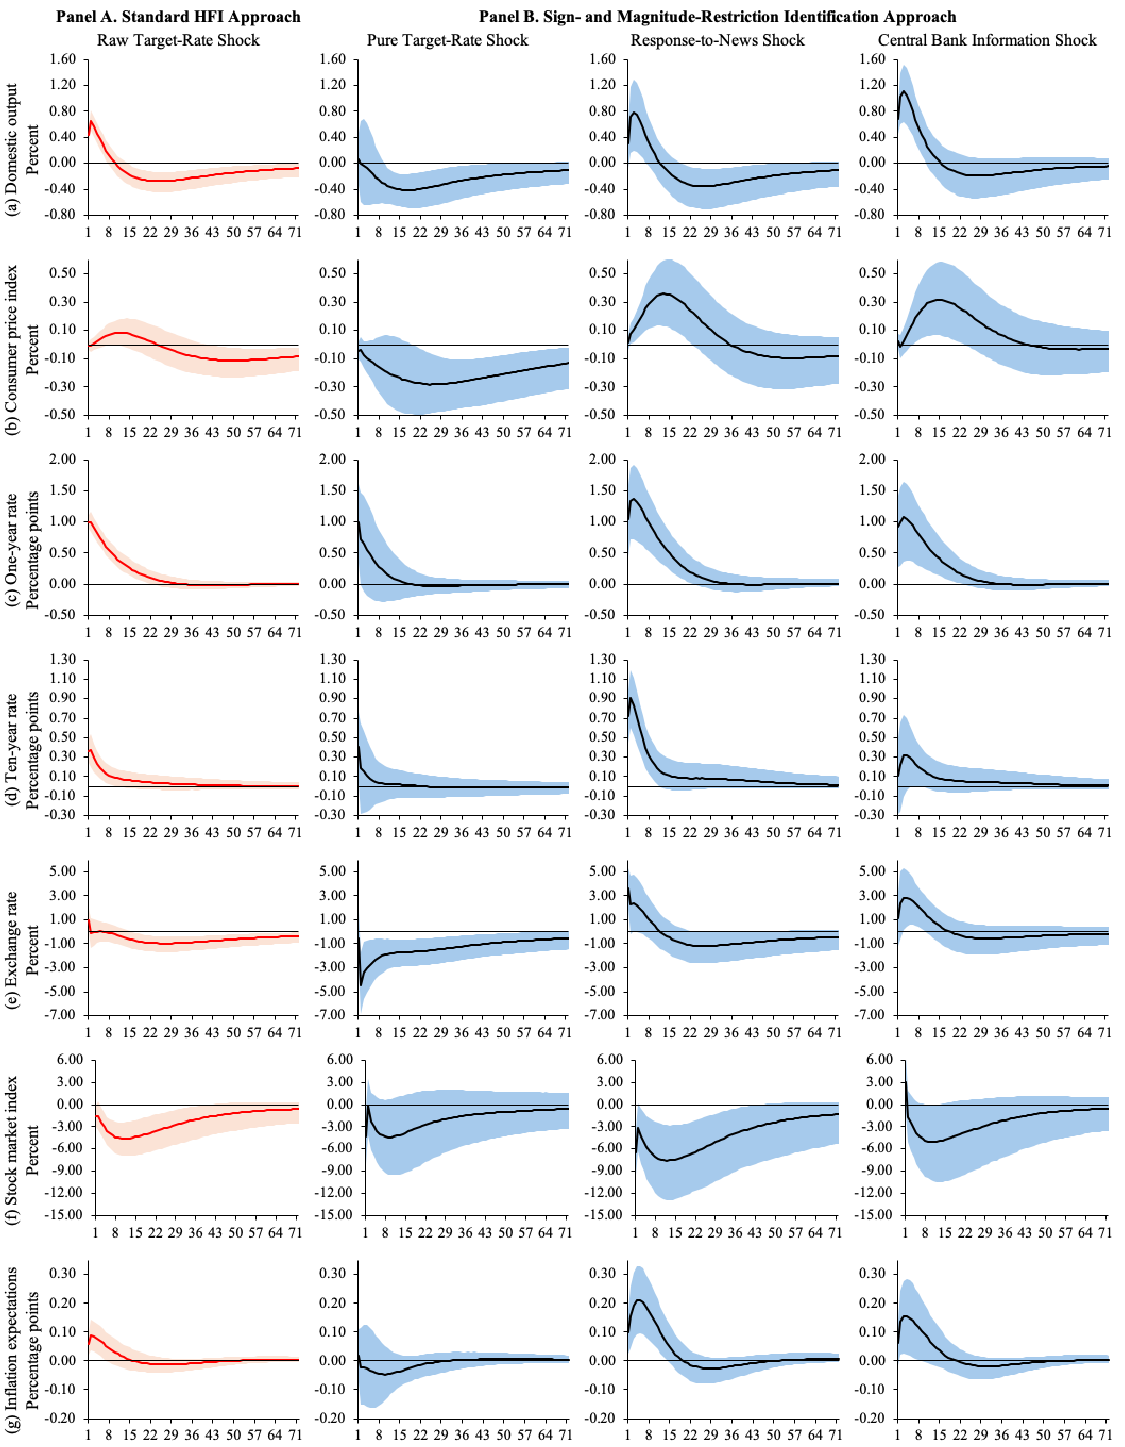
\includegraphics[width=\linewidth]{TR-2024m12-sincerores.pdf}
}
\caption[5pt]{Impulse Responses to MP, CBI, and RN shocks Disentangled from Target-Rate Surprises}
\end{center}
\begin{footnotesize} 
Notes: Responses  are  presented  for a 72-month horizon with the associated 68\% highest posterior density intervals (HPDIs). Target-rate shocks are normalized to imply a one percentage point increase in the one-year government bond yield. The CBI and RN shocks are scaled to match the magnitude of the normalized pure target-rate shock in standard deviation units.
\end{footnotesize} 
\end{figure}

Compared to the results in \hyperlink{Panel BF1}{Panel~A}, the contraction in output is substantially stronger and materializes earlier, with the peak decline occurring seven months sooner and reaching around 0.41\% below the baseline. A similar pattern emerges for prices, whose peak contraction is more than twice as pronounced (around 0.27\%) and occurs roughly two years after the disturbance—approximately half the time required in \hyperlink{Panel BF1}{Panel~A}. The exchange-rate response also changes markedly. Instead of the small and delayed appreciation observed following the raw disturbance, the Mexican peso now appreciates by approximately 4.25\% one month after the shock—a magnitude more than four times larger—before gradually returning toward its pre-shock level. Stock prices display a stronger impact response as well, declining by about 4.27\% compared to roughly 1.6\% after the unpurged shock. Finally, although both the one-year and ten-year government bond yields increase on impact, their responses appear less persistent than in \hyperlink{Panel BF1}{Panel~A}, suggesting that the tightening implied by the pure shock is shorter-lived and more consistent with a temporary policy adjustment. Overall, these estimates are more in line with the evidence reported by \hyperlink{Carrillo et al. (2025)}{Carrillo et al. (2025)} and \hyperlink{Deb et al. (2023)}{Deb et al. (2023)}, both in terms of magnitude and timing of the transmission mechanism.



We now describe the impulse responses to favorable CBI shocks reported in the third column of \hyperlink{Panel BF1}{Panel~B} of \hyperlink{Figure~1}{Figure~1}. In line with \hyperlink{Jarociński and Karadi (2025)}{Jarociński and Karadi (2020, 2025)}, favorable CBI shocks are followed by a persistent increase in the one-year government bond yield, an expansion in output, higher prices, and rising inflation expectations. Notably, the Mexican peso depreciates against the U.S.\ dollar in response to these shocks. Stock prices tend to rise on impact, while the ten-year government bond yield exhibits a positive, albeit muted, response. In particular, the depreciation of the domestic currency in response to favorable CBI shocks may be consistent with upward revisions in inflation expectations, as emphasized by \hyperlink{Gurkaynak et al. (2021)}{G\"urkaynak et al. (2021)} and \hyperlink{Stavrakeva and Tang (2019)}{Stavrakeva and Tang (2019)}.\footnote{An alternative explanation relates to Mexico’s tight integration with the United States. To the extent that the favorable information conveyed by the central bank is associated with positive spillovers from the U.S. economy—potentially accompanied by an appreciation of the U.S. dollar—then the estimated impulse responses may partly capture this external dollar-strength component, which would mechanically translate into a depreciation of the peso.}\textsuperscript{,}\footnote{While our findings are broadly consistent with U.S. evidence (\hyperlink{Pinchetti and Szczepaniak (2024)}{Pinchetti and Szczepaniak, 2024}; \hyperlink{Gründler et al. (2023)}{Gr\"undler et al., 2023}; \hyperlink{Stavrakeva and Tang (2019)}{Stavrakeva and Tang, 2019}), evidence from the euro area suggests a different pattern: favorable CBI shocks are associated with an appreciation of the domestic currency (\hyperlink{Kerssenfischer (2022)}{Kerssenfischer (2022)}).}  At the same time, the muted response of the ten-year government bond yield following a favorable CBI shock may reflect an offsetting mechanism. The stimulative effects of favorable information about economic fundamentals may reduce the term premium, thereby counteracting the upward pressure on long-term rates induced by the policy tightening.\footnote{The term premium is the additional compensation that investors require for holding longer-term instruments instead of rolling over short-term debt. According to \hyperlink{Carrillo et al. (2020)}{Carrillo et al. (2020)}, the response of the term premium depends on whether the information conveyed by the announcement is perceived as negative or positive for the economic outlook. The term premium tends to rise when news signals a deterioration in fundamentals and to fall when news points to a more favorable outlook.}

Taken together, these responses are consistent with an interpretation in which the central bank reveals favorable information about economic fundamentals while simultaneously tightening policy to lean against emerging overheating and inflationary pressures. Such pressures may operate through an aggregate demand channel and/or through exchange-rate pass-through effects. The persistent increase in the one-year government bond yield is consistent with a systematic policy response aimed at containing these pressures. While the tightening does not fully offset the initial expansionary effects of the news, it gradually neutralizes them over the medium term.

We now describe the impulse responses to hawkish RN shocks reported in the second column of \hyperlink{Panel BF1}{Panel~B} of \hyperlink{Figure~1}{Figure~1}. These shocks are followed by increases in interest rates, an expansion in output, higher prices, rising inflation expectations, and a depreciation of the domestic currency. These dynamics closely resemble those observed following favorable CBI shock and are consistent with the findings of \hyperlink{Bauer and Swanson (2023a, 2023b)}{Bauer and Swanson (2023a, 2023b)}. Overall, they may reflect a scenario in which the central bank tightens policy more aggressively than markets had anticipated in response to improving economic conditions or perceived upside risks to inflation. As in the CBI case, the tightening does not fully offset the expansionary effects associated with the underlying fundamentals but instead gradually neutralizes them over the medium term. 

Overall, these findings underscore the importance of disentangling MP shocks from their informational components. When target-rate surprises are treated as exogenous innovations, the resulting impulse responses may appear attenuated, delayed, or even puzzling, thereby obscuring the transmission mechanism of a conventional tightening. Once RN and CBI components are  isolated, the estimated effects of target-rate shocks become more consistent with standard theoretical predictions. In the next section, we apply the same decomposition framework to FG surprises, where distinguishing between policy and informational channels appears to be similarly important.




\subsection{Macroeconomic Effects of MP, RN, and CBI Shocks Disentangled from FG Surprises}

This section analyzes the macroeconomic effects of MP, CBI, and RN shocks extracted from FG surprises. As in the previous section, we present impulse responses under two identification approaches. The first corresponds to the \emph{standard HFI} approach, which treats the FG surprise as an exogenous MP shock and does not separately identify RN and CBI components. The second relies on a sign- and magnitude-restriction identification strategy that disentangles MP, RN, and CBI shocks from FG surprises. MP shocks identified under both approaches are normalized to correspond to a one percentage point increase in the one-year government bond yield. CBI and RN shocks are scaled to match the size of the normalized pure MP shock in standard deviation units.\footnote{\hyperlink{Figure B.24}{Figure~B.24} of \hyperlink{Appendix B}{Appendix~B} reports impulse responses without standardization.} The corresponding impact responses of the high-frequency surprises are reported in \hyperlink{Table 4}{Table~4}.

\begin{table}[t]
\hypertarget{Panel AT3}{}
\hypertarget{Panel BT3}{}
\hypertarget{Table 3}{}
\begin{center}
\resizebox{16cm}{!} {
\begin{tabular}{c c c c c c c c c}
\toprule
& \multicolumn{2}{c}{Panel A. Standard HFI}
& \multicolumn{6}{c}{Panel B. Sign- and Magnitude-Restriction Identification} \\
\cmidrule(lr){2-3}\cmidrule(lr){4-9}
High Frequency
& \multicolumn{2}{c}{FG Shock}
& \multicolumn{2}{c}{Pure FG Shock}
& \multicolumn{2}{c}{RN Shock}
& \multicolumn{2}{c}{CBI Shock} \\
\cmidrule(lr){2-3}\cmidrule(lr){4-5}\cmidrule(lr){6-7}\cmidrule(lr){8-9}
Surprise
& Mean & ($16^{pct}$, $84^{pct}$)
& Mean & ($16^{pct}$, $84^{pct}$)
& Mean & ($16^{pct}$, $84^{pct}$)
& Mean & ($16^{pct}$, $84^{pct}$) \\
\midrule
FG surprise
& 1.06 & (1.01, 1.10)
&  & 
&   & 
&   &  \\
RES
&  & 
& 1.47 & (1.02, 1.73)
& -0.24 & (-0.87, 0.46)
& 0.73 & (0.12, 1.41) \\
FIT
&   & 
& -0.12 & (-0.35, 0.14)
& 0.55 & (0.36, 0.65)
& 0.33 & (0.07, 0.58) \\
Stock market surprise
&   & 
& -4.40 & (-6.93, -1.57)
& -4.02 & (-6.51, -1.24)
& 5.69 & (2.95, 7.88) \\
\bottomrule
\end{tabular}}
\caption{Impact Responses of FG and Stock Market Surprises}
\end{center}
\begin{footnotesize}
\textit{Notes:} Posterior means and 16th and 84th percentiles. Units are percentage points. RES and FIT denote the residual and fitted components of the FG surprise, respectively. FG shocks identified under both approaches are normalized to correspond to a one percentage point increase in the one-year government bond yield. CBI and RN shocks are scaled to match the size of the normalized pure FG shock in standard deviation units.
\end{footnotesize}
\end{table}





\hyperlink{Panel BF1}{Panel~A} of \hyperlink{Figure~2}{Figure~2} displays in red impulse responses to a contractionary FG shock identified without disentangling RN and CBI components. For comparison, we also report in green the impulse responses to a contractionary pure target-rate shock, normalized to a one percentage point increase in the one-year government bond yield. The impulse responses to FG shocks do not appear to exhibit a clear attenuation bias potentially arising from RN and CBI components, with the possible exception of inflation expectations, which tend to rise in the short run. Compared with target-rate shocks, however, unpurged FG shocks are associated with a disproportionately large and more immediate contraction in domestic activity. Output declines by around 0.44\% one month after the shock, whereas the peak contraction following a pure target-rate shock (around 0.41\%) occurs only after about 19 months. Stock prices also appear to respond  more strongly following unpurged FG shocks. While these results could point to a more important role for FG in shaping macroeconomic outcomes, they may also reflect the amplification associated with the \emph{FG puzzle} discussed in the theoretical literature (see \hyperlink{Del Negro et al. (2023)}{Del Negro et al., 2023}), whereby revisions in expectations about the future policy path can generate macroeconomic effects that are disproportionately large relative to those of conventional MP shocks. At the same time, the relatively rapid response of output contrasts with the conventional view that monetary policy affects real activity with substantial lags.

\begin{figure}[t]
\hypertarget{Figure 2}{}
\hypertarget{Panel AF2}{}
\hypertarget{Panel BF2}{}
\begin{center}
\resizebox{13.5cm}{!} {
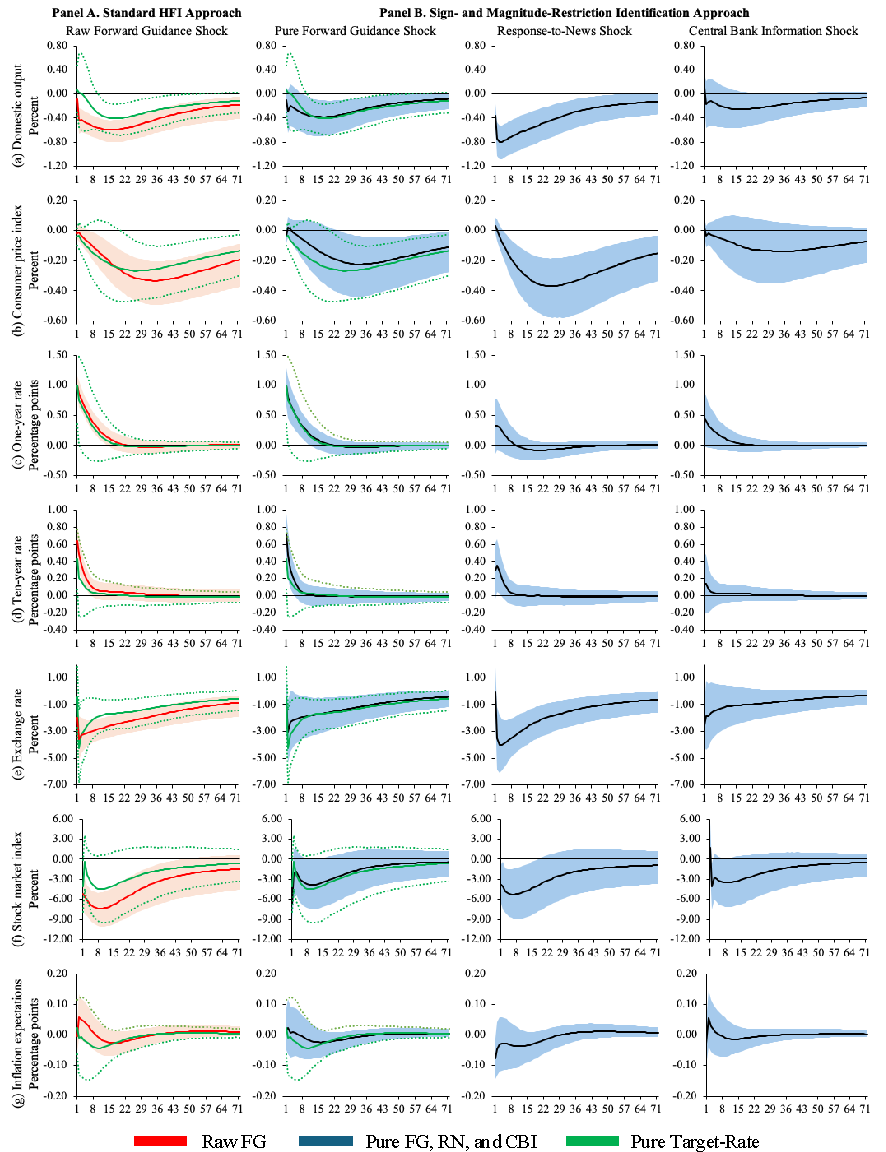
\includegraphics[width=\linewidth]{FG-2024m12_conTR-sincerores.pdf}
}
\caption[5pt]{Impulse Responses to MP, CBI, and RN shocks Disentangled from FG Surprises}
\end{center}
\begin{footnotesize} 
Notes: Responses  are  presented  for a 72-month horizon with the associated 68\% highest posterior density intervals (HPDIs). FG and target-rate shocks are normalized to imply a one percentage point increase in the one-year government bond yield. The CBI and RN shocks are scaled to match the magnitude of the normalized pure FG shock in standard deviation units.
\end{footnotesize} 
\end{figure}
 

\hyperlink{Panel BF1}{Panel~B} of \hyperlink{Figure~2}{Figure~2} reports impulse responses to the different structural components disentangled from FG surprises. As before, we also plot in green the impulse responses to a contractionary pure target-rate shock. As shown in the first column, once RN and CBI components are isolated, the effects of FG shocks become more moderate and closely resemble those following target-rate shocks. This is reflected in the substantial overlap between their impulse responses. Notably, the disproportionately large and almost immediate decline in output estimated under the standard HFI approach largely disappears. In addition, inflation expectations exhibit a more muted response and appear to be better anchored after the shock. These results are more consistent with the evidence reported by \hyperlink{Solis (2023b)}{Solís (2023b)}, who shows that FG surprises play an equally important role as target-rate surprises in the transmission of monetary policy to financial markets in Mexico. They also broadly align with the international evidence reported by \hyperlink{Andrade and Ferroni (2021)}{Andrade and Ferroni (2021)} and \hyperlink{Swanson (2021, 2024)}{Swanson (2021, 2024)}, who find that FG shocks tend to generate macroeconomic effects comparable to those of conventional policy shocks.

In general, the impulse responses to CBI and RN shocks identified from FG surprises do not differ markedly from those of pure FG shocks, as shown in \hyperlink{Panel BF1}{Panel~B} of \hyperlink{Figure~2}{Figure~2}. One aspect worth highlighting, however, is the behavior of inflation expectations, which tend to increase in the short run following a favorable CBI shock and may thus help explain their tendency to rise in response to unpurged FG shocks. This contrasts with the results for conventional MP shocks and suggests that attenuation bias operating through CBI and RN channels is likely limited in the case of FG. One possible interpretation is that the central bank responds to evolving demand conditions primarily through adjustments in the policy rate rather than through communication about the future policy path. This behavior may reflect the fact that, in EMEs, FG has typically been used as a complementary rather than a primary policy tool. Unlike in AEs—where central banks were constrained by the effective lower bound and relied more heavily on this unconventional tool—FG in EMEs tends to reinforce and complement policy rate decisions, rather than substitute for them. As a result, CBI and RN shocks may play a more prominent role in attenuating the effects of target-rate surprises than those of FG surprises.

Another aspect worth highlighting is the response of domestic output to hawkish RN shocks identified from FG surprises. The dynamics closely resemble those following unpurged FG shocks, suggesting that the amplified and rapid effects of such shocks on economic activity partly reflect RN contamination. One plausible interpretation is that, in the context of FG, market participants tend to overestimate the central bank’s reaction function. For instance, when economic activity is weakening, investors may anticipate a strongly accommodative policy path, whereas the central bank—consistent with the behavior discussed above and its primary mandate of price stability—signals a relatively more hawkish stance or provides little additional guidance due to concerns about inflationary pressures. The resulting impulse responses would then reflect both the contractionary effects of an upward revision in the expected path of policy rates and underlying weakness in output that was already underway, thereby generating disproportionately large and front-loaded declines in activity.


These findings highlight the importance of disentangling FG surprises into their structural components. While the standard HFI approach suggests that FG shocks exert large and front-loaded effects, isolating RN and CBI components reveals a more moderate transmission that more closely resembles that of conventional MP shocks. In addition, inflation expectations exhibit a more muted response and appear to remain better anchored following the unconventional policy shock. Importantly, regardless of the precise mechanism behind the amplified effects of unpurged FG shocks, disentangling their structural components helps mitigate these distortions and yields estimates that appear more consistent with standard transmission mechanisms, as well as with the empirical evidence documented by related studies.

\section{Conclusion}
\hypertarget{Section 6}{}

This paper studies the transmission of conventional and unconventional monetary policy in Mexico. Using high-frequency identification techniques, we distinguish between MP, CBI, and RN shocks embedded in two types of interest rate surprises around policy announcements: target-rate surprises, which capture unexpected changes in the current policy rate, and FG surprises, which reflect revisions to the expected future path of the policy rate. We then estimate the macroeconomic effects of these shocks using a monthly VAR.

We show that failing to disentangle CBI and RN components leads to biased estimates of monetary policy effects, giving rise to counterintuitive results such as expansions in output, rising prices, a depreciation of the domestic currency, and increases in inflation expectations following contractionary target-rate shocks. Once these components are isolated, these anomalies largely disappear. In response to contractionary pure target-rate shocks,  output and prices exhibit a hump-shaped decline, the domestic currency appreciates, and inflation expectations remain well anchored. For unconventional policy, unpurged FG shocks appear to have disproportionately large and immediate effects on economic activity. In addition, inflation expectations tend to rise in response to contractionary FG shocks. Once CBI and RN components are removed, however, the effects of these shocks become more moderate and closely resemble those of pure target-rate shocks. We also show that CBI and RN shocks play distinct contamination roles across policy instruments. While both tend to reverse the effects of target-rate shocks, RN shocks disproportionately amplify and accelerate the transmission of FG shocks, whereas CBI shocks play a more limited role.

Overall, our results highlight the importance of disentangling interest rate surprises into their structural components when studying monetary policy transmission in EMEs with characteristics similar to those of Mexico. Ignoring CBI and RN components may lead to misleading conclusions about the effectiveness of monetary policy in these economies. Regardless of the precise mechanism behind the disproportionately large and more immediate effects of unpurged FG shocks on domestic output, disentangling RN components helps mitigate these distortions and yields estimates that are more consistent with standard transmission mechanisms and the empirical evidence documented in the literature.

Future research could extend this approach to other EMEs, subject to the availability of high-frequency financial data. In addition, further work could explore how the relative importance of MP, CBI, and RN shocks evolves over time. It would also be interesting to extend this framework to incorporate other forms of central bank communication, such as policy minutes, press conferences, and speeches. An additional research avenue would be to disentangle asset purchase program surprises, given that several EMEs implemented these programs for the first time during the COVID-19 crisis.

\label{sec:conclusion}


\newpage

\begin{thebibliography}{99}


\bibitem{} \hypertarget{Andrade and Ferroni (2021)}{} Andrade, P., and Ferroni, F. (2021). Delphic and odyssean monetary policy shocks: Evidence from the euro area. \textit{Journal of Monetary Economics} \textbf{117}, 816-832.

\bibitem{} \hypertarget{Aruoba et al. (2021)}{} 
Aruoba, S. B., Fernández, A., Guzmán, D., Pastén, E., and Saffie, F. (2021). Monetary policy surprises in chile: Measurement \& real effects. Central Bank of Chile, Working Paper.

\bibitem{} \hypertarget{Bancoa}{} Banco de México (2020a). Quarterly inflation report. July-September.

\bibitem{} \hypertarget{Bancoa}{} Banco de México (2020b). Quarterly inflation report. October-December.

\bibitem{} \hypertarget{Bauer and Swanson (2023a)}{} 
Bauer, M. D., and Swanson, E. T. (2023a). An alternative explanation for the "fed information effect". \textit{American Economic Review} \textbf{113}(3), 664-700.

\bibitem{} \hypertarget{Bauer and Swanson (2023b)}{} 
Bauer, M. D., and Swanson, E. T. (2023b). A reassessment of monetary policy surprises and high-frequency identification. \textit{NBER Macroeconomics Annual} \textbf{37}(1), 87-155.

\bibitem{} \hypertarget{Beauregard et al. (2024)}{}Beauregard, R., Christensen, J. H., Fischer, E., and Zhu, S. (2024). Inflation expectations and risk premia in emerging bond markets: Evidence from Mexico. \textit{Journal of International Economics} \textbf{151}, 103961.

\bibitem{} \hypertarget{Bianchi et al. (2023)}{} 
Bianchi, F., Gómez-Cram, R., Kind, T., and Kung, H. (2023). Threats to central bank independence: High-frequency identification with twitter. \textit{Journal of Monetary Economics} \textbf{135}, 37-54.

\bibitem{} \hypertarget{Bjørnland (2009)}{}Bjørnland, H. C. (2009). Monetary policy and exchange rate overshooting: Dornbusch was right after all. \textit{Journal of International Economics} \textbf{79}(1), 64-77.

\bibitem{} \hypertarget{Bolhuis et al. (2024)}{} 
Bolhuis, M. A., Das, S., and Yao, B. (2024). A new dataset of high-frequency monetary policy shocks. IMF Working Paper.

\bibitem{} \hypertarget{Breitenlechner et al. (2021)}{} 
Breitenlechner, M., Gründler, D., and Scharler, J. (2021). Unconventional monetary policy announcements and information shocks in the US. \textit{Journal of Macroeconomics}. \textbf{67}, 103283.

\bibitem{} \hypertarget{Campbell et al. (2012)}{} Campbell, J. R., Evans, C. L., Fisher, J. D., Justiniano, A., Calomiris, C. W., and Woodford, M. (2012). Macroeconomic effects of federal reserve forward guidance. \textit{Brookings Papers on Economic Activity} \textbf{42}(1), 1-80.

\bibitem{} \hypertarget{Canova (2005)}{} Canova, F. (2005). The transmission of US shocks to Latin America. \textit{Applied Econometrics} \textbf{20}(2), 229-251.



\bibitem{} \hypertarget{Capistran at al. (2019)}{}Capistrán, C., Chiquiar, D., and Hernández, J. R. (2019). Identifying Dornbusch's exchange rate overshooting with structural VECs: evidence from Mexico. \textit{61st issue (December 2019) of the International Journal of Central Banking}.

\bibitem{} \hypertarget{Capistran et al. (2010)}{} Capistrán, C., Constandse, C., and Ramos-Francia, M. (2010). Multi-horizon inflation forecasts using disaggregated data. \textit{Economic Modelling} \textbf{27}(3), 666-677.

\bibitem{} \hypertarget{Carrillo et al. (2020)}{} Carrillo, J. A., Elizondo, R., and Hernández-Román, L. G. (2020). Inquiry on the transmission of US aggregate shocks to Mexico: a SVAR approach. \textit{Journal of International Money and Finance} \textbf{104}, 1-24.

\bibitem{} \hypertarget{Carrillo et al. (2025)}{}Carrillo, J., Elizondo, R., Hernández-Román, L., Ibarra, R., and Quiroga, M. (2025). Monetary policy transmission in a small open economy
before and after the pandemic: the case of Mexico. Banco de México, mimeo.

\bibitem{} \hypertarget{Cieslak (2018)}{}
Cieslak, A. (2018). Short-rate expectations and unexpected returns in treasury bonds. \textit{The Review of Financial Studies} \textbf{31}(9), 3265-3306.

\bibitem{} \hypertarget{Dahlhaus et al. (2018)}{}
Dahlhaus, T., Hess, K., and Reza, A. (2018). International transmission channels of US quantitative easing: Evidence from Canada. \textit{Journal of Money, Credit and Banking} \textbf{50}(2-3), 545-563.

\bibitem{} \hypertarget{De Pooter et al. (2014)}{} 
De Pooter, M., Robitaille, P., Walker, I., and Zdinak, M. (2014). Are Long-Term Inflation Expectations Well Anchored in Brazil, Chile, and Mexico? \textit{International Journal of Central Banking} \textbf{10}(2), 337-400.

\bibitem{} \hypertarget{Deb et al. (2023)}{}Deb, M. P., Estefania-Flores, J., Firat, M., Furceri, D., and Kothari, S. (2023). Monetary policy transmission heterogeneity: cross-country evidence (WP/23/204). International Monetary Fund Working Papers.

\bibitem{} \hypertarget{Del Negro et al. (2023)}{} 
Del Negro, M., Giannoni, M., and Patterson, C. (2023). The forward guidance puzzle. \textit{Journal of Political Economy} \textbf{1}(1), 43-79.

\bibitem{} \hypertarget{Eichenbaum and Evans (1995)}{} 
Eichenbaum, M., and Evans, C. L. (1995). Some empirical evidence on the effects of shocks to monetary policy on exchange rates. \textit{The Quarterly Journal of Economics} \textbf{110}(4), 975-1009.


\bibitem{} \hypertarget{Elizondo (2012)}{}Elizondo, R. (2012). Estimaciones del PIB mensual basadas en el IGAE (No. 2012-11). Banco de México Working Paper.



\bibitem{} \hypertarget{Evgenidis and Fasianos (2023)}{} Evgenidis, A., and Fasianos, A. (2023). Modelling monetary policy’s impact on labour markets under Covid-19. \textit{Economics Letters} \textbf{230}, 111241.


\bibitem{} \hypertarget{Faust and Rogers (2003)}{} Faust, J., and Rogers, J. H. (2003). Monetary policy's role in exchange rate behavior. \textit{Journal of Monetary Economics} \textbf{50}(7), 1403-1424.


\bibitem{} \hypertarget{Fink (2015)}{} Fink, F., and Schüler, Y. S. (2015). The transmission of US systemic financial stress: Evidence for emerging market economies. \textit{Journal of International Money and Finance} \textbf{55}, 6-26.

\bibitem{} \hypertarget{Gambacorta et al. (2014)}{}
Gambacorta, L., Hofmann, B., and Peersman, G. (2014). The effectiveness of unconventional monetary policy at the zero lower bound: A cross‐country analysis. \textit{Journal of Money, Credit and Banking} \textbf{46}(4), 615-642.

\bibitem{} \hypertarget{Georgiadis (2016)}{} Georgiadis, G. (2016). Determinants of global spillovers from US monetary policy. \textit{Journal of International Money and Finance} \textbf{67}, 41-61.

\bibitem{} \hypertarget{Gertler and Karadi (2015)}{}Gertler, M., and Karadi, P. (2015). Monetary policy surprises, credit costs, and economic activity. \textit{American Economic Journal: Macroeconomics} \textbf{7}(1), 44-76.



\bibitem{} \hypertarget{Gomes et al. (2023)}{} 
Gomes, D., Iachan, F., Ruhe, A. P., and Santos, C. (2023). Monetary policy and labor markets in a developing economy. Working Paper.

\bibitem{} \hypertarget{Gründler et al. (2023)}{} Gründler, D., Mayer, E., and Scharler, J. (2023). Monetary policy announcements, information shocks, and exchange rate dynamics. \textit{Open Economies Review} \textbf{34}(2), 341-369.

\bibitem{} \hypertarget{Gurkaynak et al. (2005)}{} Gürkaynak, R. S., Sack, B., and Swanson, E. T. (2005). Do actions speak louder than words? The response of asset prices to monetary policy actions and statements. \textit{International Journal of Central Banking} \textbf{1}(1), 55-93.

\bibitem{} \hypertarget{Gurkaynak et al. (2021)}{} Gürkaynak, R. S., Kara, A. H., Kısacıkoğlu, B., and Lee, S. S. (2021). Monetary policy surprises and exchange rate behavior. \textit{Journal of International Economics} \textbf{130}, 1-24.

\bibitem{} \hypertarget{Ibarra (2016)}{}Ibarra, R. (2016). How important is the credit channel in the transmission of monetary policy in Mexico? \textit{Applied Economics} \textbf{48}(36), 3462-3484.

\bibitem{} \hypertarget{Ilzetzki et al. (2019)}{}
Ilzetzki, E., Reinhart, C. M., and Rogoff, K. S. (2019). Exchange arrangements entering the twenty-first century: Which anchor will hold? \textit{The Quarterly Journal of Economics} \textbf{134}(2), 599-646.

\bibitem{} \hypertarget{JK (2020)}{} Jarociński, M., and Karadi, P. (2020). Deconstructing monetary policy surprises—the role of information shocks. \textit{American Economic Journal: Macroeconomics} \textbf{12}(2), 1-43.

\bibitem{} \hypertarget{Jarocinski and Karadi (2025)}{} 
Jarociński, M., and Karadi, P. (2025). Disentangling monetary policy, central bank information, and fed response to news shocks. CEPR Discussion Paper, 19923.

\bibitem{} \hypertarget{Kerssenfischer (2022)}{} Kerssenfischer, M. (2022). Information effects of euro area monetary policy. \textit{Economics Letters} \textbf{216}, 1-5.

\bibitem{} \hypertarget{Kim (2001)}{}Kim, S. (2001). International transmission of US monetary policy shocks: Evidence from VAR's. \textit{Journal of Monetary economics} \textbf{48}(2), 339-372.

\bibitem{} \hypertarget{Kim and Lim (2022)}{}Kim, S., and Lim, K. (2022). Effects of monetary policy shocks on exchange rate in emerging countries. \textit{The World Economy} \textbf{45}(4), 1242-1261.

\bibitem{} \hypertarget{Kim and Roubini (2000)}{}Kim, S., and Roubini, N. (2000). Exchange rate anomalies in the industrial countries: A solution with a structural VAR approach. \textit{Journal of Monetary economics} \textbf{45}(3), 561-586.





\bibitem{} \hypertarget{Kuttner (2001)}{} Kuttner, K. N. (2001). Monetary policy surprises and interest rates: Evidence from the Fed funds futures market. \textit{Journal of Monetary Economics} \textbf{47}(3), 523-544.

\bibitem{} \hypertarget{Litterman (1979)}{} Litterman, R.B., 1979. Techniques of forecasting using vector autoregressions. Federal Reserve Bank of Minneapolis, Working Paper 115.

\bibitem{} \hypertarget{MacDonald and Popiel (2020)}{}
MacDonald, M., and Popiel, M. K. (2020). Unconventional monetary policy in a small open economy. \textit{Open Economies Review} \textbf{31}, 1061-1115.


\bibitem{} \hypertarget{Miranda-Agrippino and Ricco (2021)}{} 
Miranda-Agrippino, S., and Ricco, G. (2021). The transmission of monetary policy shocks. \textit{American Economic Journal: Macroeconomics} \textbf{13}(3), 74-107.

\bibitem{} \hypertarget{Ng (2021)}{} 
Ng, S. (2021). Modeling macroeconomic variations after COVID-19 (No. w29060). National Bureau of Economic Research.

\bibitem{} \hypertarget{Pinchetti and Szczepaniak (2024)}{} 
Pinchetti, M., and Szczepaniak, A. (2024). Global Spillovers of the Fed Information Effect \textit{IMF Economic Review} \textbf{72}(2), 773-819.

\bibitem{} \hypertarget{Plagborg (2021)}{} 
Plagborg‐Møller, M., and Wolf, C. K. (2021). Local projections and VARs estimate the same impulse responses. \textit{Econometrica} \textbf{89}(2), 955-980.

\bibitem{} \hypertarget{Ramey (2016)}{}Ramey, V. A. (2016). Macroeconomic shocks and their propagation. \textit{Handbook of macroeconomics} \textbf{2}, 71-162.

\bibitem{} \hypertarget{Rogers et al. (2018)}{} 
Rogers, J. H., Scotti, C., and Wright, J. H. (2018). Unconventional monetary policy and international risk premia. \textit{Journal of Money, Credit and Banking} \textbf{50}(8), 1827-1850.

\bibitem{} \hypertarget{Romer and Romer (2000)}{} 
Romer, C., and Romer, D. (2000). Federal Reserve information and the behavior of interest rates. \textit{American Economic Review} \textbf{90}(3), 429-457.

\bibitem{} \hypertarget{Rubio-Ramirez et al. (2010)}{} Rubio-Ramirez, J. F., Waggoner, D. F., and Zha, T. (2010). Structural vector autoregressions: Theory of identification and algorithms for inference. \textit{The Review of Economic Studies} \textbf{77}(2), 665-696.

\bibitem{} \hypertarget{Scholl and Uhlig (2008)}{} Scholl, A., and Uhlig, H. (2008). New evidence on the puzzles: Results from agnostic identification on monetary policy and exchange rates. \textit{ournal of International Economics} \textbf{76}(1), 1-13.


\bibitem{} \hypertarget{Sims and Zha (1999)}{} 
Sims, C. A., and Zha, T. (1999). Error bands for impulse responses. \textit{Econometrica} \textbf{67}(5), 1113-1155

\bibitem{} \hypertarget{Solis (2023a)}{}Solís, P. (2023a). Does the exchange rate respond to monetary policy in Mexico? Solving an exchange rate puzzle in emerging markets. \textit{Journal of Money, Credit and Banking} \textbf{55}(8), 2093-2113.

\bibitem{} \hypertarget{Solis (2023b)}{}Solís, P. (2023b). Do central bank words matter in emerging markets? Evidence from Mexico. \textit{Journal of Macroeconomics} \textbf{78}, 1-16.

\bibitem{} \hypertarget{Stavrakeva and Tang (2019)}{} 
Stavrakeva, V., and Tang, J. (2019). The dollar during the great recession: US monetary policy signaling and the flight to safety. CEPR Discussion Paper, DP14034.


\bibitem{} \hypertarget{Stock and Watson (2002)}{}Stock, J. H., and Watson, M. W. (2002). Macroeconomic forecasting using diffusion indexes. \textit{Journal of Business \& Economic Statistics} \textbf{}\textbf{20}(2), 147-162.

\bibitem{} \hypertarget{Swanson (2021)}{} 
Swanson, E. T. (2021). Measuring the effects of federal reserve forward guidance and asset purchases on financial markets. \textit{Journal of Monetary Economics} \textbf{118}, 32-53.

\bibitem{} \hypertarget{Swanson (2024)}{} 
Swanson, E. T. (2024). The Macroeconomic Effects of the Federal Reserve’s Conventional and Unconventional Monetary Policies. \textit{IMF Economic Review} \textbf{72}(3), 1152-1184.

\bibitem{} \hypertarget{Swanson and Williams (2014)}{} Swanson, E. T., and Williams, J. C. (2014). Measuring the effect of the zero lower bound on medium-and longer-term interest rates. \textit{American Economic Review} \textbf{104}(10), 3154-3185.

\bibitem{} \hypertarget{Uhlig (2005)}{} Uhlig, H. (2005). What are the effects of monetary policy on output? Results from an agnostic identification procedure. \textit{Journal of Monetary Economics} \textbf{52}(2), 381-419.

\bibitem{} \hypertarget{Witheridge (2024)}{} 
Witheridge, W. (2024). Monetary policy and fiscal-led inflation in emerging markets. JMP NYU University, 1.

\bibitem{} \hypertarget{Wu and Xia (2016)}{} Wu, J. C., and Xia, F. D. (2016). Measuring the macroeconomic impact of monetary policy at the zero lower bound. \textit{Journal of Money, Credit and Banking} \textbf{48}(2-3), 253-291.

\end{thebibliography}
%TC:ignore
\newpage

\appendix

\section{Appendix: Bayesian estimation}
\setcounter{equation}{0}
\hypertarget{Appendix A}{}

We estimate the VAR at the monthly frequency with a vector of high-frequency surprises and domestic macroeconomic and financial variables, together with exogenous foreign controls.

\paragraph{Reduced form.}
Let the vector of endogenous variables be given by
\[
\boldsymbol{Y}_t =
\begin{pmatrix}
\boldsymbol{m}_t^{\,j} \\
\boldsymbol{y}_t
\end{pmatrix},
\qquad j \in \{\text{TR}, \text{FG}\},
\]
where $\boldsymbol{m}_t^{\,j} \in \mathbb{R}^{N_m}$ collects the fitted and residual components $(\text{FIT}_t^{\,j}, \text{RES}_t^{\,j})$ associated with either target-rate or forward-guidance surprises, together with the equity-price surprise $\text{SP}_t$, and $\boldsymbol{y}_t \in \mathbb{R}^{N_y}$ stacks domestic macroeconomic and financial variables. The vector $\boldsymbol{Z}_t \in \mathbb{R}^{N_z}$ collects exogenous foreign controls.

The VAR is specified as
\begin{equation}
\label{eq:A1_VAR}
\boldsymbol{Y}_t
=
\boldsymbol{c}
+ \sum_{p=1}^{P}
\boldsymbol{B}^{p}\,\boldsymbol{Y}_{t-p}
+ \boldsymbol{\delta}\,\boldsymbol{Z}_t
+ \boldsymbol{u}_t,
\qquad
\boldsymbol{u}_t \sim \mathcal{N}(\mathbf{0}, \boldsymbol{\Sigma}).
\end{equation}

\paragraph{Stacked representation.}
Let $\boldsymbol{Y} = (\boldsymbol{Y}_1,\dots,\boldsymbol{Y}_T)^\prime$ and define the regressor matrix $\boldsymbol{X}$ such that a typical row is
\[
\boldsymbol{x}_t^\prime =
\big(\boldsymbol{Y}_{t-1}^\prime,\ldots,\boldsymbol{Y}_{t-P}^\prime,\ 1,\ \boldsymbol{Z}_t^\prime\big).
\]
Then the system can be written compactly as
\[
\boldsymbol{Y} = \boldsymbol{X}\boldsymbol{B} + \boldsymbol{U},
\]
where $\boldsymbol{B}$ collects all coefficient matrices, intercepts, and exogenous loadings.

\paragraph{Prior.}
We adopt an independent Normal–Inverse-Wishart prior, combining a Minnesota prior on lag coefficients with diffuse priors on intercepts and exogenous variables:
\begin{align}
p(\boldsymbol{\Sigma}\mid \underline{\boldsymbol{S}},\underline{\boldsymbol{v}})
&= \mathrm{IW}(\underline{\boldsymbol{S}},\underline{\boldsymbol{v}}),\\
p\!\left(\mathrm{vec}\,\boldsymbol{B}\mid \underline{\boldsymbol{B}},\underline{\boldsymbol{Q}}\right)
&= \mathcal{N}\!\left(\mathrm{vec}\,\underline{\boldsymbol{B}},\ \underline{\boldsymbol{Q}}\right).
\end{align}

The prior mean for the first own lag coefficient is set to one for output and prices and to zero for all other variables. All other lag coefficients are centered at zero. This choice has negligible effects on the posterior estimates and impulse responses. The prior standard deviation for the coefficient on lag $p$ of variable $j$ in equation $i$ is given by
\[
\mathrm{sd}\!\left(\beta_{i\leftarrow j,p}\right)=\lambda_1^{-1}\,\frac{\sigma_i}{\sigma_j}\,p^{-\lambda_2},
\qquad \lambda_1=5,\ \lambda_2=1,
\]
where $\sigma_i$ and $\sigma_j$ are residual standard deviations from univariate AR($P$) models.

We set $\underline{\boldsymbol{v}} = N + 2$, with $N = N_m + N_y$, and $\underline{\boldsymbol{S}} = \mathrm{diag}(\sigma_1^2,\ldots,\sigma_N^2)$. Coefficients on intercepts and exogenous variables receive diffuse priors.

\paragraph{Conditional posteriors.}
Let $\boldsymbol{U} = \boldsymbol{Y} - \boldsymbol{X}\boldsymbol{B}$. The conditional posterior distributions are given by
\begin{align}
p(\boldsymbol{\Sigma}\mid \boldsymbol{Y}, \boldsymbol{B})
&= \mathrm{IW}(\overline{\boldsymbol{S}}, \overline{\boldsymbol{v}}),\\
\overline{\boldsymbol{S}}
&= \boldsymbol{U}^\prime \boldsymbol{U} + \underline{\boldsymbol{S}},\qquad
\overline{\boldsymbol{v}} = T + \underline{\boldsymbol{v}}.
\end{align}

Conditional on $\boldsymbol{\Sigma}$, the posterior for $\boldsymbol{B}$ is
\begin{align}
p\!\left(\mathrm{vec}\,\boldsymbol{B}\mid \boldsymbol{Y}, \boldsymbol{\Sigma}\right)
&= \mathcal{N}\!\left(\mathrm{vec}\,\overline{\boldsymbol{B}},\ \overline{\boldsymbol{Q}}\right),\\
\overline{\boldsymbol{Q}}
&=\Big(\underline{\boldsymbol{Q}}^{-1}+\boldsymbol{\Sigma}^{-1}\otimes \boldsymbol{X}^\prime\boldsymbol{X}\Big)^{-1},\\
\mathrm{vec}\,\overline{\boldsymbol{B}}
&=\overline{\boldsymbol{Q}}\left[\underline{\boldsymbol{Q}}^{-1}\mathrm{vec}\,\underline{\boldsymbol{B}}
+\left(\boldsymbol{\Sigma}^{-1}\otimes \boldsymbol{X}^\prime\right)\mathrm{vec}(\boldsymbol{Y})\right].
\end{align}


\newpage
\section{Appendix: Supplemental Results}
\hypertarget{Appendix B}{}

\renewcommand{\thetable}{\thesection{}.1}
\begin{table}[htbp]
\hypertarget{Table B.1}{}
\begin{center}
\resizebox{0.58\textwidth}{!}{
\begin{tabular}{lcccc}
\toprule
 & \multicolumn{2}{c}{Target-rate surprise} & \multicolumn{2}{c}{FG surprise} \\
\cmidrule(lr){2-3} \cmidrule(lr){4-5}
 & Extended & Baseline & Extended & Baseline \\
\midrule

\multicolumn{5}{l}{\textbf{\emph{Domestic news}}} \\[0.2em]

$\Delta \log$ domestic output (6m)
& -0.037 & -0.036 
& 0.139 & 0.239 \\
& (0.193) & (0.177)
& (0.726) & (0.674) \\

$\Delta \log$ CPI (6m)
& -0.248 & -0.287 
& 1.985 & 2.109 \\
& (1.269) & (1.246)
& (3.289) & (3.483) \\

$\Delta \log$ Stock market index (3m)
& 0.036 & -- 
& 0.122 & -- \\
& (0.093) & 
& (0.230) & \\

$\Delta \log$ MXN/USD (3m)
& -0.010 & 0.007 
& 1.124** & 0.962** \\
& (0.191) & (0.168)
& (0.442) & (0.410) \\

$\Delta$ FX implied volatility (3m)
& 0.004* & 0.004* 
& -0.009** & -0.010** \\
& (0.002) & (0.002)
& (0.004) & (0.004) \\

$\Delta$ Interbank rate (3m)
& 0.014 & 0.022 
& -0.003 & -0.010 \\
& (0.027) & (0.015)
& (0.057) & (0.027) \\

$\Delta$ 2-year gov. yield (3m)
& 0.020 & 0.030* 
& 0.114 & 0.008 \\
& (0.024) & (0.015)
& (0.075) & (0.039) \\

$\Delta$ 10-year gov. yield (3m)
& 0.023 & -- 
& -0.136 & -- \\
& (0.042) & 
& (0.114) & \\

$\Delta$ Yield curve slope (3m)
& -0.018 & -- 
& 0.055 & -- \\
& (0.043) & 
& (0.093) & \\[0.4em]

\multicolumn{5}{l}{\textbf{\emph{External news}}} \\[0.2em]

$\Delta \log$ Industrial prod. (6m)
& -0.006 & 0.007 
& 0.718 & 0.782 \\
& (0.296) & (0.261)
& (0.881) & (0.849) \\

$\Delta \log$ US CPI (6m)
& 1.143 & 1.201 
& -1.596 & -1.219 \\
& (0.916) & (0.979)
& (1.913) & (2.053) \\

$\Delta \log$ S\&P 500 (3m)
& 0.152 & 0.129 
& -0.056 & 0.252 \\
& (0.171) & (0.143)
& (0.396) & (0.337) \\

$\Delta \log$ VIX (3m)
& 0.011 & -- 
& -0.034 & -- \\
& (0.025) & 
& (0.070) & \\

$\Delta$ 2-year Treasury yield (3m)
& -0.001 & -0.007 
& 0.042 & 0.091** \\
& (0.030) & (0.021)
& (0.068) & (0.040) \\

$\Delta$ 10-year Treasury yield (3m)
& -0.064* & -0.052* 
& 0.005 & -0.095* \\
& (0.038) & (0.026)
& (0.100) & (0.054) \\

$\Delta$ Yield curve slope (3m)
& 0.008 & -- 
& -0.030 & -- \\
& (0.023) & 
& (0.053) & \\

$\Delta \log$ Brent oil price (3m)
& 0.078* & 0.078* 
& 0.113 & 0.123 \\
& (0.044) & (0.045)
& (0.106) & (0.110) \\[0.4em]

\multicolumn{5}{l}{\textbf{\emph{Lagged monetary policy surprises}}} \\[0.2em]

Surprise$_{t-1}$
& 0.020 & 0.021 
& -0.276*** & -0.225** \\
& (0.123) & (0.120)
& (0.096) & (0.097) \\

Surprise$_{t-2}$
& -0.013 & -- 
& -0.120 & -- \\
& (0.087) & 
& (0.084) & \\

\midrule
$R^2$
& 0.227 & 0.224
& 0.195 & 0.154 \\

Adjusted $R^2$
& 0.151 & 0.173
& 0.115 & 0.099 \\

Observations
& 213 & 213
& 213 & 213 \\

\bottomrule
\end{tabular}}
\caption{Regressions of High-Frequency Monetary Policy Surprises on Macroeconomic and
Financial News: Extended vs.\ Baseline Specification}
\end{center}
\begin{footnotesize}
\textit{Notes}: The extended specification augments the baseline projection reported in Table~1 with a broader set of macro-financial controls. Variables not included in the baseline are denoted by ``--''. Standard errors (in parentheses) are heteroskedasticity- and autocorrelation-consistent (HAC), computed using a Newey--West estimator. $^{*}$, $^{**}$, and $^{***}$ denote significance at the 10\%, 5\%, and 1\% levels, respectively.
\end{footnotesize}
\end{table}

\renewcommand{\thefigure}{\thesection{}.1}
\begin{figure}[htbp]
\hypertarget{Figure B.1}{}
\hypertarget{Panel AF2}{}
\hypertarget{Panel BF2}{}
\begin{center}
\resizebox{11.5cm}{!} {
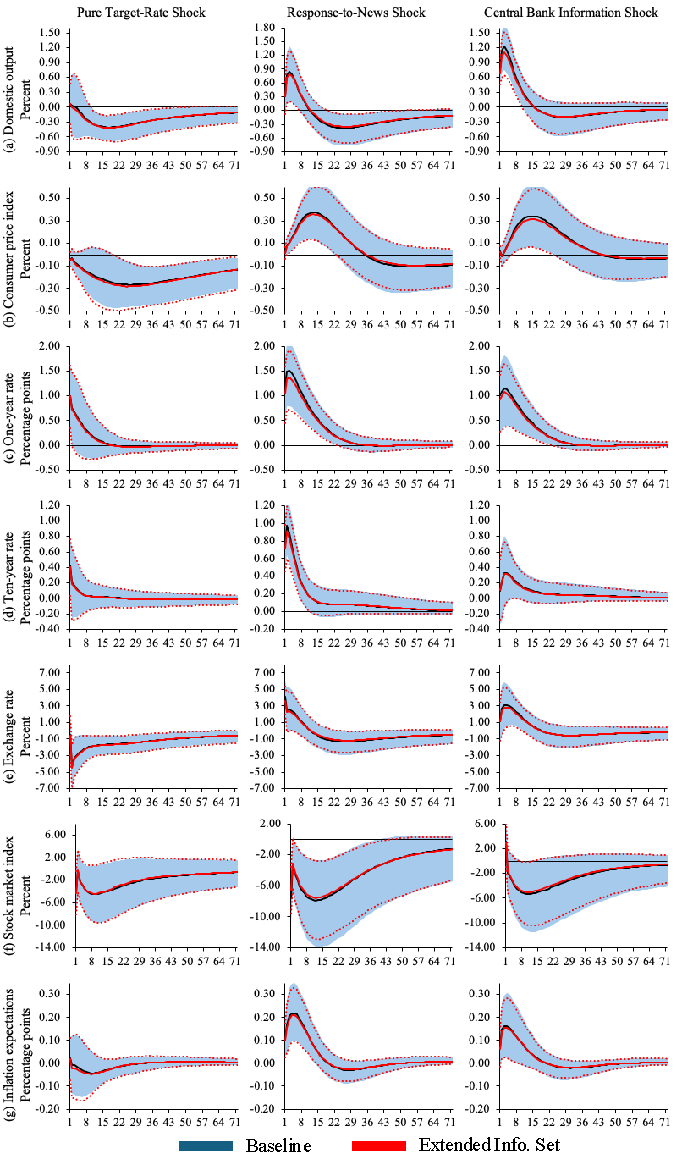
\includegraphics[width=\linewidth]{TR-Extended.pdf}
}
\caption[5pt]{Impulse Responses to Target-Rate, Response-to-News, and Central Bank Information Shocks: Baseline vs. Extended Information Set}
\end{center}
\begin{footnotesize} 
Notes: Responses  are  presented  for a 72-month horizon with the associated 68\% highest posterior density intervals (HPDIs).
\end{footnotesize} 
\end{figure}

\renewcommand{\thefigure}{\thesection{}.2}
\begin{figure}[htbp]
\hypertarget{Figure B.2}{}
\hypertarget{Panel AF2}{}
\hypertarget{Panel BF2}{}
\begin{center}
\resizebox{11.5cm}{!} {
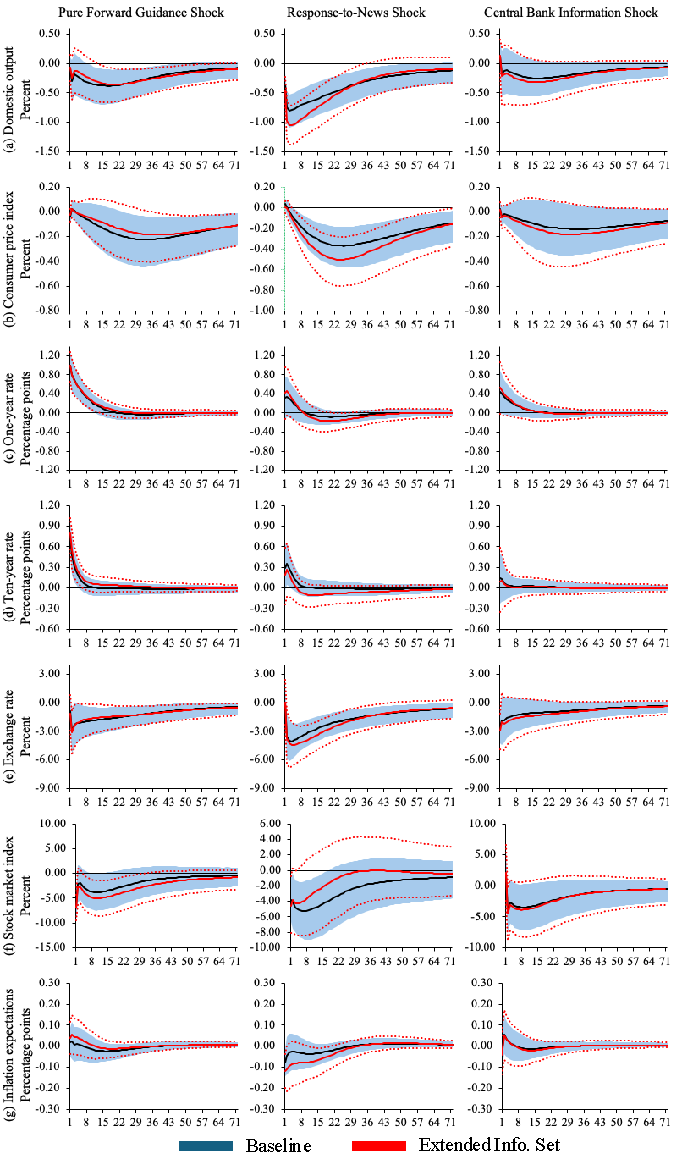
\includegraphics[width=\linewidth]{FG-Extended.pdf}
}
\caption[5pt]{Impulse Responses to Forward Guidance, Response-to-News, and Central Bank Information Shocks: Baseline vs. Extended Information Set}
\end{center}
\begin{footnotesize} 
Notes: Responses  are  presented  for a 72-month horizon with the associated 68\% highest posterior density intervals (HPDIs).
\end{footnotesize} 
\end{figure}

\renewcommand{\thetable}{\thesection{}.2}
\begin{table}[htbp]
\hypertarget{Table B.2}{}
\begin{center}
\resizebox{0.65\textwidth}{!}{
\begin{tabular}{lcc}
\toprule
Variable (baseline set) & Target-rate surprise & FG surprise \\
\midrule
Constant & -0.883 & -1.406 \\

\multicolumn{3}{l}{\textbf{\emph{Domestic news}}} \\[0.2em]
$\Delta \log$ domestic output (6m) & -- & -- \\
$\Delta \log$ CPI (6m) & -- & -- \\
$\Delta \log$ MXN/USD (3m) & -- & -- \\
$\Delta$ FX implied volatility (3m) & 0.001 & -0.004 \\
$\Delta$ Interbank rate (3m) & 0.020 & -- \\
$\Delta$ 2-year gov. yield (3m) & 0.013 & -- \\[0.4em]

\multicolumn{3}{l}{\textbf{\emph{External news}}} \\[0.2em]
$\Delta \log$ Industrial prod. (6m) & 0.020 & -- \\
$\Delta \log$ US CPI (6m) & 0.849 & -- \\
$\Delta \log$ S\&P 500 (3m) & -- & -- \\
$\Delta$ 2-year Treasury yield (3m) & -0.002 & -- \\
$\Delta$ 10-year Treasury yield (3m) & -0.009 & -- \\
$\Delta \log$ Brent oil price (3m) & 0.003 & -- \\[0.4em]

\multicolumn{3}{l}{\textbf{\emph{Lagged monetary policy surprises}}} \\[0.2em]
Surprise$_{t-1}$ & 0.005 & -0.038 \\

\midrule
Optimal $\lambda$ & 0.798 & 2.729 \\
Non-zero coefficients & 10 & 3 \\
$R^2$ & 0.162 & 0.056 \\
Observations & 213 & 213 \\
\bottomrule
\end{tabular}}
\caption{LASSO Selection over the Baseline Information Set}
\end{center}
\begin{footnotesize}
\textit{Notes}: This table reports LASSO (L1-penalized) projections estimated over the baseline information set used in Table~1, evaluated at the cross-validated optimal penalty parameter $\lambda$. Regressors are standardized prior to estimation. Variables not selected by the regularization procedure are denoted by ``--''.
\end{footnotesize}
\end{table}




\renewcommand{\thefigure}{\thesection{}.3}
\begin{figure}[htbp]
\hypertarget{Figure B.3}{}
\begin{center}
\resizebox{11.5cm}{!} {
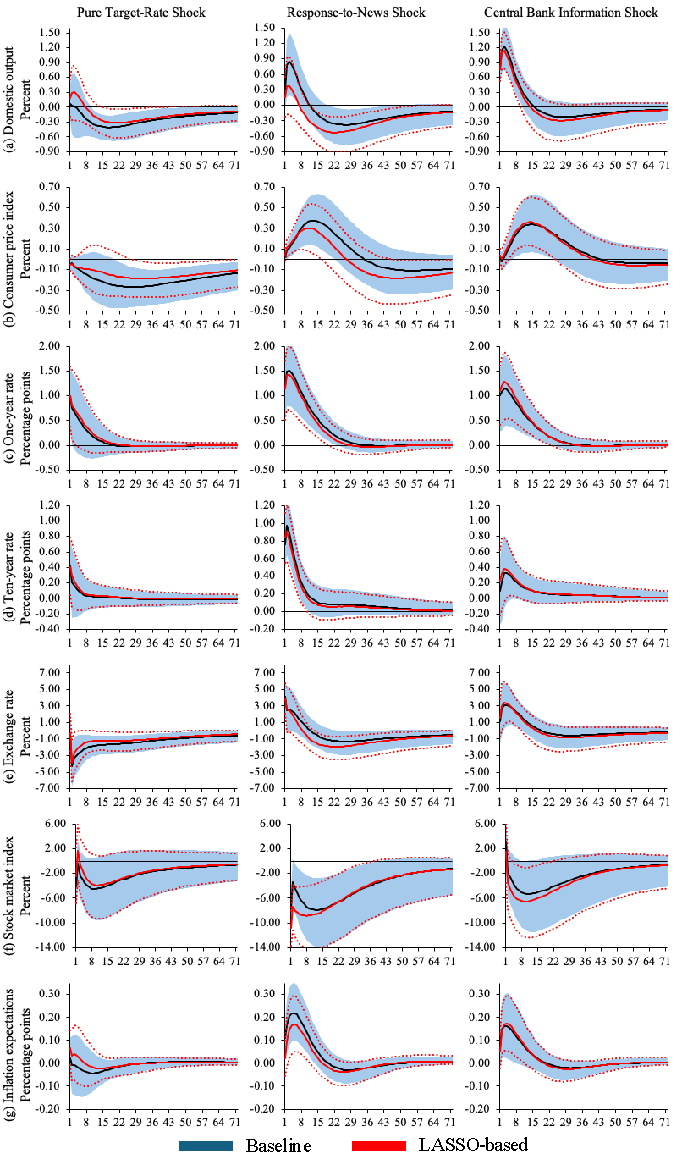
\includegraphics[width=\linewidth]{TR-Lasso.pdf}
}
\caption[5pt]{Impulse Responses to Target-Rate, Response-to-News, and Central Bank Information Shocks: Baseline vs. LASSO Diagnostic Projections}
\end{center}
\begin{footnotesize} 
Notes: Responses  are  presented  for a 72-month horizon with the associated 68\% highest posterior density intervals (HPDIs).
\end{footnotesize} 
\end{figure}

\renewcommand{\thefigure}{\thesection{}.4}
\begin{figure}[htbp]
\hypertarget{Figure B.4}{}
\begin{center}
\resizebox{11.5cm}{!} {
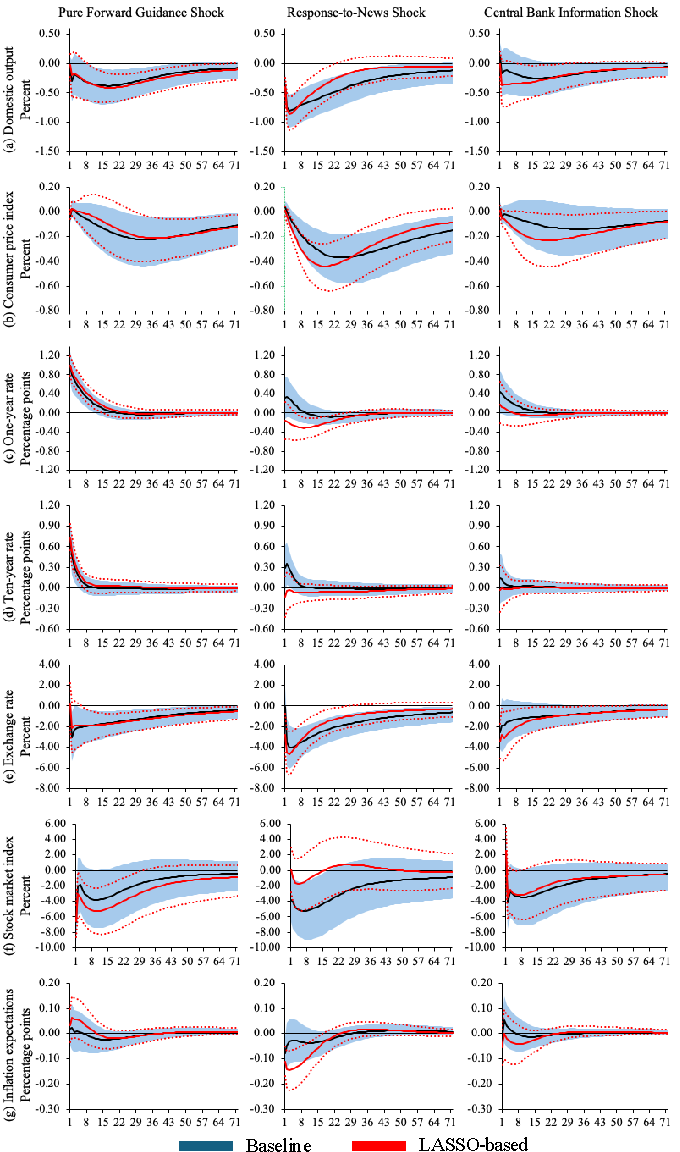
\includegraphics[width=\linewidth]{FG-Lasso.pdf}
}
\caption[5pt]{Impulse Responses to Forward Guidance, Response-to-News, and Central Bank Information Shocks: Baseline vs. LASSO Diagnostic Projections}
\end{center}
\begin{footnotesize} 
Notes: Responses  are  presented  for a 72-month horizon with the associated 68\% highest posterior density intervals (HPDIs).
\end{footnotesize} 
\end{figure}

\renewcommand{\thetable}{\thesection{}.3}
\begin{table}[H]
\begin{center}
\resizebox{0.5\textwidth}{!}{
\begin{tabular}{lc}
\toprule
 & Equity-price surprise \\
\midrule

\multicolumn{2}{l}{\textbf{\emph{External financial variables}}} \\[0.2em]

$\Delta \log$ S\&P 500  
& 0.493*** \\
& (0.061) \\

$\Delta \log$ VIX  
& 0.017* \\
& (0.010) \\

$\Delta$ 2-year Treasury yield 
& 0.029** \\
& (0.011) \\[0.4em]

Constant  
& $-$0.025 \\
& (0.057) \\[0.4em]

\midrule
$R^2$              & 0.300 \\
Adjusted $R^2$     & 0.290 \\
Observations       & 214   \\
\bottomrule
\end{tabular}}
\caption{Regression of Equity-Price Surprises on External Financial Variables}
\end{center}
\begin{footnotesize}
\textit{Notes}: This table reports coefficient estimates from a regression of equity-price surprises on external financial variables. Standard errors (in parentheses) are heteroskedasticity- and autocorrelation-consistent (HAC), computed using a Newey--West estimator. $^{*}$, $^{**}$, and $^{***}$ denote significance at the 10\%, 5\%, and 1\% levels, respectively.
\end{footnotesize}
\end{table}


\renewcommand{\thefigure}{\thesection{}.5}
\begin{figure}[htbp]
\hypertarget{Figure B.5}{}
\begin{center}
\resizebox{13cm}{!} {
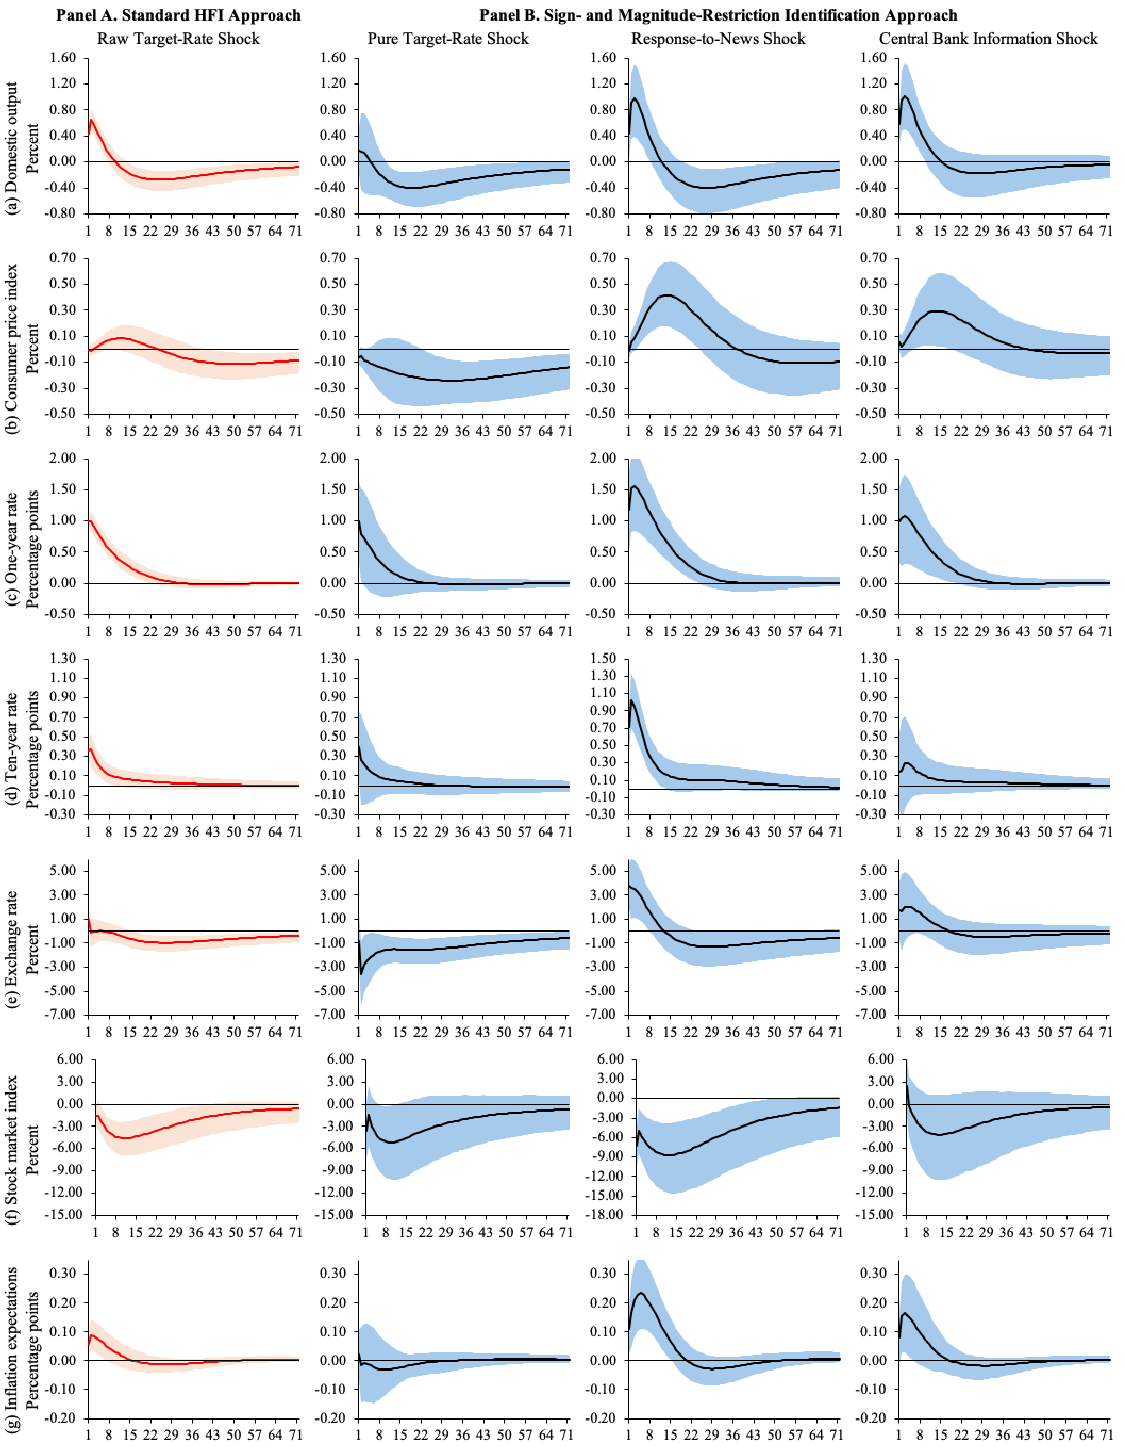
\includegraphics[width=\linewidth]{TR-IPCorto.pdf}
}
\caption[5pt]{Impulse Responses to Target-Rate, Response-to-News, and Central Bank Information Shocks: Specification using  Orthogonalized Equity-Price Surprise}
\end{center}
\begin{footnotesize} 
Notes: Responses  are  presented  for a 72-month horizon with the associated 68\% highest posterior density intervals (HPDIs).
\end{footnotesize} 
\end{figure}

\renewcommand{\thefigure}{\thesection{}.6}
\begin{figure}[htbp]
\hypertarget{Figure B.6}{}
\begin{center}
\resizebox{14cm}{!} {
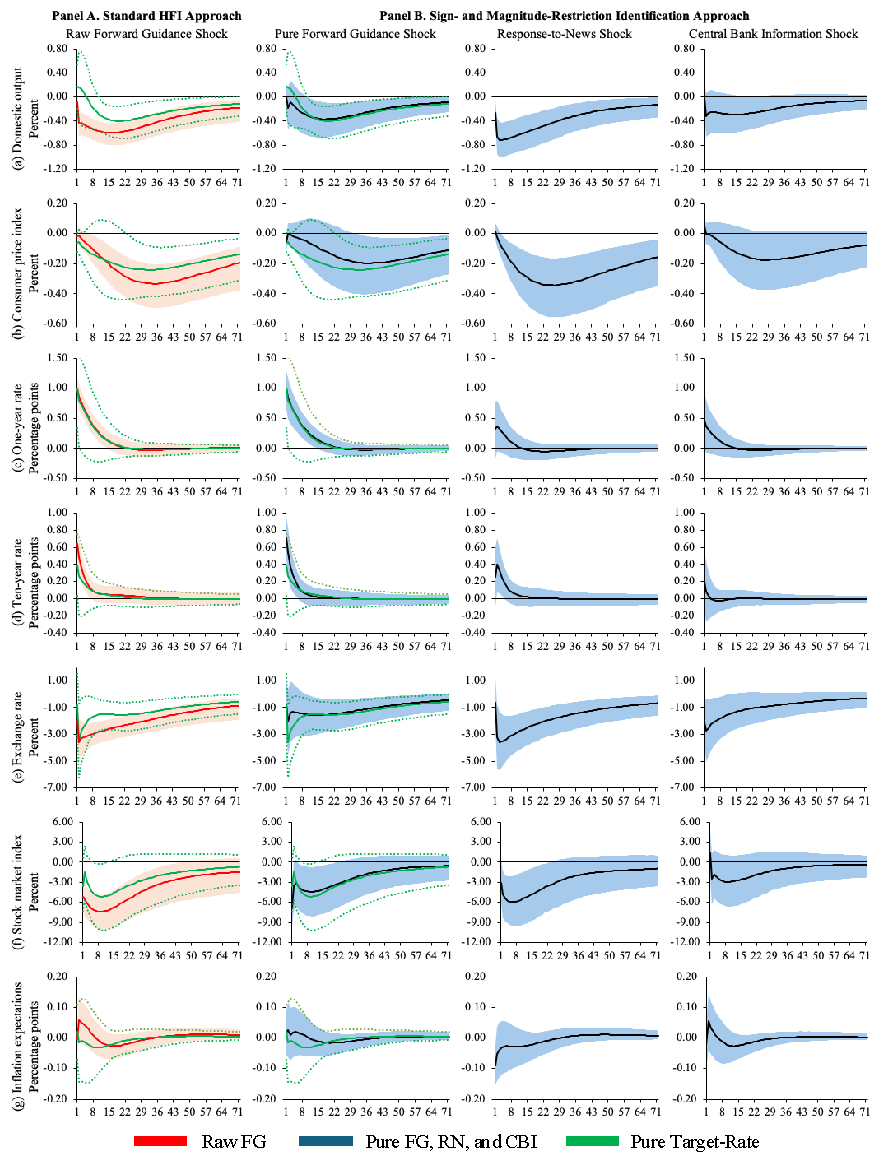
\includegraphics[width=\linewidth]{FG-IPCorto.pdf}
}
\caption[5pt]{Impulse Responses to Forward Guidance, Response-to-News, and Central Bank Information Shocks: Specification using  Orthogonalized Equity-Price Surprise}
\end{center}
\begin{footnotesize} 
Notes: Responses  are  presented  for a 72-month horizon with the associated 68\% highest posterior density intervals (HPDIs).
\end{footnotesize} 
\end{figure}

\renewcommand{\thefigure}{\thesection{}.7}
\begin{figure}[htbp]
\hypertarget{Figure B.7}{}
\begin{center}
\resizebox{13cm}{!} {
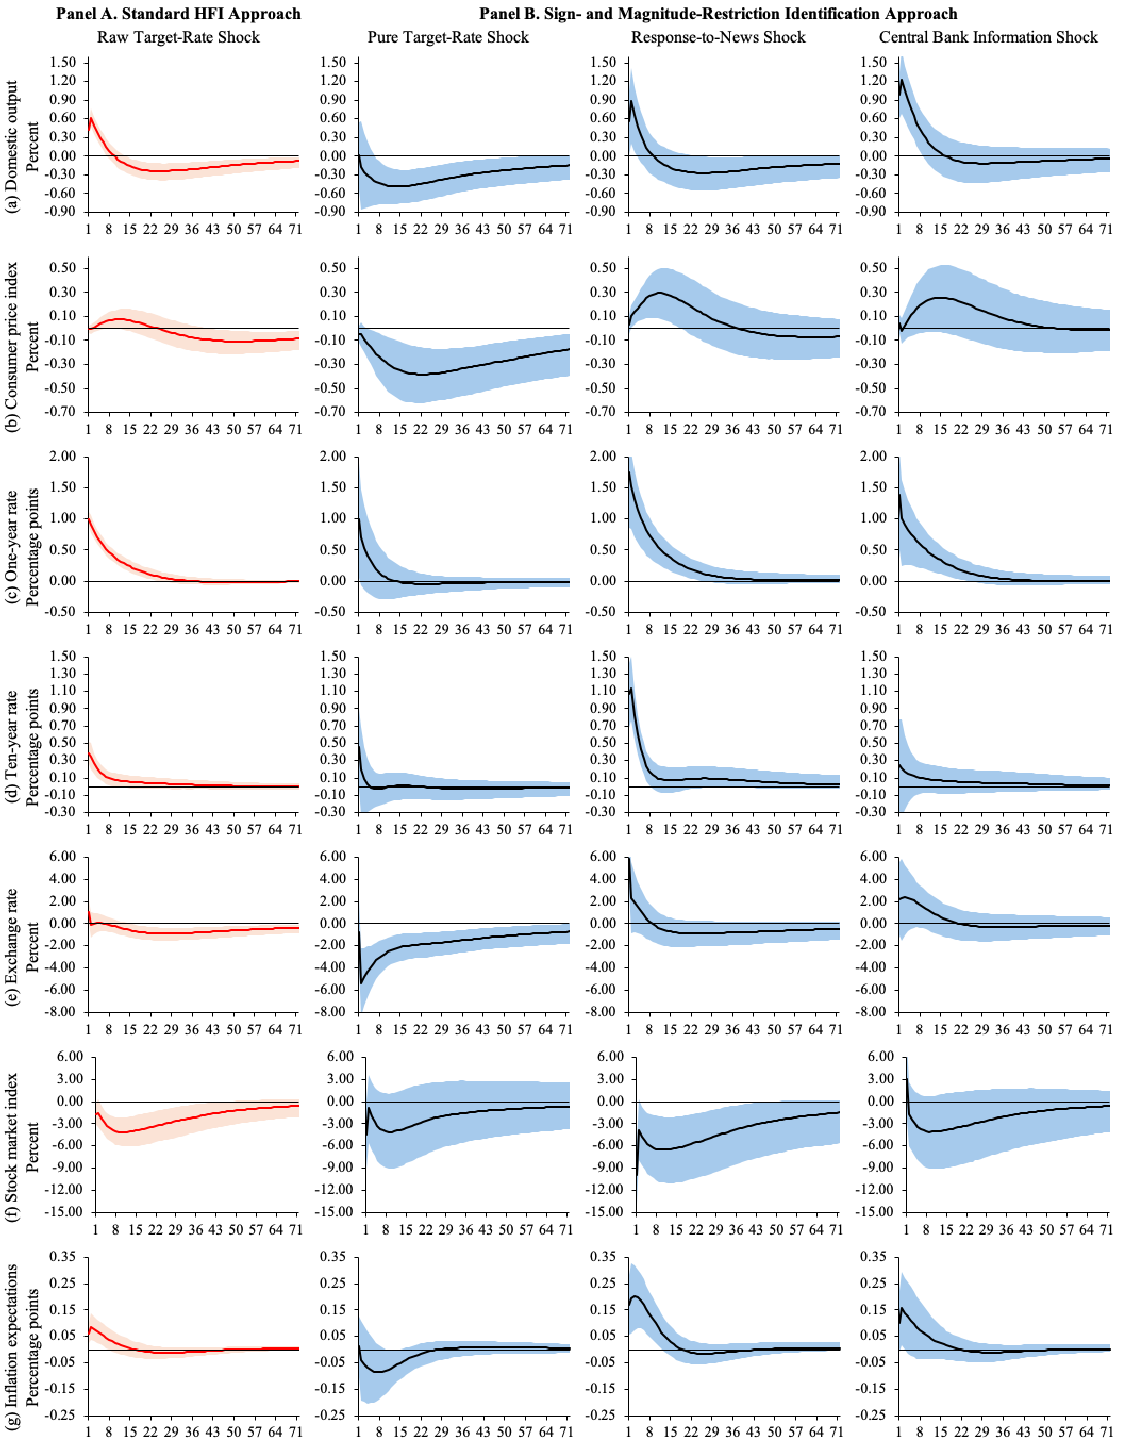
\includegraphics[width=\linewidth]{TR-cero.pdf}
}
\caption[5pt]{Impulse Responses to Target-Rate, RN, and CBI Shocks: Exogenous High-Frequency Block Specification}
\end{center}
\begin{footnotesize} 
Notes: Responses  are  presented  for a 72-month horizon with the associated 68\% highest posterior density intervals (HPDIs).
\end{footnotesize} 
\end{figure}



\renewcommand{\thefigure}{\thesection{}.8}
\begin{figure}[htbp]
\hypertarget{Figure B.8}{}
\begin{center}
\resizebox{14cm}{!} {
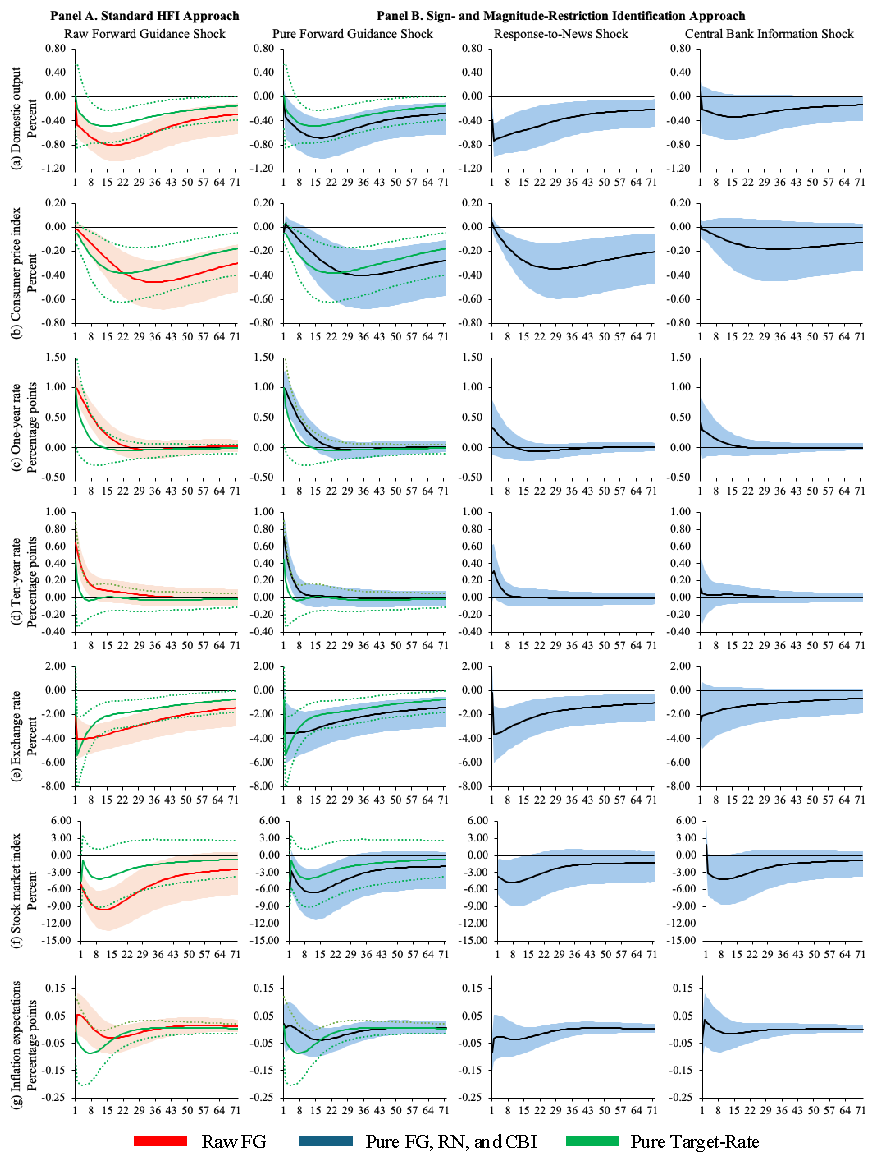
\includegraphics[width=\linewidth]{FG-cero.pdf}
}
\caption[5pt]{Impulse Responses to Forward Guidance, Response-to-News, and Central Bank Information Shocks: Exogenous High-Frequency Block Specification}
\end{center}
\begin{footnotesize} 
Notes: Responses  are  presented  for a 72-month horizon with the associated 68\% highest posterior density intervals (HPDIs).
\end{footnotesize} 
\end{figure}

\renewcommand{\thefigure}{\thesection{}.9}
\begin{figure}[htbp]
\hypertarget{Figure B.9}{}
\begin{center}
\resizebox{13cm}{!} {
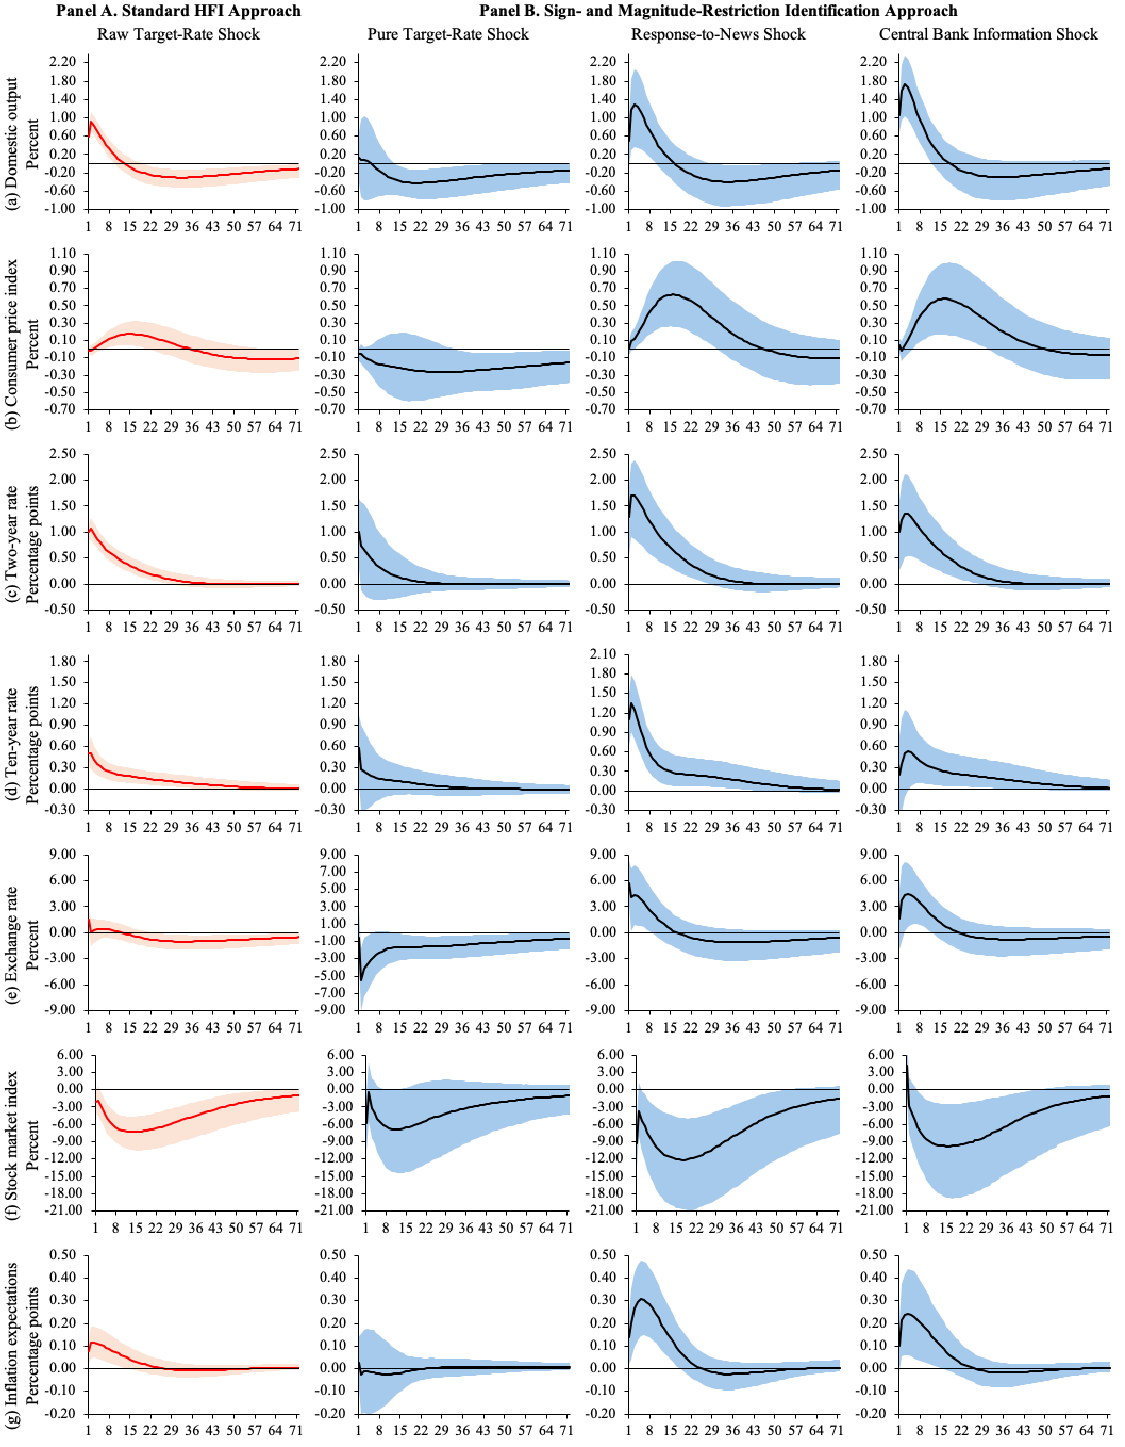
\includegraphics[width=\linewidth]{TR-2024m12_gs2.pdf}
}
\caption[5pt]{Impulse Responses to Target-Rate, Response-to-News, and Central Bank Information Shocks: Specification including the Two-Year Government Bond Yield instead of the One-Year Government Bond Yield}
\end{center}
\begin{footnotesize} 
Notes: Responses  are  presented  for a 72-month horizon with the associated 68\% highest posterior density intervals (HPDIs).
\end{footnotesize} 
\end{figure}

\renewcommand{\thefigure}{\thesection{}.10}
\begin{figure}[htbp]
\hypertarget{Figure B.10}{}
\begin{center}
\resizebox{14cm}{!} {
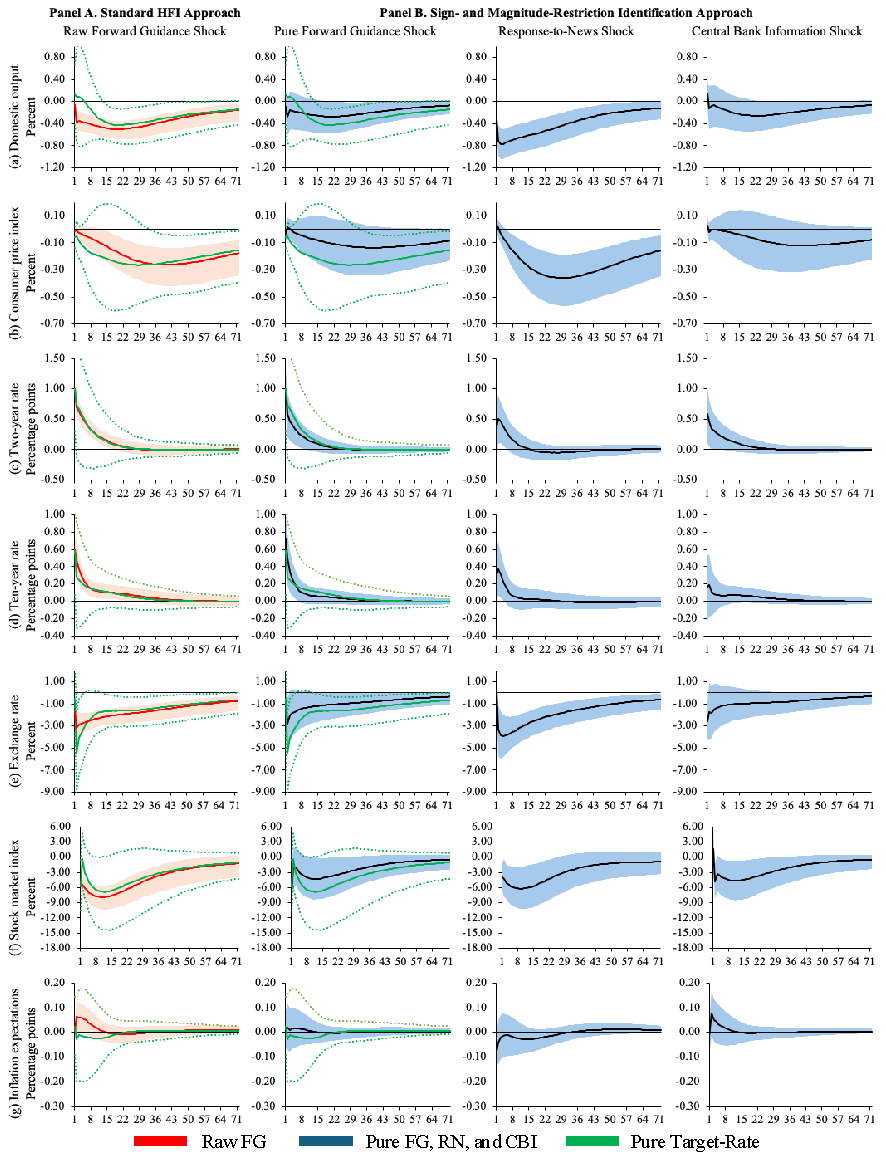
\includegraphics[width=\linewidth]{FG-2024m12_gs2.pdf}
}
\caption[5pt]{Impulse Responses to Forward Guidance, Response-to-News, and Central Bank Information Shocks: Specification including the Two-Year Government Bond Yield instead of the One-Year Government Bond Yield}
\end{center}
\begin{footnotesize} 
Notes: Responses  are  presented  for a 72-month horizon with the associated 68\% highest posterior density intervals (HPDIs).
\end{footnotesize} 
\end{figure}

\renewcommand{\thefigure}{\thesection{}.11}
\begin{figure}[htbp]
\hypertarget{Figure B.11}{}
\begin{center}
\resizebox{12cm}{!} {
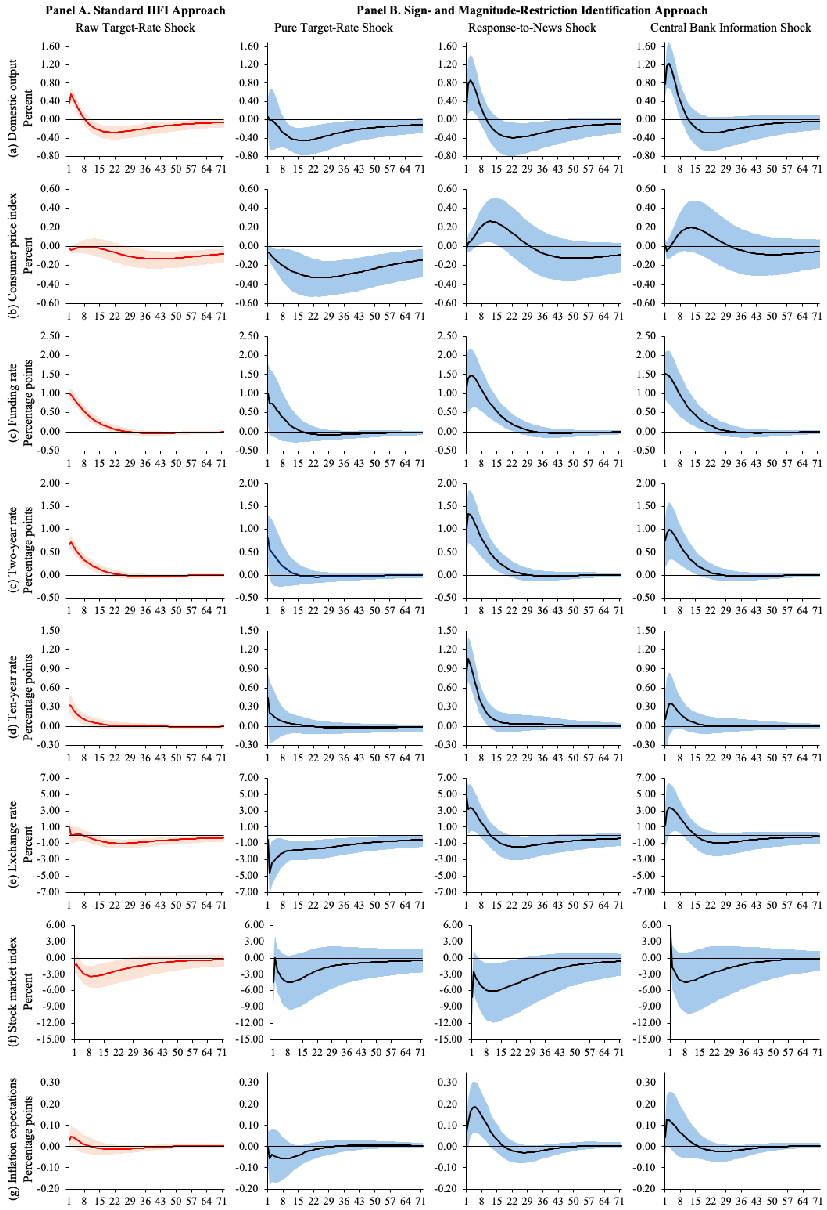
\includegraphics[width=\linewidth]{TR-2024m12_Fund_and_gs2.pdf}
}
\caption[5pt]{Impulse Responses to Target-Rate, Response-to-News, and Central Bank Information Shocks: Specification including the Interbank Funding Interest Rate and the Two-Year Government Bond Yield}
\end{center}
\begin{footnotesize} 
Notes: Responses  are  presented  for a 72-month horizon with the associated 68\% highest posterior density intervals (HPDIs).
\end{footnotesize} 
\end{figure}

\renewcommand{\thefigure}{\thesection{}.12}
\begin{figure}[htbp]
\hypertarget{Figure B.12}{}
\begin{center}
\resizebox{12cm}{!} {
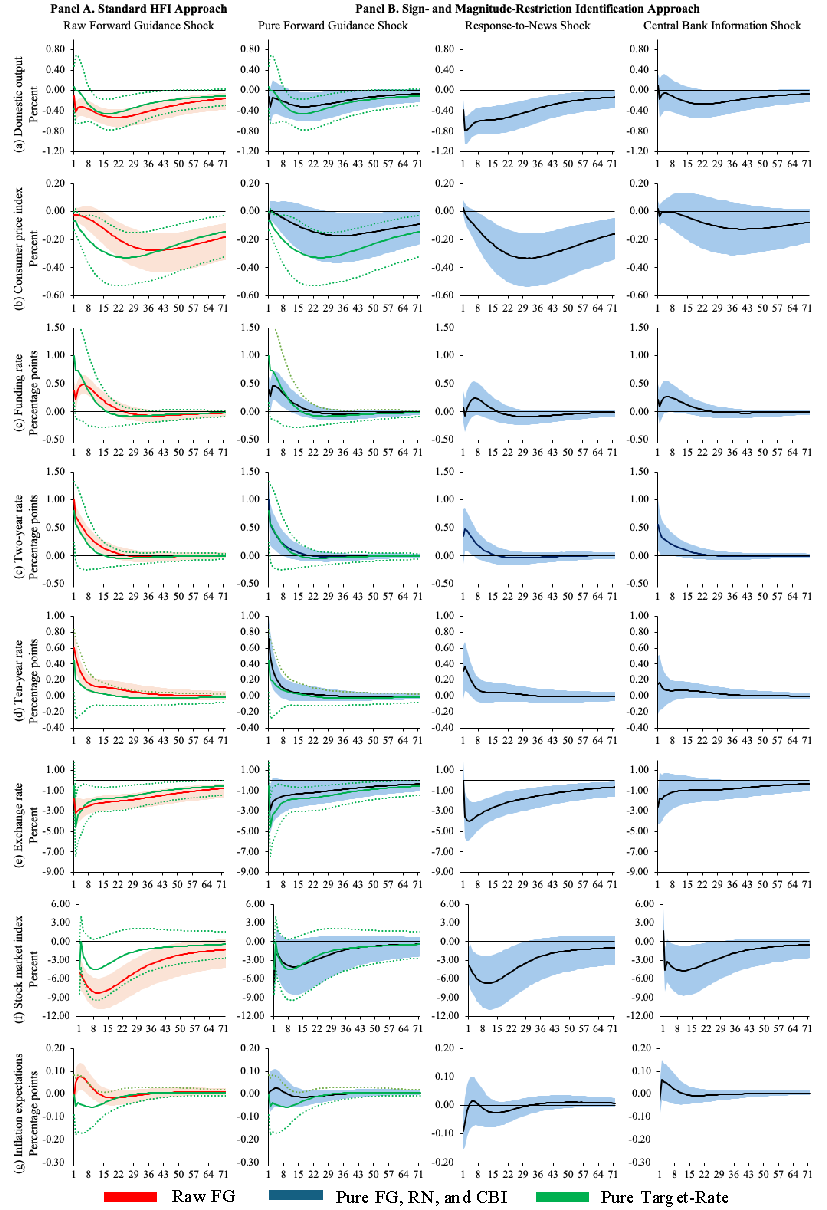
\includegraphics[width=\linewidth]{FG-2024m12_Fund_and_gs2.pdf}
}
\caption[5pt]{Impulse Responses to Forward Guidance, Response-to-News, and Central Bank Information Shocks: Specification including the Interbank Funding Interest Rate and the Two-Year Government Bond Yield}
\end{center}
\begin{footnotesize} 
Notes: Responses  are  presented  for a 72-month horizon with the associated 68\% highest posterior density intervals (HPDIs).
\end{footnotesize} 
\end{figure}

\renewcommand{\thefigure}{\thesection{}.13}
\begin{figure}[htbp]
\hypertarget{Figure B.13}{}
\begin{center}
\resizebox{14cm}{!} {
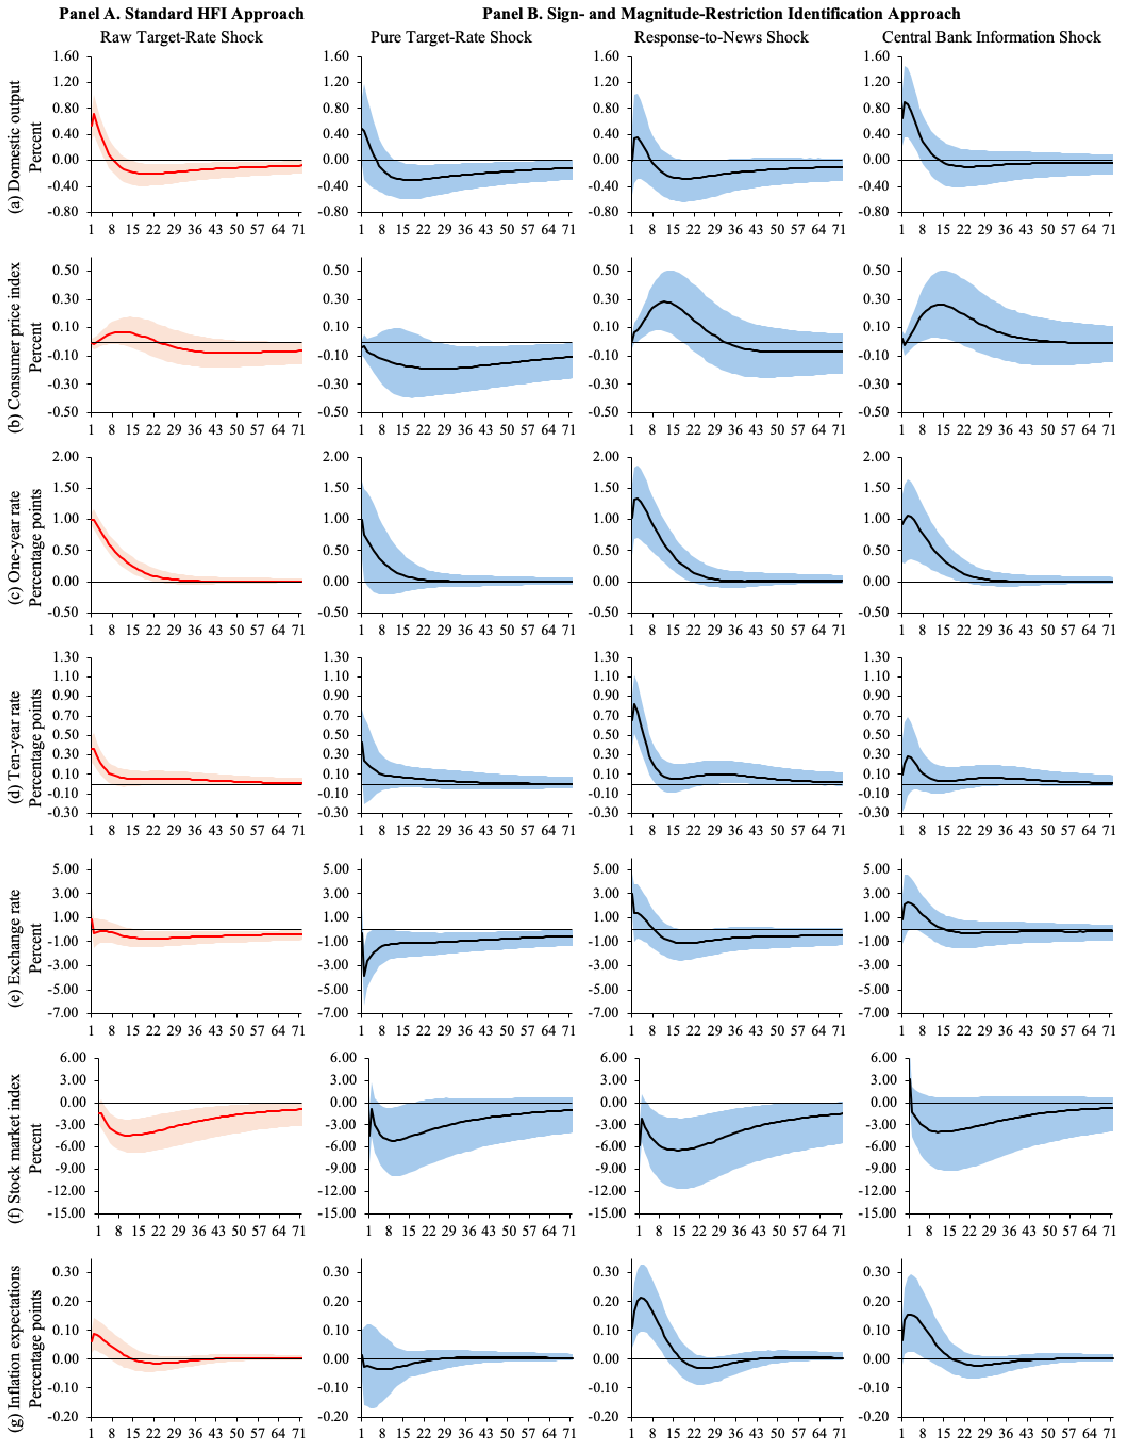
\includegraphics[width=\linewidth]{TR_igae.pdf}
}
\caption[5pt]{Impulse Responses to Target-Rate, Response-to-News, and Central Bank Information Shocks: Specification including IGAE instead of Interpolated GDP}
\end{center}
\begin{footnotesize} 
Notes: Responses  are  presented  for a 72-month horizon with the associated 68\% highest posterior density intervals (HPDIs).
\end{footnotesize} 
\end{figure}

\renewcommand{\thefigure}{\thesection{}.14}
\begin{figure}[htbp]
\hypertarget{Figure B.14}{}
\begin{center}
\resizebox{14cm}{!} {
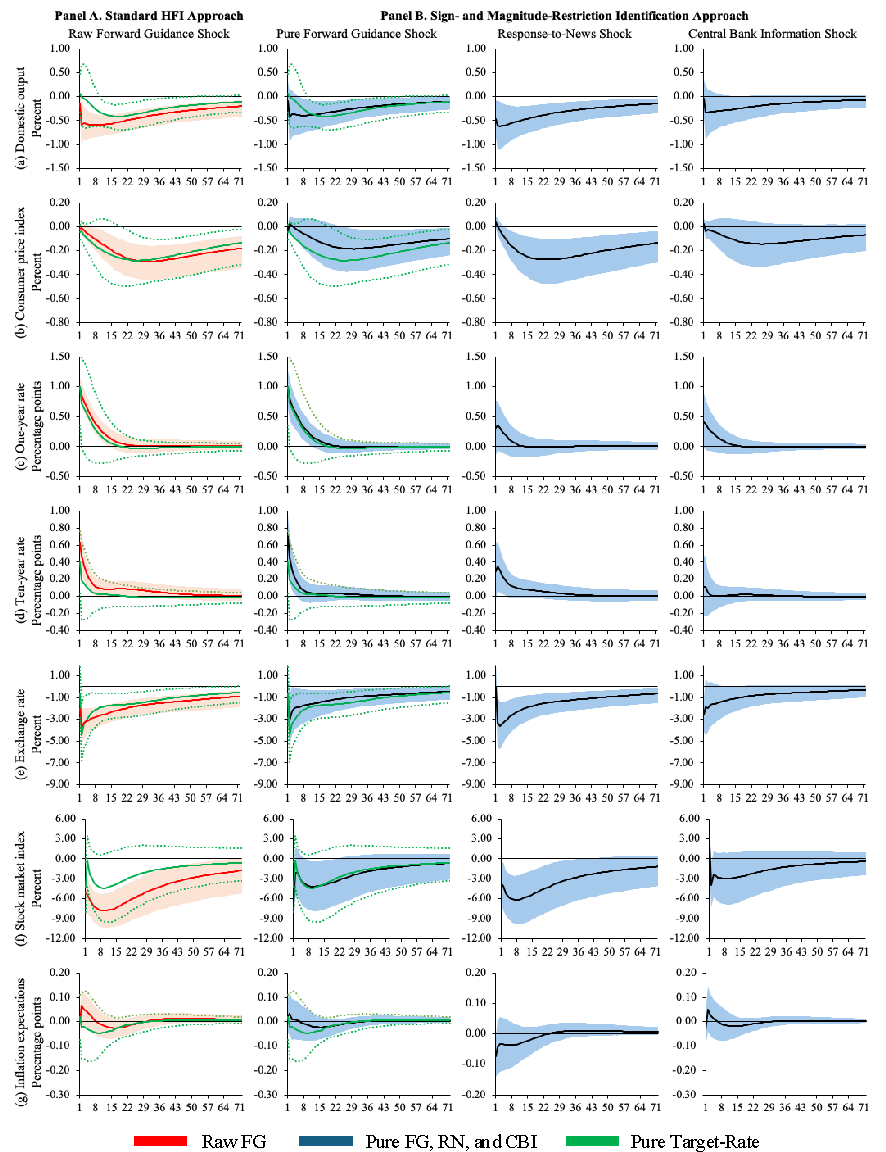
\includegraphics[width=\linewidth]{FG-igae.pdf}
}
\caption[5pt]{Impulse Responses to Forward Guidance, Response-to-News, and Central Bank Information Shocks: Specification including IGAE instead of Interpolated GDP}
\end{center}
\begin{footnotesize} 
Notes: Responses  are  presented  for a 72-month horizon with the associated 68\% highest posterior density intervals (HPDIs).
\end{footnotesize} 
\end{figure}


\renewcommand{\thefigure}{\thesection{}.15}
\begin{figure}[htbp]
\hypertarget{Figure B.15}{}
\begin{center}
\resizebox{14cm}{!} {
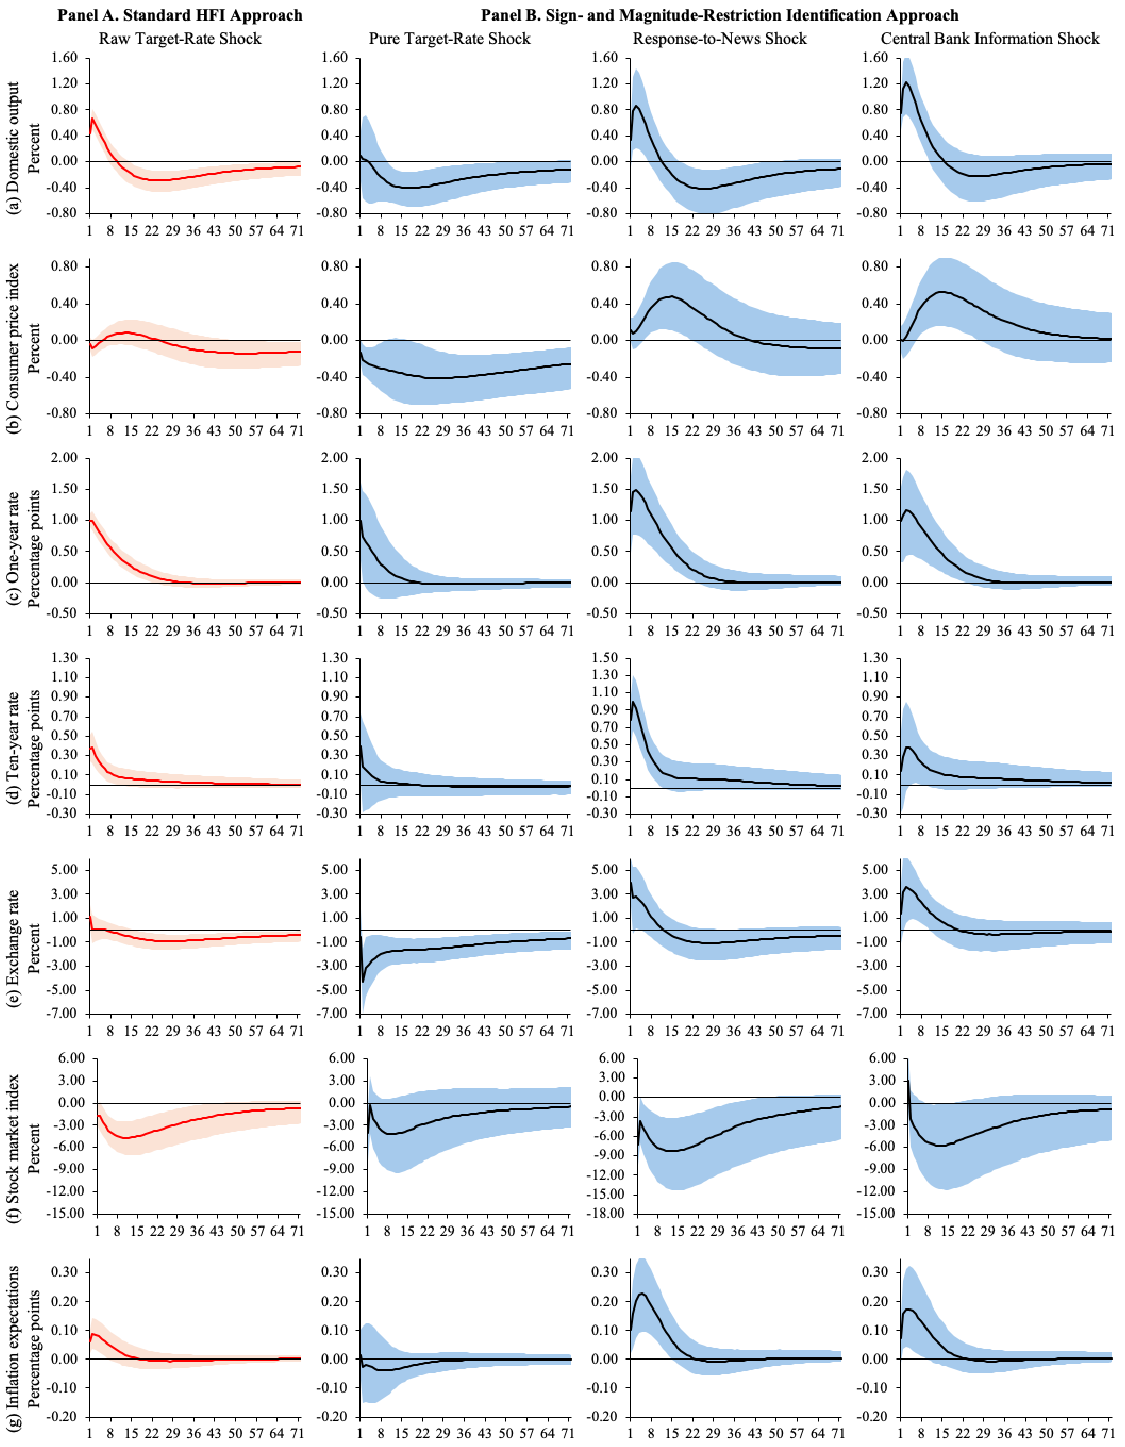
\includegraphics[width=\linewidth]{TR_inpc.pdf}
}
\caption[5pt]{Impulse Responses to Target-Rate, Response-to-News, and Central Bank Information Shocks: Specification including Headline INPC instead of Core INPC}
\end{center}
\begin{footnotesize} 
Notes: Responses  are  presented  for a 72-month horizon with the associated 68\% highest posterior density intervals (HPDIs).
\end{footnotesize} 
\end{figure}

\renewcommand{\thefigure}{\thesection{}.16}
\begin{figure}[htbp]
\hypertarget{Figure B.16}{}
\begin{center}
\resizebox{14cm}{!} {
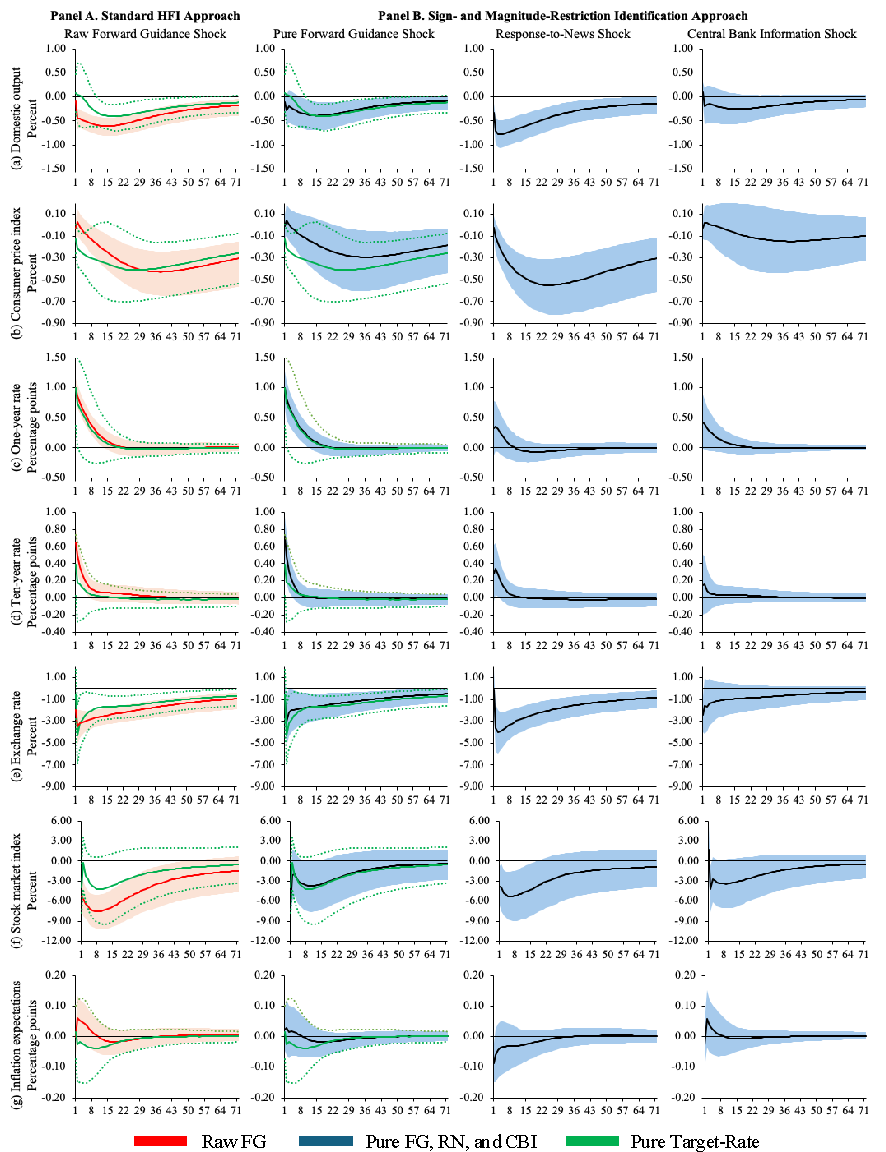
\includegraphics[width=\linewidth]{FG-inpc.pdf}
}
\caption[5pt]{Impulse Responses to Forward Guidance, Response-to-News, and Central Bank Information Shocks: Specification including Headline INPC instead of Core INPC}
\end{center}
\begin{footnotesize} 
Notes: Responses  are  presented  for a 72-month horizon with the associated 68\% highest posterior density intervals (HPDIs).
\end{footnotesize} 
\end{figure}

\renewcommand{\thefigure}{\thesection{}.17}
\begin{figure}[htbp]
\hypertarget{Figure B.17}{}
\begin{center}
\resizebox{14cm}{!} {
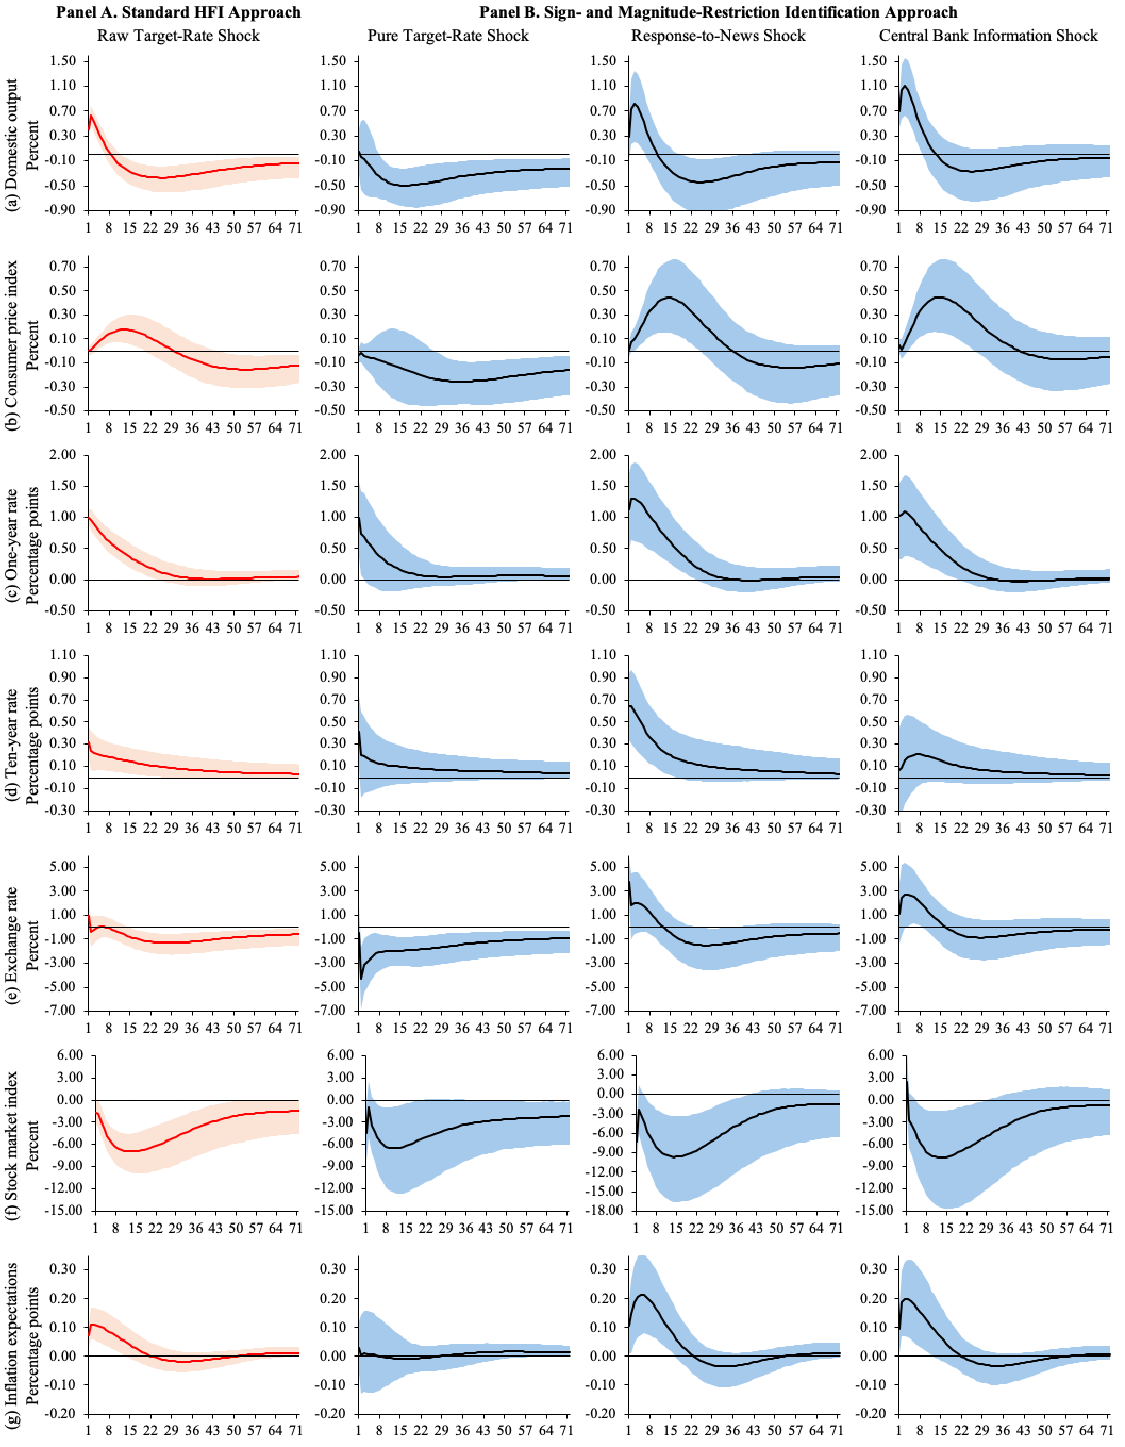
\includegraphics[width=\linewidth]{TR-2024m12_shadow.pdf}
}
\caption[5pt]{Impulse Responses to Target-Rate, Response-to-News, and Central Bank Information Shocks: Specification including the Shadow Rate instead of the U.S. 2-Year Treasury Yield}
\end{center}
\begin{footnotesize} 
Notes: Responses  are  presented  for a 72-month horizon with the associated 68\% highest posterior density intervals (HPDIs).
\end{footnotesize} 
\end{figure}

\renewcommand{\thefigure}{\thesection{}.18}
\begin{figure}[htbp]
\hypertarget{Figure B.18}{}
\begin{center}
\resizebox{14cm}{!} {
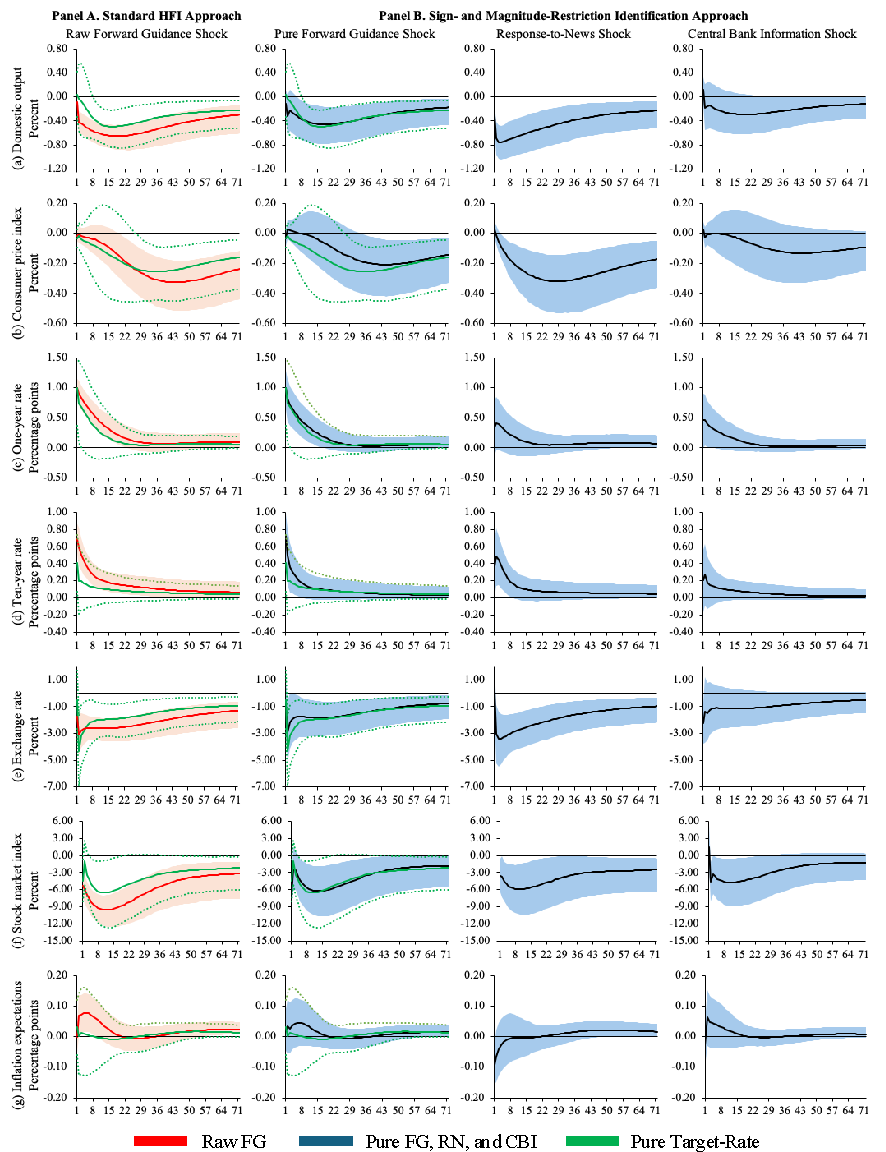
\includegraphics[width=\linewidth]{FG-2024m12_shadow.pdf}
}
\caption[5pt]{Impulse Responses to Forward Guidance, Response-to-News, and Central Bank Information Shocks: Specification including the Shadow Rate instead of the U.S. 2-Year Treasury Yield}
\end{center}
\begin{footnotesize} 
Notes: Responses  are  presented  for a 72-month horizon with the associated 68\% highest posterior density intervals (HPDIs).
\end{footnotesize} 
\end{figure}


\renewcommand{\thefigure}{\thesection{}.19}
\begin{figure}[htbp]
\hypertarget{Figure B.19}{}
\begin{center}
\resizebox{14cm}{!} {
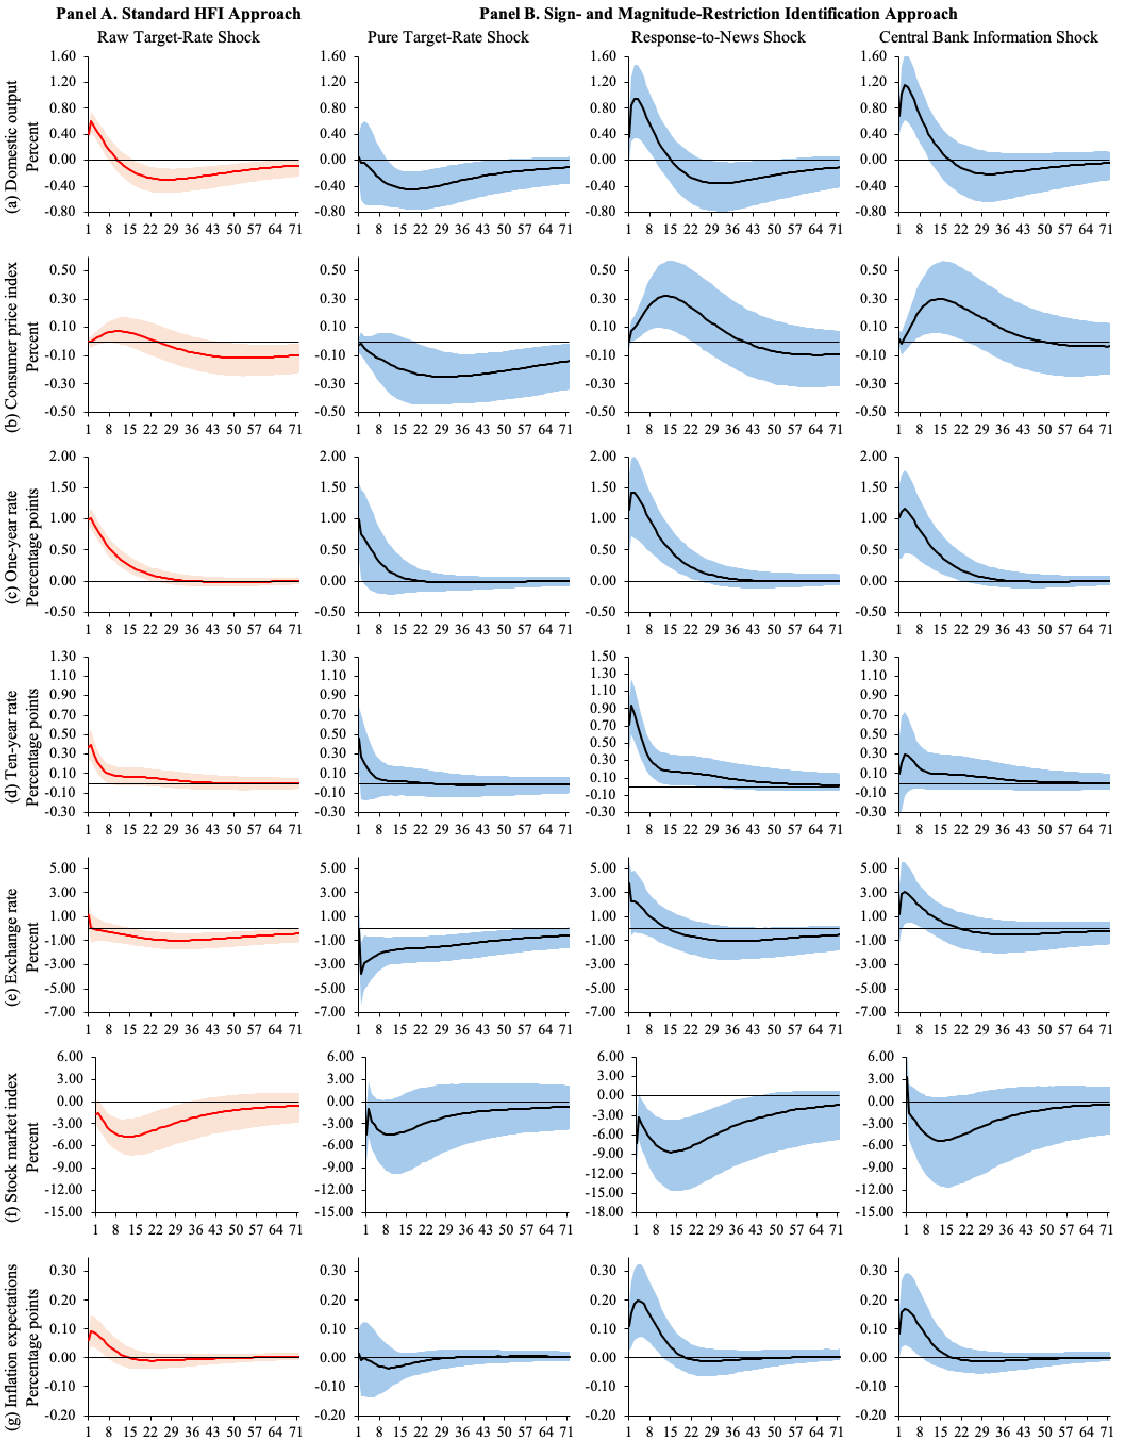
\includegraphics[width=\linewidth]{TR-extradumm_2012.pdf}
}
\caption[5pt]{Impulse Responses to Target-Rate, Response-to-News, and Central Bank Information Shocks: Pandemic Dummies Extended Through December 2020}
\end{center}
\begin{footnotesize} 
Notes: Responses  are  presented  for a 72-month horizon with the associated 68\% highest posterior density intervals (HPDIs).
\end{footnotesize} 
\end{figure}

\renewcommand{\thefigure}{\thesection{}.20}
\begin{figure}[htbp]
\hypertarget{Figure B.20}{}
\begin{center}
\resizebox{14cm}{!} {
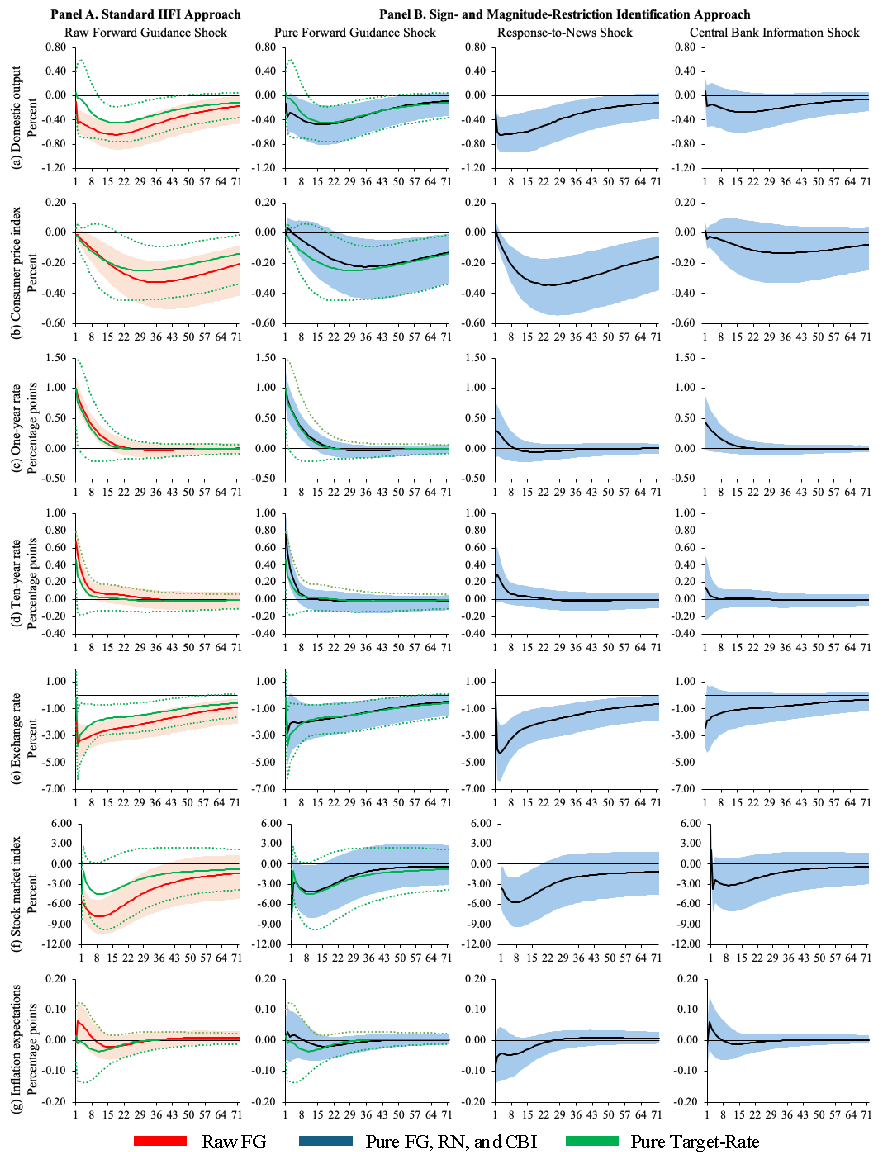
\includegraphics[width=\linewidth]{FG-extradum2012.pdf}
}
\caption[5pt]{Impulse Responses to Forward Guidance, Response-to-News, and Central Bank Information Shocks: Pandemic Dummies Extended Through December 2020}
\end{center}
\begin{footnotesize} 
Notes: Responses  are  presented  for a 72-month horizon with the associated 68\% highest posterior density intervals (HPDIs).
\end{footnotesize} 
\end{figure}

\renewcommand{\thefigure}{\thesection{}.21}
\begin{figure}[htbp]
\hypertarget{Figure B.21}{}
\begin{center}
\resizebox{14cm}{!} {
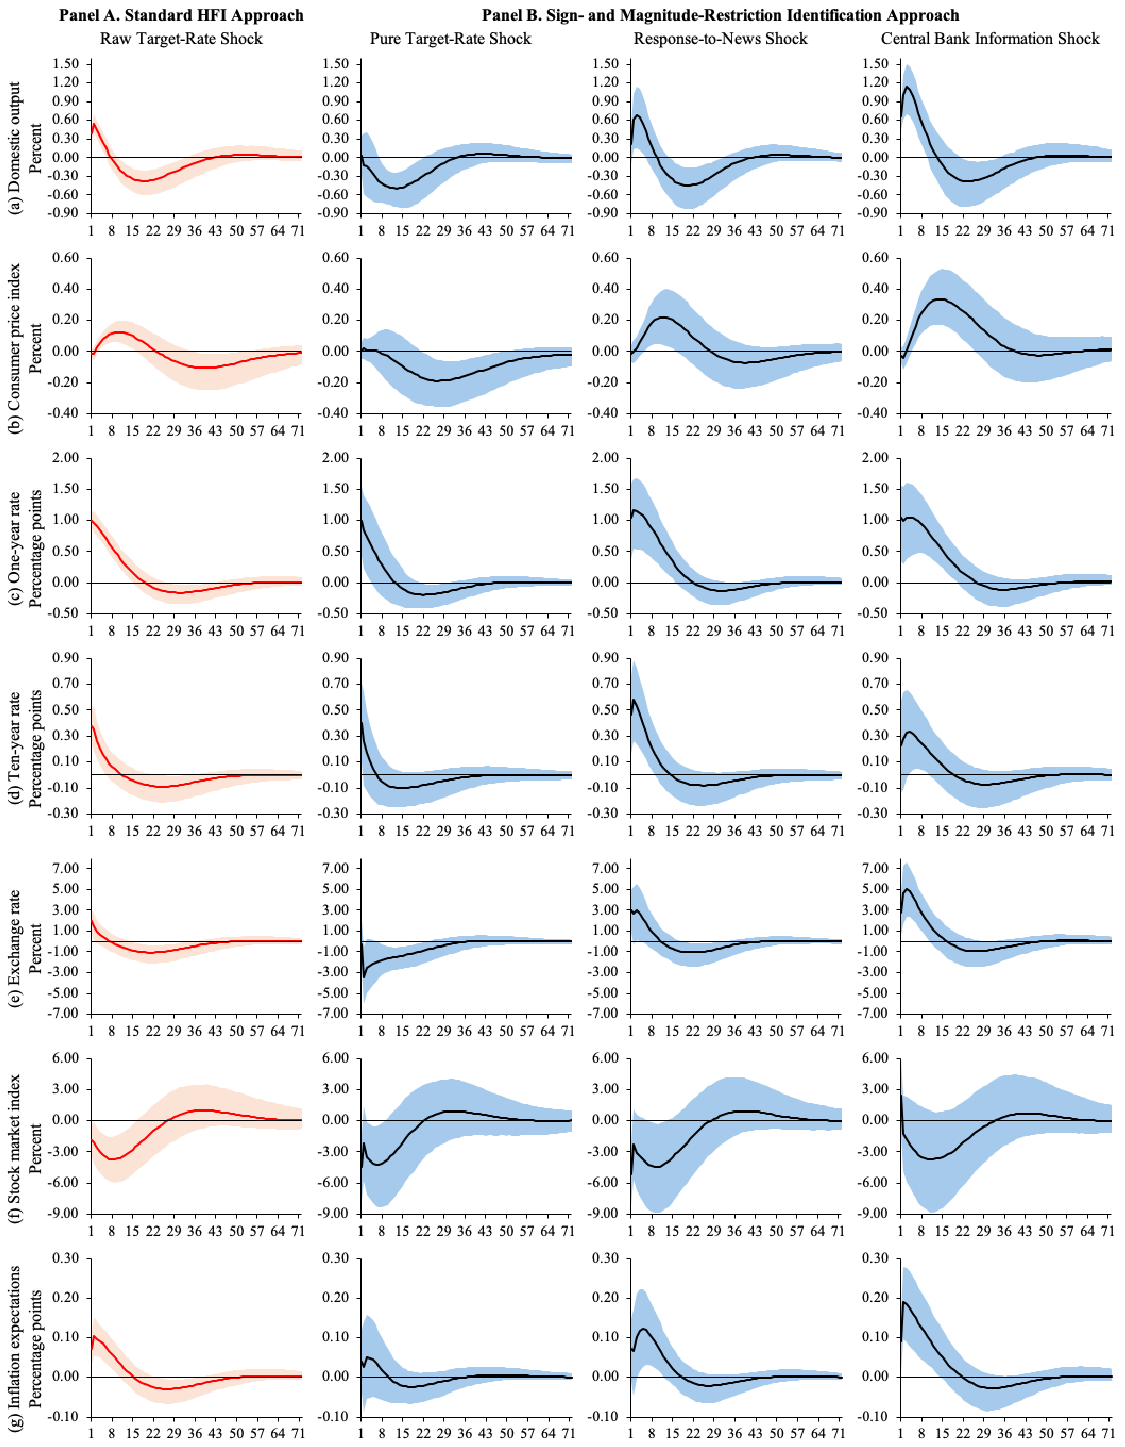
\includegraphics[width=\linewidth]{TR-2019.pdf}
}
\caption[5pt]{Impulse Responses to Target-Rate, Response-to-News, and Central Bank Information Shocks: Sample 2002-2019}
\end{center}
\begin{footnotesize} 
Notes: Responses  are  presented  for a 72-month horizon with the associated 68\% highest posterior density intervals (HPDIs).
\end{footnotesize} 
\end{figure}

\renewcommand{\thefigure}{\thesection{}.22}
\begin{figure}[htbp]
\hypertarget{Figure B.22}{}
\begin{center}
\resizebox{14cm}{!} {
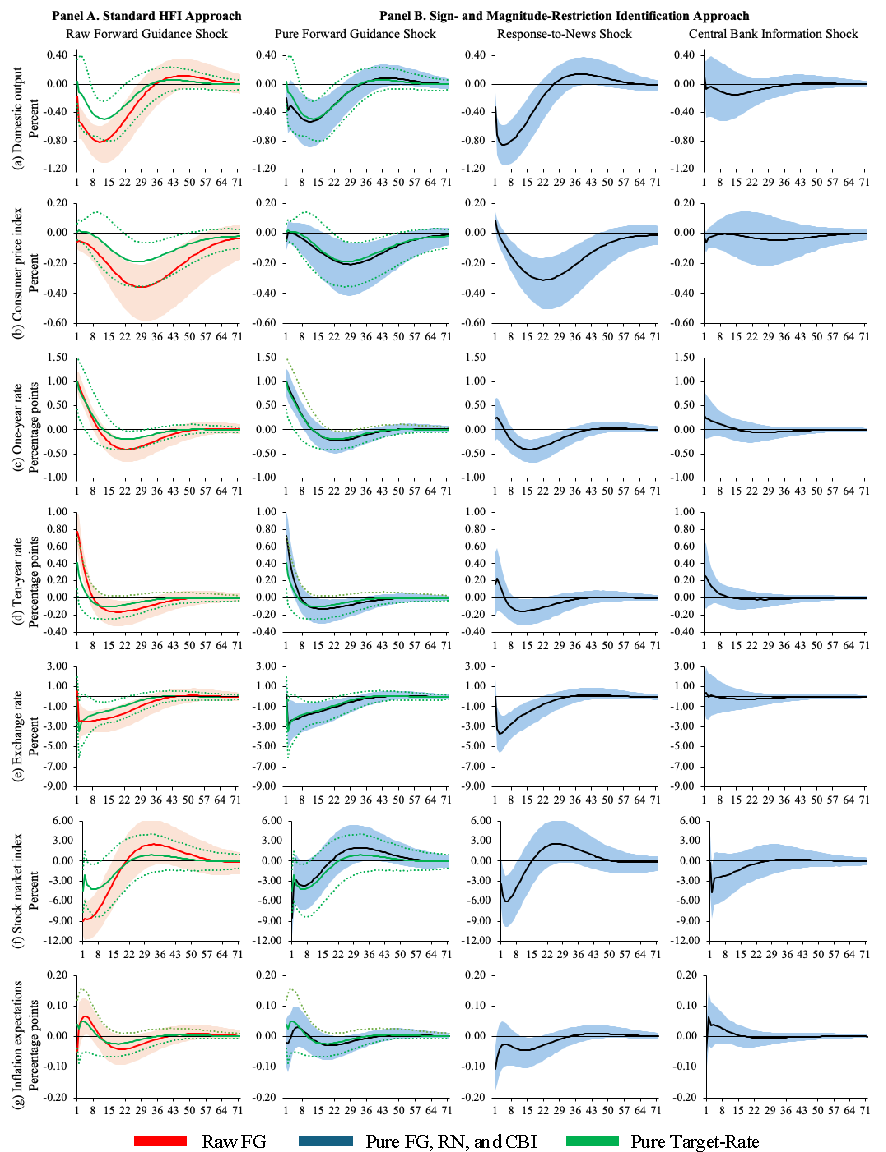
\includegraphics[width=\linewidth]{FG-2019m12.pdf}
}
\caption[5pt]{Impulse Responses to Forward Guidance, Response-to-News, and Central Bank Information Shocks: Sample 2002-2019}
\end{center}
\begin{footnotesize} 
Notes: Responses  are  presented  for a 72-month horizon with the associated 68\% highest posterior density intervals (HPDIs).
\end{footnotesize} 
\end{figure}





\renewcommand{\thefigure}{\thesection{}.23}
\begin{figure}[htbp]
\hypertarget{Figure B.23}{}
\begin{center}
\resizebox{14cm}{!} {
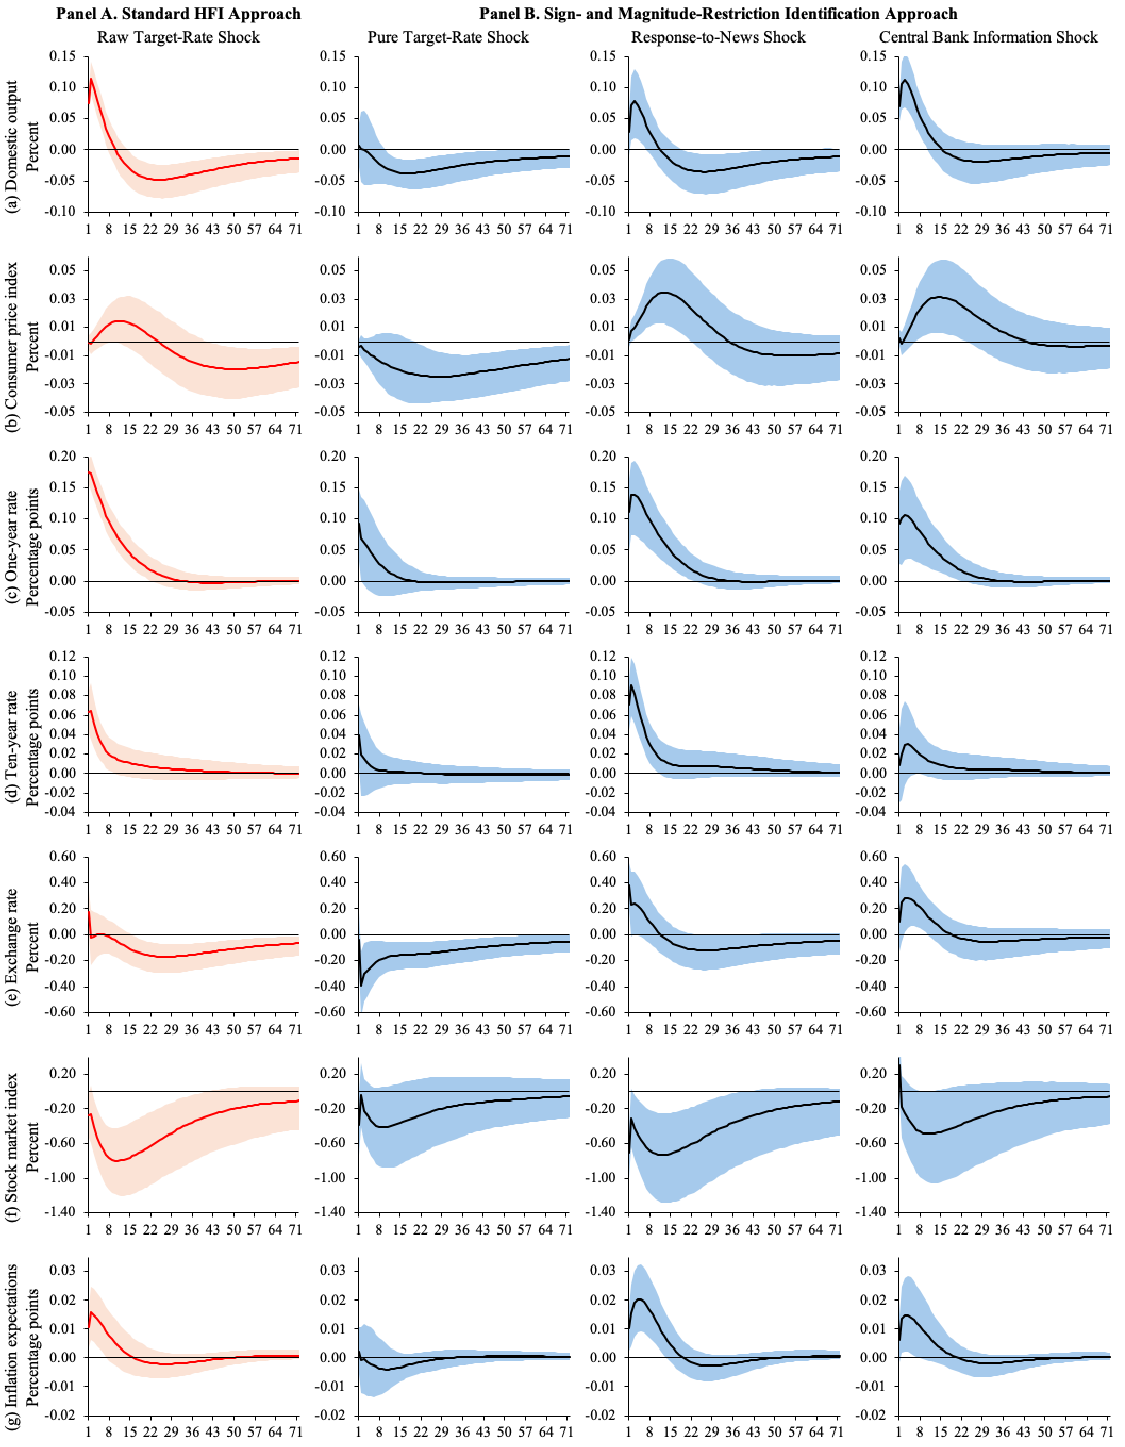
\includegraphics[width=\linewidth]{TR-1sd.pdf}
}
\caption[5pt]{Impulse Responses to Target-Rate, Response-to-News, and Central Bank Information Shocks without Standardization}
\end{center}
\begin{footnotesize} 
Notes: Responses  are  presented  for a 72-month horizon with the associated 68\% highest posterior density intervals (HPDIs).
\end{footnotesize} 
\end{figure}

\renewcommand{\thefigure}{\thesection{}.24}
\begin{figure}[htbp]
\hypertarget{Figure B.24}{}
\begin{center}
\resizebox{14cm}{!} {
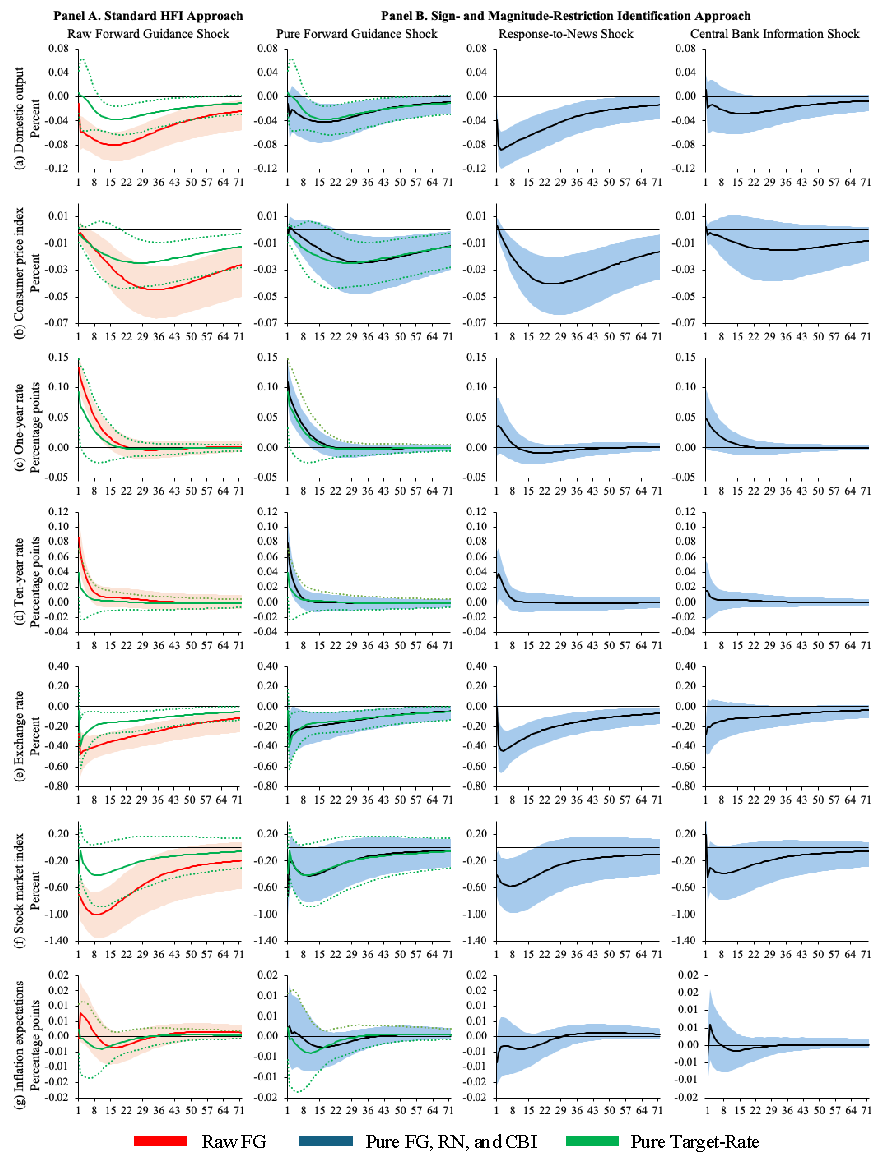
\includegraphics[width=\linewidth]{FG-1sd.pdf}
}
\caption[5pt]{Impulse Responses to Forward Guidance, Response-to-News, and Central Bank Information Shocks without Standardization}
\end{center}
\begin{footnotesize} 
Notes: Responses  are  presented  for a 72-month horizon with the associated 68\% highest posterior density intervals (HPDIs).
\end{footnotesize} 
\end{figure}


\end{document}


